% -------------------------------------------------------------------------------
\chapter{Addressing Missing Sources with Adversarial Support-Matching}\label{ch:supmatch}
% -------------------------------------------------------------------------------
% \documentclass{article} % For LaTeX2e
% \usepackage{tmlr,times}

% Optional math commands from https://github.com/goodfeli/dlbook_notation.
% %%%%% NEW MATH DEFINITIONS %%%%%

\usepackage{amsmath,amsfonts,bm}

% Mark sections of captions for referring to divisions of figures
\newcommand{\figleft}{{\em (Left)}}
\newcommand{\figcenter}{{\em (Center)}}
\newcommand{\figright}{{\em (Right)}}
\newcommand{\figtop}{{\em (Top)}}
\newcommand{\figbottom}{{\em (Bottom)}}
\newcommand{\captiona}{{\em (a)}}
\newcommand{\captionb}{{\em (b)}}
\newcommand{\captionc}{{\em (c)}}
\newcommand{\captiond}{{\em (d)}}

% Highlight a newly defined term
\newcommand{\newterm}[1]{{\bf #1}}


% Figure reference, lower-case.
\def\figref#1{figure~\ref{#1}}
% Figure reference, capital. For start of sentence
\def\Figref#1{Figure~\ref{#1}}
\def\twofigref#1#2{figures \ref{#1} and \ref{#2}}
\def\quadfigref#1#2#3#4{figures \ref{#1}, \ref{#2}, \ref{#3} and \ref{#4}}
% Section reference, lower-case.
\def\secref#1{section~\ref{#1}}
% Section reference, capital.
\def\Secref#1{Section~\ref{#1}}
% Reference to two sections.
\def\twosecrefs#1#2{sections \ref{#1} and \ref{#2}}
% Reference to three sections.
\def\secrefs#1#2#3{sections \ref{#1}, \ref{#2} and \ref{#3}}
% Appendix reference, lower-case.
\def\appref#1{appendix~\ref{#1}}
% Appendix reference, capital.
\def\Appref#1{Appendix~\ref{#1}}
% Reference to an equation, lower-case.
\def\eqref#1{equation~\ref{#1}}
% Reference to an equation, upper case
\def\Eqref#1{Equation~\ref{#1}}
% A raw reference to an equation---avoid using if possible
\def\plaineqref#1{\ref{#1}}
% Reference to a chapter, lower-case.
\def\chapref#1{chapter~\ref{#1}}
% Reference to a Chapter, upper case.
\def\Chapref#1{Chapter~\ref{#1}}
\def\twochaprefs#1#2{chapters \ref{#1} and \ref{#2}}
% Reference to a range of chapters
\def\rangechapref#1#2{chapters \ref{#1}--\ref{#2}}
% Reference to a range of chapters, upper case
\def\Rangechapref#1#2{Chapters \ref{#1}--\ref{#2}}
% Reference to an algorithm, lower-case.
\def\algref#1{algorithm~\ref{#1}}
% Reference to an algorithm, upper case.
\def\Algref#1{Algorithm~\ref{#1}}
\def\twoalgref#1#2{algorithms \ref{#1} and \ref{#2}}
\def\Twoalgref#1#2{Algorithms \ref{#1} and \ref{#2}}
% Reference to a part, lower case
\def\partref#1{part~\ref{#1}}
% Reference to a part, upper case
\def\Partref#1{Part~\ref{#1}}
\def\twopartref#1#2{parts \ref{#1} and \ref{#2}}

\def\ceil#1{\lceil #1 \rceil}
\def\floor#1{\lfloor #1 \rfloor}
\def\1{\bm{1}}
\newcommand{\train}{\mathcal{D}}
\newcommand{\valid}{\mathcal{D_{\mathrm{valid}}}}
\newcommand{\test}{\mathcal{D_{\mathrm{test}}}}

\def\eps{{\epsilon}}


% Random variables
\def\reta{{\textnormal{$\eta$}}}
\def\ra{{\textnormal{a}}}
\def\rb{{\textnormal{b}}}
\def\rc{{\textnormal{c}}}
\def\rd{{\textnormal{d}}}
\def\re{{\textnormal{e}}}
\def\rf{{\textnormal{f}}}
\def\rg{{\textnormal{g}}}
\def\rh{{\textnormal{h}}}
\def\ri{{\textnormal{i}}}
\def\rj{{\textnormal{j}}}
\def\rk{{\textnormal{k}}}
\def\rl{{\textnormal{l}}}
% rm is already a command, just don't name any random variables m
\def\rn{{\textnormal{n}}}
\def\ro{{\textnormal{o}}}
\def\rp{{\textnormal{p}}}
\def\rq{{\textnormal{q}}}
\def\rr{{\textnormal{r}}}
\def\rs{{\textnormal{s}}}
\def\rt{{\textnormal{t}}}
\def\ru{{\textnormal{u}}}
\def\rv{{\textnormal{v}}}
\def\rw{{\textnormal{w}}}
\def\rx{{\textnormal{x}}}
\def\ry{{\textnormal{y}}}
\def\rz{{\textnormal{z}}}

% Random vectors
\def\rvepsilon{{\mathbf{\epsilon}}}
\def\rvtheta{{\mathbf{\theta}}}
\def\rva{{\mathbf{a}}}
\def\rvb{{\mathbf{b}}}
\def\rvc{{\mathbf{c}}}
\def\rvd{{\mathbf{d}}}
\def\rve{{\mathbf{e}}}
\def\rvf{{\mathbf{f}}}
\def\rvg{{\mathbf{g}}}
\def\rvh{{\mathbf{h}}}
\def\rvu{{\mathbf{i}}}
\def\rvj{{\mathbf{j}}}
\def\rvk{{\mathbf{k}}}
\def\rvl{{\mathbf{l}}}
\def\rvm{{\mathbf{m}}}
\def\rvn{{\mathbf{n}}}
\def\rvo{{\mathbf{o}}}
\def\rvp{{\mathbf{p}}}
\def\rvq{{\mathbf{q}}}
\def\rvr{{\mathbf{r}}}
\def\rvs{{\mathbf{s}}}
\def\rvt{{\mathbf{t}}}
\def\rvu{{\mathbf{u}}}
\def\rvv{{\mathbf{v}}}
\def\rvw{{\mathbf{w}}}
\def\rvx{{\mathbf{x}}}
\def\rvy{{\mathbf{y}}}
\def\rvz{{\mathbf{z}}}

% Elements of random vectors
\def\erva{{\textnormal{a}}}
\def\ervb{{\textnormal{b}}}
\def\ervc{{\textnormal{c}}}
\def\ervd{{\textnormal{d}}}
\def\erve{{\textnormal{e}}}
\def\ervf{{\textnormal{f}}}
\def\ervg{{\textnormal{g}}}
\def\ervh{{\textnormal{h}}}
\def\ervi{{\textnormal{i}}}
\def\ervj{{\textnormal{j}}}
\def\ervk{{\textnormal{k}}}
\def\ervl{{\textnormal{l}}}
\def\ervm{{\textnormal{m}}}
\def\ervn{{\textnormal{n}}}
\def\ervo{{\textnormal{o}}}
\def\ervp{{\textnormal{p}}}
\def\ervq{{\textnormal{q}}}
\def\ervr{{\textnormal{r}}}
\def\ervs{{\textnormal{s}}}
\def\ervt{{\textnormal{t}}}
\def\ervu{{\textnormal{u}}}
\def\ervv{{\textnormal{v}}}
\def\ervw{{\textnormal{w}}}
\def\ervx{{\textnormal{x}}}
\def\ervy{{\textnormal{y}}}
\def\ervz{{\textnormal{z}}}

% Random matrices
\def\rmA{{\mathbf{A}}}
\def\rmB{{\mathbf{B}}}
\def\rmC{{\mathbf{C}}}
\def\rmD{{\mathbf{D}}}
\def\rmE{{\mathbf{E}}}
\def\rmF{{\mathbf{F}}}
\def\rmG{{\mathbf{G}}}
\def\rmH{{\mathbf{H}}}
\def\rmI{{\mathbf{I}}}
\def\rmJ{{\mathbf{J}}}
\def\rmK{{\mathbf{K}}}
\def\rmL{{\mathbf{L}}}
\def\rmM{{\mathbf{M}}}
\def\rmN{{\mathbf{N}}}
\def\rmO{{\mathbf{O}}}
\def\rmP{{\mathbf{P}}}
\def\rmQ{{\mathbf{Q}}}
\def\rmR{{\mathbf{R}}}
\def\rmS{{\mathbf{S}}}
\def\rmT{{\mathbf{T}}}
\def\rmU{{\mathbf{U}}}
\def\rmV{{\mathbf{V}}}
\def\rmW{{\mathbf{W}}}
\def\rmX{{\mathbf{X}}}
\def\rmY{{\mathbf{Y}}}
\def\rmZ{{\mathbf{Z}}}

% Elements of random matrices
\def\ermA{{\textnormal{A}}}
\def\ermB{{\textnormal{B}}}
\def\ermC{{\textnormal{C}}}
\def\ermD{{\textnormal{D}}}
\def\ermE{{\textnormal{E}}}
\def\ermF{{\textnormal{F}}}
\def\ermG{{\textnormal{G}}}
\def\ermH{{\textnormal{H}}}
\def\ermI{{\textnormal{I}}}
\def\ermJ{{\textnormal{J}}}
\def\ermK{{\textnormal{K}}}
\def\ermL{{\textnormal{L}}}
\def\ermM{{\textnormal{M}}}
\def\ermN{{\textnormal{N}}}
\def\ermO{{\textnormal{O}}}
\def\ermP{{\textnormal{P}}}
\def\ermQ{{\textnormal{Q}}}
\def\ermR{{\textnormal{R}}}
\def\ermS{{\textnormal{S}}}
\def\ermT{{\textnormal{T}}}
\def\ermU{{\textnormal{U}}}
\def\ermV{{\textnormal{V}}}
\def\ermW{{\textnormal{W}}}
\def\ermX{{\textnormal{X}}}
\def\ermY{{\textnormal{Y}}}
\def\ermZ{{\textnormal{Z}}}

% Vectors
\def\vzero{{\bm{0}}}
\def\vone{{\bm{1}}}
\def\vmu{{\bm{\mu}}}
\def\vtheta{{\bm{\theta}}}
\def\va{{\bm{a}}}
\def\vb{{\bm{b}}}
\def\vc{{\bm{c}}}
\def\vd{{\bm{d}}}
\def\ve{{\bm{e}}}
\def\vf{{\bm{f}}}
\def\vg{{\bm{g}}}
\def\vh{{\bm{h}}}
\def\vi{{\bm{i}}}
\def\vj{{\bm{j}}}
\def\vk{{\bm{k}}}
\def\vl{{\bm{l}}}
\def\vm{{\bm{m}}}
\def\vn{{\bm{n}}}
\def\vo{{\bm{o}}}
\def\vp{{\bm{p}}}
\def\vq{{\bm{q}}}
\def\vr{{\bm{r}}}
\def\vs{{\bm{s}}}
\def\vt{{\bm{t}}}
\def\vu{{\bm{u}}}
\def\vv{{\bm{v}}}
\def\vw{{\bm{w}}}
\def\vx{{\bm{x}}}
\def\vy{{\bm{y}}}
\def\vz{{\bm{z}}}

% Elements of vectors
\def\evalpha{{\alpha}}
\def\evbeta{{\beta}}
\def\evepsilon{{\epsilon}}
\def\evlambda{{\lambda}}
\def\evomega{{\omega}}
\def\evmu{{\mu}}
\def\evpsi{{\psi}}
\def\evsigma{{\sigma}}
\def\evtheta{{\theta}}
\def\eva{{a}}
\def\evb{{b}}
\def\evc{{c}}
\def\evd{{d}}
\def\eve{{e}}
\def\evf{{f}}
\def\evg{{g}}
\def\evh{{h}}
\def\evi{{i}}
\def\evj{{j}}
\def\evk{{k}}
\def\evl{{l}}
\def\evm{{m}}
\def\evn{{n}}
\def\evo{{o}}
\def\evp{{p}}
\def\evq{{q}}
\def\evr{{r}}
\def\evs{{s}}
\def\evt{{t}}
\def\evu{{u}}
\def\evv{{v}}
\def\evw{{w}}
\def\evx{{x}}
\def\evy{{y}}
\def\evz{{z}}

% Matrix
\def\mA{{\bm{A}}}
\def\mB{{\bm{B}}}
\def\mC{{\bm{C}}}
\def\mD{{\bm{D}}}
\def\mE{{\bm{E}}}
\def\mF{{\bm{F}}}
\def\mG{{\bm{G}}}
\def\mH{{\bm{H}}}
\def\mI{{\bm{I}}}
\def\mJ{{\bm{J}}}
\def\mK{{\bm{K}}}
\def\mL{{\bm{L}}}
\def\mM{{\bm{M}}}
\def\mN{{\bm{N}}}
\def\mO{{\bm{O}}}
\def\mP{{\bm{P}}}
\def\mQ{{\bm{Q}}}
\def\mR{{\bm{R}}}
\def\mS{{\bm{S}}}
\def\mT{{\bm{T}}}
\def\mU{{\bm{U}}}
\def\mV{{\bm{V}}}
\def\mW{{\bm{W}}}
\def\mX{{\bm{X}}}
\def\mY{{\bm{Y}}}
\def\mZ{{\bm{Z}}}
\def\mBeta{{\bm{\beta}}}
\def\mPhi{{\bm{\Phi}}}
\def\mLambda{{\bm{\Lambda}}}
\def\mSigma{{\bm{\Sigma}}}

% % Tensor
% \DeclareMathAlphabet{\mathsfit}{\encodingdefault}{\sfdefault}{m}{sl}
% \SetMathAlphabet{\mathsfit}{bold}{\encodingdefault}{\sfdefault}{bx}{n}
% \newcommand{\tens}[1]{\bm{\mathsfit{#1}}}
% \def\tA{{\tens{A}}}
% \def\tB{{\tens{B}}}
% \def\tC{{\tens{C}}}
% \def\tD{{\tens{D}}}
% \def\tE{{\tens{E}}}
% \def\tF{{\tens{F}}}
% \def\tG{{\tens{G}}}
% \def\tH{{\tens{H}}}
% \def\tI{{\tens{I}}}
% \def\tJ{{\tens{J}}}
% \def\tK{{\tens{K}}}
% \def\tL{{\tens{L}}}
% \def\tM{{\tens{M}}}
% \def\tN{{\tens{N}}}
% \def\tO{{\tens{O}}}
% \def\tP{{\tens{P}}}
% \def\tQ{{\tens{Q}}}
% \def\tR{{\tens{R}}}
% \def\tS{{\tens{S}}}
% \def\tT{{\tens{T}}}
% \def\tU{{\tens{U}}}
% \def\tV{{\tens{V}}}
% \def\tW{{\tens{W}}}
% \def\tX{{\tens{X}}}
% \def\tY{{\tens{Y}}}
% \def\tZ{{\tens{Z}}}


% Graph
\def\gA{{\mathcal{A}}}
\def\gB{{\mathcal{B}}}
\def\gC{{\mathcal{C}}}
\def\gD{{\mathcal{D}}}
\def\gE{{\mathcal{E}}}
\def\gF{{\mathcal{F}}}
\def\gG{{\mathcal{G}}}
\def\gH{{\mathcal{H}}}
\def\gI{{\mathcal{I}}}
\def\gJ{{\mathcal{J}}}
\def\gK{{\mathcal{K}}}
\def\gL{{\mathcal{L}}}
\def\gM{{\mathcal{M}}}
\def\gN{{\mathcal{N}}}
\def\gO{{\mathcal{O}}}
\def\gP{{\mathcal{P}}}
\def\gQ{{\mathcal{Q}}}
\def\gR{{\mathcal{R}}}
\def\gS{{\mathcal{S}}}
\def\gT{{\mathcal{T}}}
\def\gU{{\mathcal{U}}}
\def\gV{{\mathcal{V}}}
\def\gW{{\mathcal{W}}}
\def\gX{{\mathcal{X}}}
\def\gY{{\mathcal{Y}}}
\def\gZ{{\mathcal{Z}}}

% Sets
\def\sA{{\mathbb{A}}}
\def\sB{{\mathbb{B}}}
\def\sC{{\mathbb{C}}}
\def\sD{{\mathbb{D}}}
% Don't use a set called E, because this would be the same as our symbol
% for expectation.
\def\sF{{\mathbb{F}}}
\def\sG{{\mathbb{G}}}
\def\sH{{\mathbb{H}}}
\def\sI{{\mathbb{I}}}
\def\sJ{{\mathbb{J}}}
\def\sK{{\mathbb{K}}}
\def\sL{{\mathbb{L}}}
\def\sM{{\mathbb{M}}}
\def\sN{{\mathbb{N}}}
\def\sO{{\mathbb{O}}}
\def\sP{{\mathbb{P}}}
\def\sQ{{\mathbb{Q}}}
\def\sR{{\mathbb{R}}}
\def\sS{{\mathbb{S}}}
\def\sT{{\mathbb{T}}}
\def\sU{{\mathbb{U}}}
\def\sV{{\mathbb{V}}}
\def\sW{{\mathbb{W}}}
\def\sX{{\mathbb{X}}}
\def\sY{{\mathbb{Y}}}
\def\sZ{{\mathbb{Z}}}

% Entries of a matrix
\def\emLambda{{\Lambda}}
\def\emA{{A}}
\def\emB{{B}}
\def\emC{{C}}
\def\emD{{D}}
\def\emE{{E}}
\def\emF{{F}}
\def\emG{{G}}
\def\emH{{H}}
\def\emI{{I}}
\def\emJ{{J}}
\def\emK{{K}}
\def\emL{{L}}
\def\emM{{M}}
\def\emN{{N}}
\def\emO{{O}}
\def\emP{{P}}
\def\emQ{{Q}}
\def\emR{{R}}
\def\emS{{S}}
\def\emT{{T}}
\def\emU{{U}}
\def\emV{{V}}
\def\emW{{W}}
\def\emX{{X}}
\def\emY{{Y}}
\def\emZ{{Z}}
\def\emSigma{{\Sigma}}

% entries of a tensor
% Same font as tensor, without \bm wrapper
% \newcommand{\etens}[1]{\mathsfit{#1}}
% \def\etLambda{{\etens{\Lambda}}}
% \def\etA{{\etens{A}}}
% \def\etB{{\etens{B}}}
% \def\etC{{\etens{C}}}
% \def\etD{{\etens{D}}}
% \def\etE{{\etens{E}}}
% \def\etF{{\etens{F}}}
% \def\etG{{\etens{G}}}
% \def\etH{{\etens{H}}}
% \def\etI{{\etens{I}}}
% \def\etJ{{\etens{J}}}
% \def\etK{{\etens{K}}}
% \def\etL{{\etens{L}}}
% \def\etM{{\etens{M}}}
% \def\etN{{\etens{N}}}
% \def\etO{{\etens{O}}}
% \def\etP{{\etens{P}}}
% \def\etQ{{\etens{Q}}}
% \def\etR{{\etens{R}}}
% \def\etS{{\etens{S}}}
% \def\etT{{\etens{T}}}
% \def\etU{{\etens{U}}}
% \def\etV{{\etens{V}}}
% \def\etW{{\etens{W}}}
% \def\etX{{\etens{X}}}
% \def\etY{{\etens{Y}}}
% \def\etZ{{\etens{Z}}}

% The true underlying data generating distribution
\newcommand{\pdata}{p_{\rm{data}}}
% The empirical distribution defined by the training set
\newcommand{\ptrain}{\hat{p}_{\rm{data}}}
\newcommand{\Ptrain}{\hat{P}_{\rm{data}}}
% The model distribution
\newcommand{\pmodel}{p_{\rm{model}}}
\newcommand{\Pmodel}{P_{\rm{model}}}
\newcommand{\ptildemodel}{\tilde{p}_{\rm{model}}}
% Stochastic autoencoder distributions
\newcommand{\pencode}{p_{\rm{encoder}}}
\newcommand{\pdecode}{p_{\rm{decoder}}}
\newcommand{\precons}{p_{\rm{reconstruct}}}

\newcommand{\laplace}{\mathrm{Laplace}} % Laplace distribution

\newcommand{\E}{\mathbb{E}}
\newcommand{\Ls}{\mathcal{L}}
\newcommand{\R}{\mathbb{R}}
\newcommand{\emp}{\tilde{p}}
\newcommand{\lr}{\alpha}
\newcommand{\reg}{\lambda}
\newcommand{\rect}{\mathrm{rectifier}}
\newcommand{\softmax}{\mathrm{softmax}}
\newcommand{\sigmoid}{\sigma}
\newcommand{\softplus}{\zeta}
\newcommand{\KL}{D_{\mathrm{KL}}}
\newcommand{\Var}{\mathrm{Var}}
\newcommand{\standarderror}{\mathrm{SE}}
\newcommand{\Cov}{\mathrm{Cov}}
% Wolfram Mathworld says $L^2$ is for function spaces and $\ell^2$ is for vectors
% But then they seem to use $L^2$ for vectors throughout the site, and so does
% wikipedia.
\newcommand{\normlzero}{L^0}
\newcommand{\normlone}{L^1}
\newcommand{\normltwo}{L^2}
\newcommand{\normlp}{L^p}
\newcommand{\normmax}{L^\infty}

\newcommand{\parents}{Pa} % See usage in notation.tex. Chosen to match Daphne's book.

\DeclareMathOperator*{\argmax}{arg\,max}
\DeclareMathOperator*{\argmin}{arg\,min}

\DeclareMathOperator{\sign}{sign}
\DeclareMathOperator{\Tr}{Tr}
\let\ab\allowbreak


% \usepackage{hyperref}
% \usepackage{url}
% \usepackage{graphicx}
% \usepackage{pifont}% http://ctan.org/pkg/pifont
% \usepackage{comment}
% \newcommand{\cmark}{\ding{51}}%
% \newcommand{\xmark}{\ding{55}}%
% \usepackage{amsfonts}       % blackboard math symbols
% \usepackage{amsmath}
% \usepackage{amssymb}
% \usepackage{amsthm}
% \usepackage{booktabs}
% \usepackage{xcolor}
% \usepackage{subcaption}
% \usepackage{algorithm}
% \usepackage{algpseudocode}

% \newcommand{\fix}{\marginpar{FIX}}
% \newcommand{\new}{\marginpar{NEW}}
% \newtheorem{theorem}{Proposition}
% \newtheorem{lemma}[theorem]{Lemma}
% \theoremstyle{definition}
% \newtheorem{definition}{Definition}
% \newcommand{\myles}[1]{{\color{red}\textbf{Myles}: #1}}
% \newcommand{\thomas}[1]{{\color{blue}\textbf{Thomas}: #1}}


\textsc{Authors}:\\
%
Thomas Kehrenberg$^1$, 
  %
Myles Bartlett$^1$,
  %
Viktoriia Sharmanska$^{1, 2}$ \& 
  %
Novi Quadrianto$^{1,3,4}$ \\
%
\textsc{Affiliations}:\\
  %
$^1$Predictive Analytics Lab (PAL), University of Sussex, Brighton, United Kingdom \\
  %
$^2$Imperial College London \\ 
  %
$^3$BCAM Severo Ochoa Strategic Lab on Trustworthy Machine Learning \\
  %
$^4$Monash University, Indonesia \\
%

\section*{Abstract}
\noindent
%
When trained on diverse labelled data, machine learning models have proven themselves to be a
powerful tool in all facets of society.
%
However, due to budget limitations, deliberate or non-deliberate censorship, and other problems
during data collection and curation, the labelled training set might exhibit a systematic dearth of
data for certain groups. This problem is particularly pertinent in medical imaging where the number
of positive samples typically outweigh the number of negative samples by an orders of magnitude and
certain demographics may be excluded on safety grounds (e.g. pregnant women) or due to
socioeconomic biases.
%
We investigate a scenario in which the absence of certain data is linked to the second level of a
two-level hierarchy in the data.
%
Inspired by the idea of protected groups from algorithmic fairness, we refer to the partitions
carved by this second level as ``subgroups''; we refer to combinations of subgroups and classes, or
leaf nodes in aforementioned hierarchy, as \emph{sources}.
%
To characterize the problem, we introduce the concept of classes with \emph{incomplete subgroup
support}. The representational bias in the training set can give rise to spurious correlations
between the classes and the subgroups which cause standard classification models to generalize
poorly to unseen sources.
%
To overcome this bias, we make use of an additional, diverse but unlabelled dataset, called the
\emph{deployment set}, to learn a representation that is invariant to subgroup. This is done by
adversarially matching the support of the training and deployment sets in representation space
using a set discriminator operating on sets, or \emph{bags}, of samples.
% that uses a set-based loss function inspired by multiple instance learning.
%
In order to learn the desired invariance, it is paramount that the bags are balanced by class; this
is easily achieved for the training set, but requires using semi-supervised clustering for the
deployment set.
%
We demonstrate the effectiveness of our method on several datasets and
realisations of the problem.

\label{sec:abstract}

\section{Introduction}
\label{sec:intro}
\begin{figure}[tb]
    \centering
    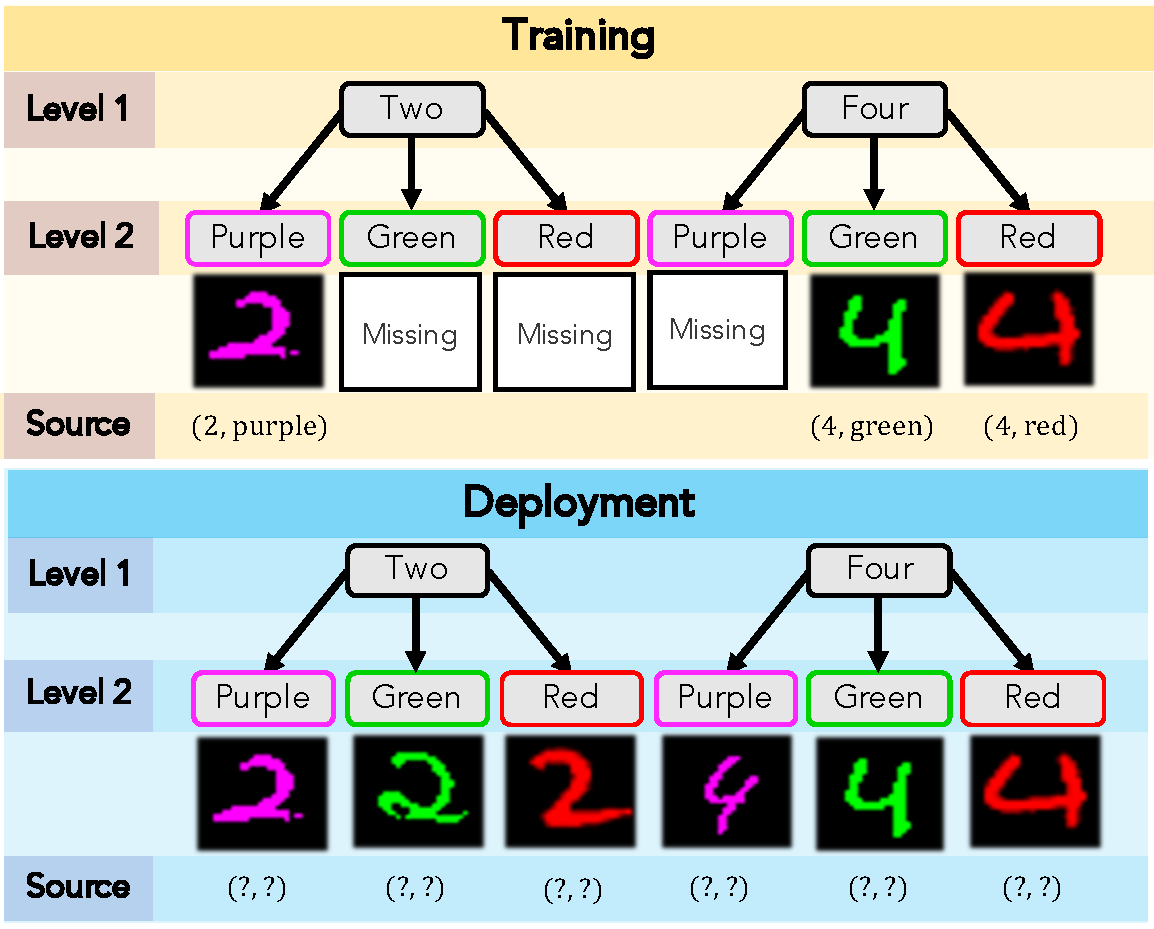
\includegraphics[width=0.7\columnwidth]{supmatch/figures/illustrations/problem_setup.pdf}
    \caption{%
      Illustration of our general problem setup. 
      %
      We assume the data follows a two-level hierarchy in which the first level corresponds to the class-level information (digit) and the second level corresponds to subgroup-level information (color).
      %
      While all digits appear in the training set (Top), not all digit-color combinations (sources) do; these gaps in conditional support give rise to a spurious correlation between digit and color, where the former is completely determined by the latter in the training set (giving the mappings $\textrm{{\color{purple}purple}} \rightarrow \texttt{2}$ and $\textrm{{\color{green}green}} \lor \textrm{{\color{red}red}} \rightarrow \texttt{4}$ as degenerate solutions to the classification problem), yet this same correlation does not hold for the deployment set (Bottom) which contains samples from the missing combinations.
      %
      To disentangle the (spurious) subgroup- and class-related information, we make use of an additional dataset that is representative of the data the model is expected to encounter at deployment time, in terms of the sources present.
    }%
    \label{fig:problem-setup}
\end{figure}


Machine learning has burgeoned in the last decade, showing the ability to solve a wide variety of
tasks with unprecedented accuracy and efficiency.
%
These tasks range from image classification \citep{krizhevsky2012imagenet} and object detection
\citep{ren2015faster}, to recommender systems \citep{ying2018graph} and the modelling of complex
physical systems such as precipitation \citep{ravuri2021skillful} and protein folding
\citep{jumper2021highly}.
%
In the shadow of this success, however, one finds less cause for optimism in frequent failure in
equitability and generalisation-capability, failure which can have serious repercussions in
high-stakes applications such as self-driving cars \citep{sun2019unsupervised}, judicial
decision-making \citep{mayson2018bias}, and medical diagnoses \citep{albadawy2018deep}.
%
ML's data-driven nature is a double-edged sword: while it opens up the ability to learn patterns
that are infeasibly complex for a practitioner to encode by hand, the quality of the solutions
learned by these models depends primarily on the quality of the data with which they were trained.
%
If the practitioner does not properly account for this, models ingesting data ridden with biases
will assimilate, and sometimes even amplify, those biases.
%
The problem boils down to not having sufficiently diverse annotated data, however collecting more
labelled data is not always feasible due to temporal, monetary, legal, regulatory, or physical
constraints.

%
While data can be intrinsically biased (such as in the case of bail records),
\emph{representational bias} is more often to blame, where socioeconomic or regulatory factors
resulting in certain demographics being under- (or even un-) represented. 
%
Clinical datasets are particularly problematic for ML due to the frequency of the different
outcomes being naturally highly imbalanced, with the number of negative cases (\texttt{healthy})
typically greatly outweighing the number of positive cases (\texttt{diseased}); even if a subgroup
is well-represented overall, that may well not be the case when conditioned on the outcome.
%
Equally, it is entirely possible that certain subgroups may be completely absent. 
%
For example, pregnant women are often excluded from clinical trials due to safety concerns, and if
they do participate it is often at too low a rate to be meaningful \citep{afrose2021overcoming}.

Like many prior works
\citep{SohDunAngGuetal20,kim2019learning,creager2021environment,SagRagKohLia20}, we consider
settings where there is a two-level hierarchy, with the second level partitioning the data into
\emph{subgroups} that are causally independent of the class (constituting the first level) which is
being predicted. 
%
This second level of the data is assumed to be predictable by the classifiers in the considered
hypothesis class. 
%
In both \citet{SohDunAngGuetal20} and \citet{creager2019flexibly} the entailed subgroups are
unobserved and need to be inferred in a semi-supervised fashion. We consider a similar problem but
one where the second level is partially observed.
%
Specifically, we focus on problems where some outcomes are available for some subgroups and not for
others. 
%
This particular form of the problem has -- so far as we are aware -- been hitherto overlooked
despite pertaining to a number of real-world problems.

%
If the labelled training set is sufficiently balanced in terms of classes and subgroups, a standard
ERM (empirical risk minimisation) classifier can achieve good performance.
%
However, we consider the added difficulty that, in the labelled training set, some outcomes
(classes) are not observed for all subgroups, meaning some of the classes do not overlap with all
the subgroups.
%
In other words, in the training set, some of the classes have \emph{incomplete support} with
respect to the subgroup partition, while in the deployment setting we expect all possible
combinations of subgroup and class to appear.
%
We illustrate our problem setup in Fig.~\ref{fig:problem-setup}, using Coloured MNIST digits as
examples; here, the first level of the hierarchy captures digit class, the second level, colour. 
%
While the (unlabelled) deployment set contains all digit-colour combinations (or \emph{sources}),
half of these combinations are missing from the (labelled) training set. 
%
A classifier trained using only this labelled data would wrongly learn to classify \texttt{2}s based
on their being {\color{purple}purple} and \texttt{4}s, based on their being {\color{green}green} or
{\color{red}red} (instead of based on shape) and when deployed would perform no better than random
due to the new sources being coloured contrary to their class (relative to the training set).

We address this problem by learning representations that are invariant to subgroups and that thus
enable the model to ignore the subgroup partition and to predict only the class labels.
%
In order to train an encoder capable of producing these representations, the information contained
in the labelled training set alone is not sufficient to break the \emph{spurious correlations}.
%
To learn the ``correct'' representations, we make use of an additional unlabelled dataset with
support equivalent to that of the deployment set (which includes the possibility of it being the
actual deployment set).
%
We do not consider this a significant drawback as such data is almost always far cheaper and less
labour-intensive to procure than \emph{labelled} data (which may require expert knowledge).
%

This additional dataset serves as the inductive bias needed by the encoder to disentangle class-
and subgroup-related factors.
%such that a downstream predictor can be trained using the available labels without risk of
%internalizing the spurious correlations present in the original data.
%
The encoder is trained adversarially to produce representations whose source (\texttt{training} or
\texttt{deployment}) is indeterminable to a set-classifier.
%
To ensure subgroup- (not class-) invariance is learned, the batches fed to the discriminator need
to be approximately balanced, such that they reflect the support, and not the shape, of the
distributions. 
%
We propose a practical way of achieving this based on semi-supervised clustering.
%

We empirically show that our proposed method can effectively disentangle subgroup and semantic
factors on a range of classification datasets and is robust to noise in the bag-balancing, to the
degree of outperforming the baseline methods even when no balancing of bags from the deployment set
is performed.
%
Furthermore, we prove that the entailed objective is theoretically guaranteed to yield
representations that are invariant to subgroups and that we can bound the error incurred due to
imperfect clustering.



\section{Problem setup}
\label{sec:problem-setup}
% -------------------------------------------------------------------------------
In this section, we illustrate and formalise the problem of classes with incomplete
subgroup-support. 
%
We start by defining requisite notation for conveying our setup and in
\S\ref{ssec:problem_formalism} expand on this notation to construct a more general and compact
description of said problem. 
%
Let \( x \in \gX \subset \R^d \), \( y \in \gY \) and \( s \in \gS \) denote the observed input
features, class labels and subgroup labels, respectively, with \( \gY \) and \( \gS \) being
non-empty, finite sets (i.e.\ \( \gY, \gS \in \{ A | A \in \gP(V), A \neq \varnothing, |A| <
\aleph_0 \} \)), and with upper-case letters denoting observed variables' random-variable
counterparts here (\(X\), \(Y\), and \(S\)) and throughout.
% the set-builder notation S = {A | A ∈ P(X), A ≠ ∅, |A| < ∞} defines the set of all non-empty,
% finite sets that are subsets of the set X.
%
We refer to the values, \( g \in \gG \) as \emph{sources}, representing unique pairs of \( s \) and
\( y \), such that \(  \gG \subseteq \gS \times \gY \). 
%
As in a standard supervised learning task, we have access to a labelled training set \( \gD^{tr}
\triangleq \{ (x_n, s_n, y_n) \}_{n=1}^{N^{tr}} \subset (\gX \times \gS \times \gY) \), that is used to
train a classifier \( \Gamma:\gX \rightarrow \gY \) that is then deployed on test set \( \gD^{te}
\triangleq \{ (x_n, s_n, y_n) \}_{n=1}^{N^{te}} \subset (\gX \times \gS \times \gY) \). 
%
We use superscript, to denote association of a domain with a correspondingly superscripted dataset,
e.g.\ \( \gG^{tr} \) and \( \gG^{te} \) respectively denote the sources in the training and test
sets.
%
Lastly, for some functions, we abuse notation and allow the random and observed variables to be
interchanged as inputs; we presuppose such functions (and their domain) are Borel measurable and
thus preserve the type of variable, i.e.\ a function of a random variable is also a random
variable.
%
For example, given function \(f: \gX \to \R \), we may write both \( f(x) \) and \( f(X) \),
meaning by the latter \( f \circ X(\omega) \) for some event \( \omega \in \Omega \).
%
% -------------------------------------------------------------------------------
\subsection{Spurious correlations from missing sources}\label{ssec:walkthrough}
% -------------------------------------------------------------------------------
The spurious correlation (\ac{SC}; \citealp{arjovsky2019invariant}), or shortcut-learning
\citep{valle2018deep, geirhos2020shortcut}, problem is characterised by the presence of some
secondary attribute \(s\) (such as background \citep{beery2018recognition}, texture
\citep{geirhos2018imagenet}, or gender \citep{sagawa2019distributionally, seyyed2020chexclusion}
that confounds the prediction task.
%
We refer to this attribute as the ``subgroup'', in line with algorithmic fairness (\ac{AF};
\citet{barocas-hardt-narayanan}) that is strongly correlated with the target attribute, \(y\), in
the training set, but spuriously so in the sense that the correlation the mapping \( \gS \to \gY \)
is acausal and thus cannot be expected to hold at deployment time. 
%
This correlation is pernicious when \(S\) is of lower complexity (which can be formalised in the
Kolmogorov sense; \citet{scimeca2021shortcut}) than the causal cues contained in \(X\), and thereby
becomes the preferred cue by virtue of simplicity bias \citep{valle2018deep}. 
%
Such problems have garnered considerable attention in recent years \citep{liu2021just,
pezeshki2021gradient, SohDunAngGuetal20, krueger2021out} due to their pervasive, and potentially
catastrophic \citep{codevilla2019exploring, de2019causal, castro2020causality}, nature.
%
In this paper, we introduce, and propose a semi-supervised solution for, a hierarchical and
class-asymmetric variant of the \ac{SC} problem that we term the \emph{\acf{MS}} problem .

To illustrate the general \ac{SC} problem and the \ac{MS} problem as a particular instantiation of
it, we define the conditional-probability matrix, \( \mathbf{P}^{tr} \in [0, 1]^{|\gS| \times
|\gY|} \), where each element \( \mathbf{P}^{tr}_{ij} \) encodes the conditional probability \(
P^{tr}(Y=j|S=i) \) in the training set, \( \gD^{tr} \). 
%
When \( \mathbf{P}^{tr} \) is both binary and doubly stochastic (that is, has all rows and columns
summing to 1) we have that \(y\) is completely determined by \(s\) in \( \gD^{tr} \) -- this is an
extreme form of the \ac{SC} problem which is statistically intractable without access to additional
sources of data \citep{KehBarThoQua20} or multiple environments \citep{arjovsky2019invariant}. 
%
The \ac{MS} problem can be viewed as a relaxation of this \ac{SC} wherein the elements of \(
\mathbf{P}^{tr} \) respect the constraint that all columns contain at least one non-zero value,
i.e.\ we observe all class labels but not all possible pairs of class and subgroup labels -- we say
that we have \emph{missing sources}, \(\gM\ \triangleq \gG^{te} \setminus \gG^{tr}\). 
%
This setup still leads to spurious correlations but ones that are statistically tractable due to
asymmetry.
%
Practically speaking, considering only cases where sources are entirely missing is overly
restrictive, and as such we instead view the problem setup as extending to cases where sources may
not be altogether missing but have sample sizes too small to constitute meaningful supervision. 
%
To understand the non-triviality of this problem, and why aiming for invariance to \(s\) in the
training set alone -- as is characteristic of many representation-learning methods in \ac{AF}
\citep{edwards2015censoring, madras2018learning, quadrianto2019discovering}  and domain adaptation
(\ac{DA}; \citep{ganin2016domain, zhao2018adversarial, saito2018maximum, lee2019sliced}) -- will
assuredly fail, consider a binary classification problem with binary subgroups, where \(\gY = \{ 0,
1 \}\) and \( \gS = \{ 0, 1 \}\) and for which \( \mathbf{P}^{tr} \) takes the form
%
\begin{align}\label{ms_example}
  \mathbf{P}^{tr} = \bordermatrix{
  & Y=0 & Y=1 \cr
  S=0 & 0.5 & 0.5 \cr
  S=1 & 1.0 & 0.0}~.
\end{align}
%
This represents a special case of the \ac{MS} problem that we refer to as the \emph{Subgroup Bias}
(SB) problem, distinguished by the fact that we observe all subgroups. 
%
Here, we have samples from $S=0$ evenly distributed across both the negative and positive classes;
for $Y=1$, however, we only observe samples from the negative class. 
%
This setup might appear somewhat benign at first blush, given that all classes are present in the
training set, however, the fact that \(s\) serves as a proxy for \(y\) in the case of $S=1$
frustrates our goal of subgroup-invariant classification. 
%
The reason for this becomes obvious when decompose a classifier into a mixture of experts (MoE),
where \(s\) indicates which expert to choose for the given sample. 
%
Such a model naturally arises in practice due to the tendency of deep neural networks to strongly
favour shortcut solutions \citep{geirhos2020shortcut}.
%
We note that for this, and throughout the paper, we assume that \(s\) is inferable, to some extent,
from $x$, that is \( \gI(X; S) > 0 \), with \( \gI(\cdot; \cdot) \) denoting the mutual information
between two variables -- this is almost always the case in practice but we make the dependence
explicit here by denoting by \( X_Y \) the causally-relevant component of \( X \)), that is
independent of \(S\), and by including \( s \in \{0, 1\} \) explicitly in the set of inputs.
%
With this noted, we may then define the MoE classifier, \(c_{MoE}\), that `solves' the training set
with labels distributed according to \( \mathbf{P}^{tr} \) as
%
\begin{align}
  c_{MoE}(X_Y, S) = \begin{cases}
c_{S=0}(X_Y) &S=0 \\
0 &S=1 \\
\end{cases},
\end{align}
%
using \(c_{S=0}(\cdot)\) to denote the expert that learns to classify only the subset of the data
for which $S=0$.
%
Such a classifier is clearly undesirable, as should it ever encounter a sample belonging to
subgroup $1$ with a positive label, the classifier will automatically declare it negative without
needing to attend to $X_Y$ -- it is invariant to $X_Y$ while being variant to \(S\), which is the
opposite of what we desire. 
%
This is often done by learning an encoder $f: \gX \to \gZ$ that maps an input $x$ into a
representation, \( z \in \gZ \subset \R^l \), which has the desired property of \(S\)-invariance,
\( Z \perp S \), while also maximising $\gI(Z; Y)$ so that the representation is useful for
classification. 
%
A popular way of imparting this invariance is with adversarial methods \citep{ganin2016domain,
zhao2018adversarial, madras2018learning} where  $f$ is trained to the equilibrium point, $f^\ast$,
of the (non-convex) minimax equation 
%
\begin{align}\label{eq:moo}
\underset{f \in \gF}{\text{min}}\; \underset{a \in \gA}{\text{max}}\,
\E_{(x, s, y) \sim \gD^{tr}}
\big[ 
  \textcolor{red}{ \overbrace{ a(f(x))_s }^{ \text{invariance}} }
  - \textcolor{blue}{ \underbrace{ \lambda \gI(f(x); y) }_{ \text{classification} } }
\big],
\end{align}
%
where \( a: \gZ \to \bigtriangleup^{|\gS|} \) is a parametric adversary with codomain the standard
simplex over \( \gS \), and \(\lambda \in \R^+\) is a positive scalar controlling the trade-off
between the two constituent objectives. 
%
Under ideal conditions, when all possible pairs of \(s\) and \(y\) are observed, \(f^\ast\)
corresponds to the point at which \(a\) is maximally entropic and occurs when \(Z\) is invariant to
\(S\), and only \(S\), while mutual information \wrt{} \(Y\) is jointly maximised -- from an
optimisation standpoint, the gradients of first and second objectives are non-conflicting (i.e.\
have non-negative inner products; \citealp{yu2020gradient}) and there is no trade-off. 
%
However, in cases where we have missing sources, the waters are muddied: satisfying the first part
of the objective connotes invariance not only to \(S\), but also to \(Y\), since \(S\) can be
predicted from \(Y\) with above-random accuracy due to the skewed statistics of the dataset. 
%
This is patently problematic as \(Y\) is the very thing we wish to predict and achieving invariance
to \(S\) does little good if our classifier can no longer utilise features predictive of \(Y\). 

Since we cannot achieve optimality for the competing invariance and classification terms
simultaneously, we instead have a set of \ac{PO} solutions that collectively make up the Pareto
front -- learning the solutions corresponding to different trade-offs, or preference vectors, is
the domain of \acl{MOO} (\acs{MOO}; \citealp{deb2014multi}). 
%
Specifically, Eq.~\ref{eq:moo}, with \(\lambda\) controlling the preference direction,
characterises the most straightforward approach to MOO, called \emph{linear scalarisation}
\citep{boyd2004convex}. 
%
\Ac{MOO} has recently been explored in the context of \ac{UDA}, for controlling the descent
direction, in unsupervised domain adaptation (UDA) in light of the conflict arising between the
gradients of the alignment and classification terms \citep{liang2021pareto}, and in \acf{AF} for
controlling the inherent trade-off between predictive performance and fairness (typified by the
\emph{Accuracy-Fairness trade-off}; \citet{martinez2020minimax}).
%
While our missing-sources problem admits a \acs{MOO}-based approach, we are instead interested in
leveraging unlabelled data to sidestep the implied trade-off altogether.
% -------------------------------------------------------------------------------
\subsection{Formalising the problem}\label{ssec:problem_formalism}
% -------------------------------------------------------------------------------
In order to provide a general formulation of the \ac{MS} problem exemplified above, we begin by
defining additional notation for reasoning over label-conditioned subsets and their support. 
%
For a given dataset, \( \gD \), we denote by \( \gD_{S=s^\prime} \) its subset with subgroup label
\( s^\prime \in \gS \), by \( \gD_{Y=y^\prime} \) its subset with class label \( y^\prime \in \gY
\), and -- combining the two -- by \( \gD_{S=s^\prime,Y=y^\prime} \) its subset with subgroup label
\( s^\prime \) and class label \( y^\prime \).
%
According to this scheme, \( \gD_{S=\text{\color{purple}{purple}}, Y=\text{2}} \) should then be
read as ``the set of all samples in \( \gD \) with class label `2' and subgroup label
`\textcolor{purple}{purple}'''.
%
We apply similar syntax to the subgroups, writing \( \gS^{tr}_{Y=y^\prime} \) to mean the observed
subgroups within class \(y\) in the training set.
%
For instance, \(\gS^{tr}_{Y=1}=\{0\}\) prescribes that for class \(1\), only subgroup \(0\) is
present in the training set.

We assume a problem of a hierarchical nature.
%, as illustrated in Fig.~\ref{fig:problem-setup}. 
%
While the full set of class labels is observed in both the training and test sets, we do not
observe all pairs of \(s\) and \(y\) in the former, i.e.\ \( \gG^{tr} \subset \gG^{te} \) or \(\gM
\neq \varnothing \). 
%
Equivalently, we say that for some class, \(y^\dagger\), we have \( \gS^{tr}_{Y=y^\dagger} \subset
\gS \), subject to the constraint that \(  \gS^{tr} = \gS^{te} \).
%
With this, we can succinctly notate the SB problem realised by Eq.~\ref{ms_example}, in which class
\(Y=1\) has no overlap with subgroup \(S=1\), as \(\gS^{tr}_{Y=1}=\{0\}\) (while
\(\gS^{tr}_{Y=0}=\{ 0, 1 \}\)), corresponding to \( \gM = \{(1, 1)\} \), and distinguish SB
problems generally by the inclusion of the additional constraint \( \gS^{tr} = \gS^{te} \).
%
To illustrate a more complex case, the SB problem depicted in Fig.~\ref{fig:problem-setup}, in
which for we observe exclusively purple `2's and green and red `4's, can be notated with the pair
\( \gS^{tr}_{Y=2}=\{\text{\textcolor{purple}{purple}\}} \), \( \gS^{tr}_{Y=4}=\{
\text{\textcolor{green}{green}}, \text{\textcolor{red}{red}} \} \).
% -------------------------------------------------------------------------------
\subsection{A way forward}
% -------------------------------------------------------------------------------
In this paper, we propose to alleviate the SB problem by mixing labelled data with
\emph{unlabelled} data that is usually much cheaper to obtain \citep{ChaSchZie06}, referring to
this set of \emph{unlabelled} data as the \emph{deployment set} 
%
\footnote{In our experiments, we report accuracy and bias metrics on another independent test set
instead of on the unlabelled data that is available at training time.} \( \gD^{dep}_\star =\{(x_n,
s_n^\star, y_n^\star)\}_{n=1}^{N^{dep}} \subset (\gX \times \gS \times \gY) \), using ``\(\star\)''
to denote that the labels are \emph{unobserved}, and in practice we only have access to \(
\gD^{dep} \triangleq \{(x_n)\}_{n=1}^{N^{dep}} \subseteq \gX \) and must estimate the corresponding
sources.
%
We assume that this deployment set is source-complete \wrt{} the test set, \( \gG^{dep} = \gG^{te}
\). Leveraging this deployment set, we seek to learn a classifier, \( \Gamma \), that can
generalise well to the missing sources appearing in the test set without seeing any labelled
representatives in the training set. 
%
In practice, we treat \( \Gamma \) as a composition, \( c \circ f \), of two subfunctions: an
encoder \( f: \gX \to \gZ \), which maps a given input \( x \) to a representation \( z \in \gZ
\subseteq \R^l \), and a classifier head \( c: \gZ \to \gY \) which completes the mapping to the
space of class labels, \( \gY \). 
%
Since the task of achieving independence between the predictions and subgroup labels can be reduced
to the task of learning the invariance \( Z \perp S \); we next discuss how one can learn an
encoder satisfying this condition in a theoretically-principled manner.
% -------------------------------------------------------------------------------
% % ********************************************************************************
\section{Some notes on notation}\label{sec:notation}
% ********************************************************************************
We describe here some of the general notation schemes used throughout this background chapter,
leave the concrete notation to be defined contextually, both to allow overloading (to allow for
reuse and restrictedness of the alphabet) and to minimise cognitive overhead for the reader.

%
First, we denote random variables using upper-case (non-calligraphic) letters and their associated
observed/deterministic/realised variables with the corresponding lower-case letters.
%
Following convention, we consistently denote by \(X\) and \(Y\) the input (covariate) and
target (response) variables, respectively; by \(S\) some auxiliary variable on which we want to
condition (for evaluation and/or optimisation), such as the domain (in domain
adaptation/generalisation) or sensitive attribute (in algorithmic fairness); by \(Z\) the latent
space, representations, encodings, or embeddings (all synonymously) of some model.
%
Second, calligraphic letters are used to denote (but not exclusively) the domain of a variable,
e.g. \(x \in \gX \).
%
Under this scheme, we would have for the random variable, \(X: \Omega \to \R^d \), realisations \(x
\in \gX \subset \R^d \) defined on a subset of the \(d\)-dimensional space of real numbers.
%
We then use \(P(\cdot)\) to denote probability distributions with conditioning indicated as
\(P(X=x)\) -- continuing the foregoing example -- and use \(\gD\) to denote \emph{datasets} that
correspond to the empirical distributions of variables; for instance \(\gD \triangleq
\{x_i\}_{i=1}^N \) denotes a dataset made up of \(N\) observations of \(X\).
%
We will often augment this notation with super- and subscripts to indicate a variety of concepts
including, inter alia, association with a particular subset of the data or concept, optimality,
observability, and approximation.
%
Some representative examples include \(\gD^{tr}\) and \(\gD^{te}\) to denote the training and test
sets, respectively, \(f^\ast\) to denote the optimal function \wrt{} some optimisation problem, and
\(\hat{y}\) to denote a prediction made by some estimator (of \(P(Y|X)\)).
%
% We will state the exact meaning in each case, whenever it is not obvious by association.

%
Finally, to simplify exposition, we abuse notation by allowing functions of the form \(f: X \to Y
\) to accept random and observed variables interchangeably; we assume that the derived function
classes are Borel Measurable and as such that a function of a random variable is also a random
variable. \(f\) to operate on random variables \(X\).
% %
Thus, pedantically speaking, \( f(X) \) should be read as shorthand for \( f \circ X(\omega) \),
for some event \( \omega \) drawn from sample space, \( \Omega \), while \( f(x) \) should be read
in the standard fashion, with deterministic inputs and outputs.



\section{Adversarial Support-Matching}
\label{sec:adversarialsm}
\begin{figure*}[tb]
  \centering
  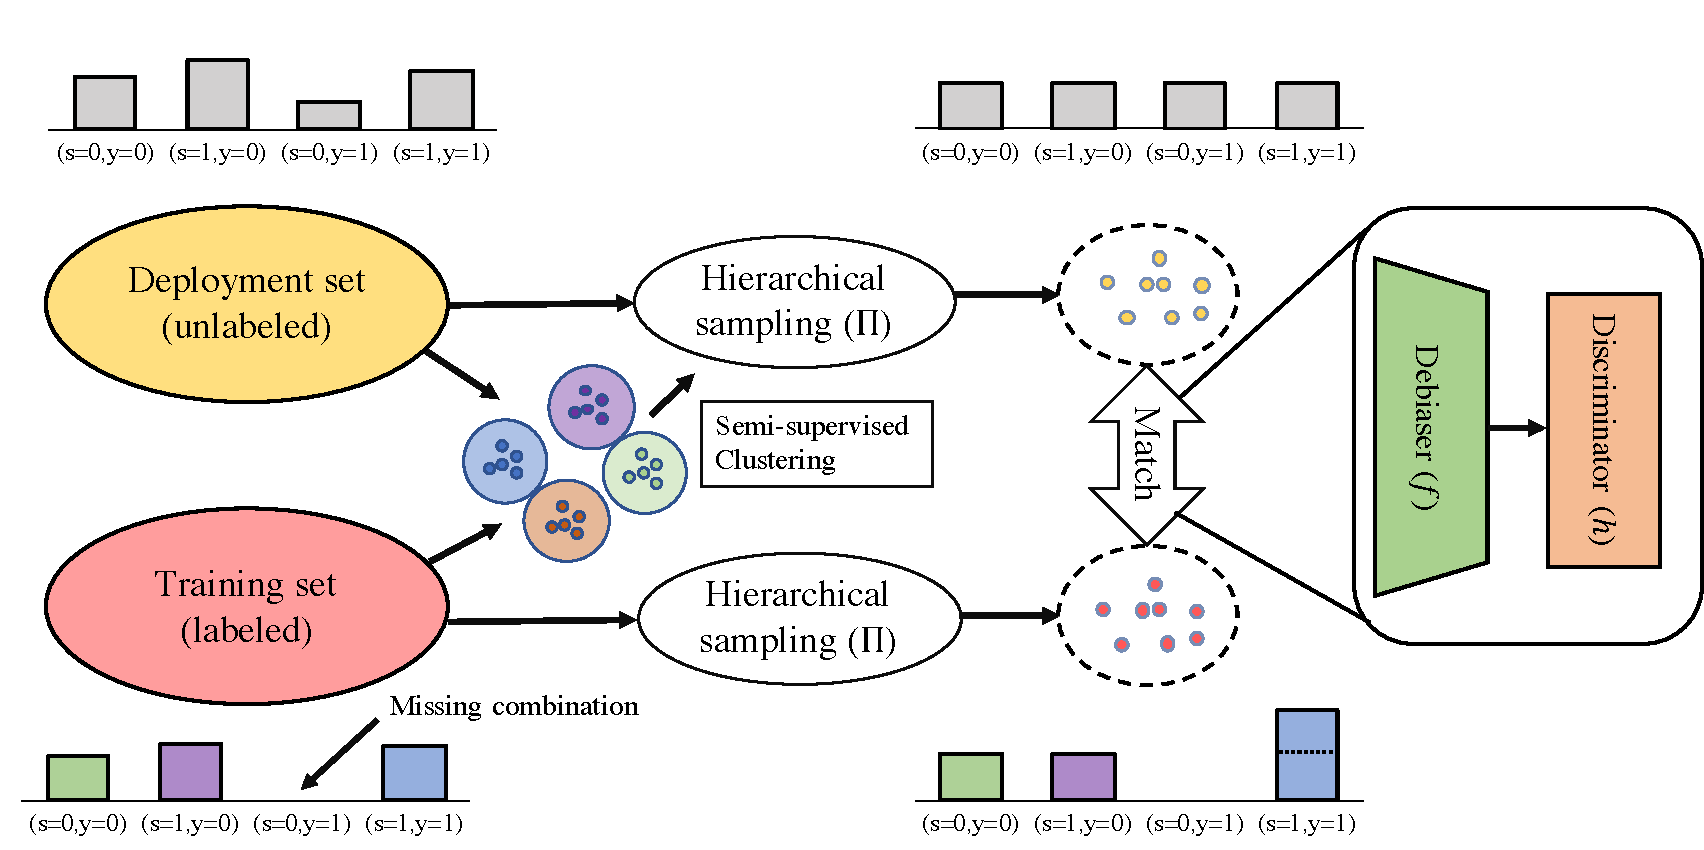
\includegraphics[width=1.0\textwidth]{supmatch/figures/illustrations/pipeline.pdf}
  \caption{%
    Visualisation of our support-matching pipeline.
    % A source is defined as certain combinations of the subgroup, s, and target class, y. Bags are
    % sampled from one of two datasets. The training set has labeled information about both $s$ and
    % $y$ but may be missing support over $S\times Y$. The deployment set on the other hand, is
    % assumed to have full support over $S \times Y$ but is unlabeled, meaning it cannot be used
    % for directly training a classifier. 
    Bags are sampled from the training and deployment sets using the hierarchical sampling
    procedure described in \S\ref{sec:sm-adversarialsm} and defined functionally in
    Eq.~\ref{eq:functional-sampling}. 
    %
    Since we cannot use ground-truth labels for hierarchical sampling of the deployment set, we use
    a semi-supervised clustering algorithm to produce balanced batches. In the event that certain
    combinations are missing, as shown here for $(s=0,y=1)$, the sampling on the training set
    substitutes the missing combinations with combinations that ensure equal representation of the
    target classes. 
    %
    The debiaser is adversarially trained to produce representations from which the source dataset
    cannot be reliably inferred by the discriminator. 
    %
    Assuming the bags are sufficiently balanced and $\gG^\mathit{tr}  \subsetneq \gG=\gS\times\gY$,
    the optimal debiaser is one that produces a representation $z$ that is invariant to $s$, which
    we prove in Appendix~\ref{implication-of-the-objective}.
    }%
  \label{fig:sm-pipeline}
\end{figure*}



We cast the problem of learning a subgroup-invariant representation as one of
\emph{support-matching} between a dataset that is \emph{labelled} but has \emph{incomplete} support
over sources, $G$, and one, conversely, that has \emph{complete} support over $G$, but is
\emph{unlabelled}. 
%
The idea is to produce a representation that is invariant to this difference in support, and thus
invariant to the subgroup. However, it is easy to learn the wrong invariance if one is not careful.
% Simply matching the distributions of the two datasets would wrongly result in the relative
% frequency of the sources being taken into account and the potential loss of task-relevant
% information.
To measure the discrepancy in support between the two distributions, we adopt an adversarial
approach, but one where the adversary is operating on small sets -- which we call \emph{bags} --
instead of individual samples. 
%
%
%
These bags need to be balanced with respect to ($s$, $y$), such that we can interpret them as
approximating $\gG$ as opposed to the joint probability distribution, $P(S, Y)$.
%
Details on how these bags are constructed can be found in in \S\ref{ssec:sm-realisation} and
\S\ref{sec:sm-implementation}.
% These sets correspond to the "perfect bags" introduced in the next section,
% \S\ref{ssec:perfect-bags}:


\subsection{Objective}\label{ssec:sm-objective}
%
We now present our overall support-matching objective. 
%
As alluded to before, the goal, in summary, is to learn an encoder, \(f\), which
preserves all information relating to $Y$, but is invariant to $S$. 
%if the training set is incomplete \wrt{} $s$.
Let \(P^{tr}(f(X)=z', S=s',Y=y')\) be the joint probability that a data point \(x\) drawn
from \(P^{tr}(X)\) -- the training set -- results in the encoding \(z'\) and is at the same
time labelled as subgroup \(s'\) and class \(y'\). 
%
We also define the following shorthand: $p_f(Z=z')=P^{tr}(f(X)=z')$, the distribution
resulting from sampling \(x\) from \(P^{tr}\) and then transforming \(x\) with \(f\).
%
Analogously for the deployment set: $q_f(Z=z')=P^{dep}(f(X)=z')$. 
%
For the conditioned distributions we write $p_f|_{S=s',Y=y'}$, following the convention established
in \S\ref{ssec:problem_formalism} but with the added `\(|\)' to clearly delimit the
conditioning.

The objective makes a distinction between those classes, \(y \in \gY\), for which there is overlap
with all subgroups \(s \in \gS\) in the training set and those classes for which there is not.
% An extreme version of this is when \emph{none} of the classes have overlap with a specific subgroup.
% In the \emph{missing subgroup} scenario, \emph{none} of the classes have overlap with all subgroups \(s\).
To formalise this, we define the following helper function $\Pi$ which maps \((s',y')\) to a set of
subgroup identifiers depending on whether the class \(y\) has full \(s\)-support:

\begin{align}\label{eq:Pi}
\Pi(s',y') = \begin{cases}
  \{s'\}&\text{if }\,\gS^{tr}_{ Y=y' }=\gS \\
  \gS^{tr}_{ Y=y' }&\text{otherwise.}
\end{cases}
\end{align}
%
$\Pi(s,y)$ ensures that the correct invariance is learned and is discussed in more detail further below.
Our objective is then
%
\begin{align}
  \gL_\text{match}(f)=\sum\limits_{s'\in\gS}\sum\limits_{y'\in\gY} d(p_f|_{s\in \Pi(s',y'),Y=y'},
  q_f|_{S=s',Y=y'})
\label{eq:objective}
\end{align}
%
where \(d(\cdot, \cdot)\) is a distance measure for probability distributions.
The optimal encoder $f^*$ is found by solving the following optimisation problem:
%
\begin{align}
  f^*=
  \argmin\limits_{f\in\gF} 
  \textcolor{red}{
  \gL_\text{match}(f)
  }
  - 
  \textcolor{blue}{
  \gI(f(X);X)
  }
\end{align}
%
where $\gI(\cdot; \cdot)$ again denotes the mutual information. As written, Eq.~\ref{eq:objective}
requires knowledge of \(s\) and \(y\) on the deployment set for conditioning. 
%
That is why, in practice, the distribution matching is not done separately for all combinations of
\(s'\in\gS\) and \(y'\in\gY\). 
%
Instead, we compare \emph{bags} that contain samples from all combinations in the right
proportions. For the deployment set, Eq.~\ref{eq:objective} implies that all
\(s\)-\(y\)-combinations have to be present at the same rate in the bags, but for the training set,
we need to implement \(\Pi(s',y')\) with hierarchical balancing.

As the implications of the given objective might not be immediately clear,
we provide the following proposition.
%
The proof can be found in Appendix~\ref{sec:sm-theoretical-analysis}.
%
\begin{theorem}
%
If \(f\) is such that
%
\begin{align}
p_f|_{s\in \Pi(s',y'),Y=y'} = q_f|_{S=s',Y=y'}\quad\forall s'\in\gS, y' \in\gY
\end{align}
%
and \(P^{tr}\) and \(P^{dep}\) are data
distributions that correspond to the real data distribution \(P\),
except that some \(s\)-\(y\)-combinations are less prevalent, or, in the
case of \(P^{tr}\), missing entirely, then, for every
\(y' \in \gY\), there is either full coverage of \(s\) for \(y'\)
in the training set (\( \gS^{tr}_{ Y=y' }=\gS \)), or the
following holds:
%
\begin{align}
P(S=s'|f(X)=z', Y=y')=\frac{1}{n_s}~.
\end{align}
%
In other words: for \(Y=y'\), \(f(x)\) is not predictive of \(s\).
\end{theorem}

\subsection{Implementation}\label{ssec:sm-realisation}
%
The implementation of above objective combines elements from unsupervised representation-learning and
adversarial learning.
% For simplicity, we follow an autoencoder paradigm for the former but any
% unsupervised/self-supervised representation learning objective could be used in place of the
% reconstruction objective.
In addition to the invariant representation $z$, our model also outputs $\tilde{s}$, in a similar
fashion to \citet{KehBarThoQua20} and \citet{creager2019flexibly}. 
%
This can be understood as a reconstruction of the subgroup information from the input $x$ and is
necessary to prevent $z$ from being forced to encode $s$ by the reconstruction loss.
%
We note that this need could potentially be obviated through use of self-supervised approaches,
but refrain from exploring this avenue in the interest of simplicity.

The model, \(\Gamma\), is composed of three core modules: 
1) two \emph{encoder} functions, $f$ (which we refer to
as the ``debiaser'') and $t$, which share weights and map $x$ to $z \in \gZ$ and
$\tilde{s} \in \tilde{\gS}$, respectively;
2) a \emph{decoder} function \(r: \gZ \times \tilde{\gS} \to \gX\) that learns to
invert $f$ and $t$; and
% 3) \emph{predictor} functions $\ell_y$ and $\ell_s$ that predict $y$ and $s$
% from $z$ and $\tilde{s}$ respectively, and
3) a \emph{discriminator} function \( h: (\mathfrak{Z} \subseteq \gP(Z)) \to ( 0, 1 ) \) that
predicts which dataset a bag of samples, \(\gB\ \in \mathfrak{Z}\), embedded in $\gZ$, was sampled
from, where we have used \( \gP(\cdot) \) to denote the powerset of its argument and thereby a
domain comprising sets of elements of \(\gZ\).
% The predictor $\ell_s: \tilde{\gS} \to \bigtriangleup^{|\gS|}$ (with $\bigtriangleup^{|\gS|}$
% denoting the $|\gS|$-dimensional standard simplex) is usually the identity function, and is
% primarily listed here for notational symmetry. Fig. \ref{fig:architecture} illustrates how $f$
% and $h$ interact during training -- the decoding step involving the other two components, $t$ and
% $g$, is omitted for compactness. This marks a significant departure from the typical GAN
% discriminator, which takes as input batches of data and yields a prediction for each sample
% independently of the other samples in the batch. %, where the training signal comes from the
% perfect dataset.
%
The encoder $f$ is then tasked with learning a representation $z$ such that it is indeterminable to
the adversary $h$ whether a given bag originated from the deployment set (`positive') or the
training set (`negative').
Formally, given bags
\( \gB^{tr} \), sampled according to \(\Pi\) from the training set, and balanced bags from the deployment
set, \( \gB^\mathit{dep} \), we first define, for notational convenience, the loss \wrt{} to the
encoder networks, $f$ and $t$ as
%
\begin{align}
&\gL_\text{enc}(f, t, r, h) = 
  \sum_{b^{dep} \in \gB^{dep}}
  \sum_{b^{tr} \in \gB^{tr}} 
\textcolor{blue}{
  \Bigg[\,
    \overbrace{
    \sum_{x \in b^{dep} \cup b^{tr}} 
      \lVert x - r(f(x), t(x))\rVert_p^p}^{\gL_{\text{recon}}}
    \Bigg]
    }
    \nonumber\\
   &\quad\quad\quad\quad\quad\quad
 %   +  
   \textcolor{red}{
     \underbrace{ \lambda_\text{match}  \Bigg[
       \log h \bigl( \{ \texttt{sg}[f(x)]\ | x \in b^\mathit{dep} \} \bigr) 
       - \log h \bigl( \{ f(x)\ | x \in b^\mathit{tr} \} \bigr) 
 \Bigg] }_{\gL_{\text{match}}}
},
   % \nonumber\\
   % &\quad+ \!\!\sum_{x\in b_\mathit{tr}}
   % \lambda_y L_{\text{sup}} (
   % y, \ell_y(f(x))) + \lambda_s L_{\text{sup}} (s, \ell_s(t(x)))
\label{eq:disentangling}
\end{align}
%
where \( \gL_{\text{recon}} \) denotes the reconstruction loss defined by the \(p\)-norm (\(p=1\)
and \(p=2\) yielding MAE and MSE, respectively), \( \gL_\text{match} \) denotes the adversarial loss,
\( \lambda_\text{match} \in \mathbb{R}^+_\ast \) is a pre-factor controlling the trade-off between
the loss terms, and \( \texttt{sg}[\cdot] \) denotes the ``stop-gradient`` operator that behaves as
the identity function but with zero partial derivatives.
%
The overall objective, encompassing $f$, $t$, and $h$ can then be formulated in terms of
\( \gL_\text{enc} \) as
%
\begin{align}
    \underset{f, t, r}{\textrm{min}}\; \underset{h}{\textrm{max}}\,\gL_\text{enc}(f, t, h)~.
    \label{eq:disentangling_total}
\end{align}
%
This equation is computed over batches of bags and the discriminator is trained to map a bag of
samples from the training set and the deployment set to a binary label: $1$ if the bag is adjudged to
have been sampled from the deployment set, $0$ if from the training set.
% Its goal is to effectively estimate the probability that a bag of samples has been sampled from
% one distribution or the other.
For the discriminator to be able to classify sets of samples, it needs to be permutation-invariant
along the bag dimension -- that is, its predictions should take into account dependencies between
samples in a bag while being invariant to the order in which they appear. 
% We experiment with two different types of attention mechanism for the bag-wise pooling layer of our
% discriminator, finding them both to work well.
\corr{
To aggregate information over samples within the bags, we employ a self-attention-based
\citep{vaswani2017attention} pooling layer, with aggregation achieved simply by setting the query
vector to be the mean of the (projected) representations over the bag dimension.
%
For more details, see Appendix~\ref{ssec:attention-mechanism}. 
%
Furthermore, in Appendix~\ref{ssec:no-mil}, we validate that having the discriminator operate over
sets (bags) of samples rather than independent samples (with the same balancing scheme) is
essential for achieving good and robust (\wrt{} balancing quality) empirical performance,
though we note that the two realisations yield minimax objects with theoretically-equivalent optima.
%
This observation on the difference in stability between the two realisations may have implications
for adversarial training more broadly, however we focus on the much narrower scope of the \ac{MS}
problem and leave it to future work to explore such implications.
}
% CORRECTION: there was a discussion of bags somewhere in this chapter ( i got a bit lost!) but as
% per the discussion in the viva discuss the influence of bags. potentially could be something to
% say as future work. Also could mention the use of the mean as the query in the attention
% mechanism could be good. Discuss with novi if this is novel enough to warrant taking further

% Our goal is to make $z$ invariant to the subgroup $s$. However, what the adversarial loss
% actually enforces is that $z$ generates bags with the same support over $S \times Y$ irrespective
% of the dataset they were drawn from. To ensure that the disentangling aligns with our objective,
Our goal is to disentangle $x$ into two subspaces: a subspace $z$, representing the class, and a
subspace $\tilde{s}$, representing the subgroup.
%
For the problem to be well-posed, it is crucial that the bags differ only
in terms of which sources are present and not in terms of other aspects.
% with respect to the class-subgroup combinations present and not with respect to the shape of the
% underlying distribution.
We thus sample the bags according to the following set of rules which operationalize $\Pi$. Please
refer to Fig.~\ref{fig:sm-pipeline} for a visualisation of the effect of these rules. 
%
\begin{enumerate}\label{ls:rules}
  %
  \item Bags of the deployment set are sampled so as to be approximately balanced with
    respect to $s$ and $y$ (all combinations of $s$ and $y$ should appear in equal number). 
    %
  \item For bags from the training set, all possible values of $y$ should appear with equal
    frequency. Without this constraint, there is the risk of $y$ being encoded in $\tilde{s}$
    instead of $s$. 
  \item Bags of the training set should furthermore exhibit equal representation of each subgroup
    within classes so long as rule 2 is not violated.
    For classes that do not have complete $s$-support, the missing combinations of $(s, y)$ need to
    be substituted with a sample from the same class -- i.e., if $s \notin \gS^{tr}(y)$ we instead
    sample randomly from a uniform distribution over $\gS^{tr}(y$). 
    %
\end{enumerate}

% We supplement the implicit constraints carried by the balancing of the bags with the explicit
% constraint that $z$ be predictive of $y$, which we achieve using a linear predictor $\ell_y$.
% Whenever we have $\textrm{dim}(\mathcal{S}_{tr}) > 1$, %(in our experiments this corresponds to the
% \emph{subgroup bias} setting) we can also impose the same constraint on $\tilde{s}$, but with
% respect to $s$.

\algrenewcommand\algorithmicrequire{\textbf{Input:}}
\algrenewcommand\algorithmicensure{\textbf{Output:}}
\begin{algorithm}
  \caption{Adversarial Support Matching}\label{alg:cap} 
  \begin{algorithmic}
    \Require Number of encoder updates $N^\text{enc}$, number of discriminator updates $N^\text{disc}$,
    encoders $f$ and $t$, decoder $r$, discriminator $h$, training set $\gD^{tr}$, deployment set
    $\gD^{dep}$
    \Ensure Debiaser $f$ with learned invariance to $s$
    \\

    \For{$i \gets 1$ to $N^\text{enc}$} \Comment Encoder update loop
    \State Sample batches of perfect bags $\gB^{tr} \sim \gD^{tr}$ and $\gB^{dep} \sim
    \gD^{dep}$ using $\Pi$ (Eq.~\ref{eq:Pi})
    \State Compute $\gL^\text{enc}$ using Eq.~\ref{eq:disentangling_total}
    \State Update $f$, $t$, and $r$ by descending in the direction $\nabla \gL^\text{enc}$
    \For{$j \gets 1$ to $N^\text{disc}$} \Comment Discriminator update loop
    \State Sample batches of perfect bags $\gB^{tr} \sim \gD^{tr}$ and $\gB^{dep} \sim
    \gD^{dep}$ using $\Pi$ (Eq.~\ref{eq:Pi})
    \State Compute $\gL^\text{match}$ using Eq.~\ref{eq:disentangling_total}
    \State Update $h$ by ascending in the direction $\nabla \gL^\text{match}$
    \EndFor
    \EndFor

  \end{algorithmic}
\end{algorithm}

%
\subsection{Perfect bags}\label{sec:sm-implementation}
%
A visual overview of our pipeline is given in Fig.~\ref{fig:sm-pipeline}. 
%
Borrowing from the \ac{AF} literature \citep{chouldechova17,KleMulRag16}, we refer to a bag in
which all elements of $\gG$ appear in equal proportions as a ``perfect bag'' (even if the balancing
is only approximate). 
%
Our pipeline can be broken down into two steps: 1) sample perfect bags from an unlabelled
deployment set; and 2) produce disentangled representations using the perfect bags via adversarial
support-matching as described in \S\ref{ssec:sm-realisation}.

\textbf{Constructing perfect bags via clustering.}
%
We cluster the data points from the deployment set into \( N^C=|\gG| \) clusters by applying
spherical k-means to CLIP \cite{radford2021learning} (visual) embeddings. 
%
Specifically, we use the ResNet-50 version of CLIP, finding this to work better than the ViT-based
variants. 
%
We inject labelled knowledge into the k-means algorithm by initialising the centroids of the known
sources the mean of their features in the labelled (training) data. 
%
We find this works reasonably well for the considered datasets; since, the aim of this work is to
propose a pipeline for effectively leverage unlabelled data for invariance-learning, not to set a
new state-of-the-art in clustering, we adopt this simple clustering method for a practical
proof-of-concept compared with the artificial approach of injecting noise into the ground-truth
labels. 
%
The latter procedure is useful, however, for performing a fine-grained sensitivity analysis of our
algorithm \wrt{} clustering accuracy, in that we can simulate the runs of the algorithm at
different levels of noisiness in the bag-sampling. 
%
% We present such an analysis in \S\ref{ssec:sensitivity}.
%
Given, the cluster assignments, we can then stratify the deployment set into perfect bags, to be
used by the subsequent support-matching phase.

As a result of clustering, the data points in the deployment set \( \gD^\mathit{dep} \) are
labelled with cluster assignments generated by clustering algorithm, \( C \), giving \(
\gD^\mathit{dep}_C=\{(x_i, c_i)\} \), \(c_i = C(z_i) \),
%
so that we can form perfect bags from \( \gD^\mathit{dep}_C \) by sampling all clusters at equal
rates; there is no need for application of the $\Pi$ operator since the deployment set is complete
\wrt{} $\gG$.
%
We note that we do \emph{not} have to associate the clusters with specific $s$ or $y$ labels as the
labels are not directly used for supervision.

Balancing bags based on clusters instead of the true labels introduces an error, which we can try
to bound. 
%
For this error-bounding, we assume that the probability distribution distance measure used in
Eq.~\ref{eq:objective} is the \emph{total variation distance} \(TV\). 
%
The proof can be found in Appendix~\ref{sec:sm-theoretical-analysis}.

\begin{theorem}
%
If \(q_f(Z)\) is a data distribution on \(\gZ\) that is a mixture of \(n_y\cdot n_s\) Gaussians,
which correspond to all the unique combinations of \(y\in\gY\) and \(s\in\gS\), and \(p_f(Z)\) is
any data distribution on \(\gZ\), then without knowing \(y\) and \(s\) on \(q_f\), it is possible
to estimate
%
\begin{align}
  \sum\limits_{s^\prime\in\gS}\sum\limits_{y^\prime\in\gY} TV(p_f|_{s\in
  \Pi(s^\prime,y^\prime),Y=y^\prime},
q_f|_{S=s^\prime,Y=y^\prime})
\end{align}
%
with an error that is bounded by \(\tilde{O}(\sqrt{1/N})\) with high probability, where \(N\) is
the number of samples drawn from \(q_f\) for learning.
%
\end{theorem}
%

\subsection{Limitation and intended use}
\label{sec:sm-limitations}
% First, dataset consumers should take extra care about the cost-benefit analysis of selecting particular datasets for their machine learning tasks. 
%
Although having zero labelled examples for some subgroups is not uncommon due to the effects of
systematic bias or dataset curation, we should make a value-judgement on the efficacy of the dataset
with respect to a task.
%
% {\color{red}Corrective action such as the one described in this paper or inaction should be
% recorded.}
We can then decide whether or not to take corrective action as described in this paper.
%
A limitation of the presented approach is that, for constructing the perfect bags used to train the
disentangling algorithm, we have relied on knowing the number of clusters \emph{a priori},
something that, in practice, is perhaps not the case. However, for person-related data, such
information can, for example, be gleaned from recent census data. 
%
(see also Appendix~\ref{sec:sm-overclustering} for results with misspecified numbers of clusters.)
%
% Removing this dependency through automatic determination of the number of clusters would
% generalize our method further but this line of research is beyond the scope of the current paper. 
%
One difficulty with automatic determination of the number of clusters is the need to ensure that
the small
% but salient
clusters are correctly identified. 
%
% In the case of 2-digit Colored MNIST, for example, the deployment set may contain only a small
% portion of {\color{purple}purple} fours relative to the other subgroups, meaning that the cluster
% they form can be easily overlooked by a clustering algorithm in favor of larger but less salient
% clusters (which may be sub-clusters of other digit/color combinations). 
A cluster formed by an underrepresented subgroup can be easily overlooked by a clustering algorithm
in favour of larger but less meaningful clusters.
% less salient clusters (which may be sub-clusters of other, larger, subgroups). 



\section{Experiments}
\label{sec:exps}
We perform experiments on a combination of publicly-available image datasets -- Coloured MNIST
(following a similar data-generation process to \citet{KehBarThoQua20}) and CelebA
\citep{liu2015celeba}.
%and Chest-Xray8 \citep{wang2017chestx}. 
%
We report the \texttt{Robust Accuracy} -- the minimum accuracy over the subgroups -- for all
datasets but the Chest-Xray8 dataset. 
%
For this dataset, we instead report \texttt{Robust TPR} -- analogously, the minimum \ac{TPR} over the
subgroups -- as the primary metric given the emphasis on positive classifications in medical
contexts. 
%
Additional plots showing the Accuracy, Positive Rate, \ac{TPR}, and \ac{TNR} ratios can be found in
Appendix~\ref{sec:additional-metrics}.

% To validate the step of constructing the perfect bags,
We compare the performance of our disentangling model when paired with each of three different bag
balancing methods: 1) with clustering via rank statistics (\texttt{Clustering}); 2) without
balancing, when the deployment set $\gD^{dep}$ is used as is (\texttt{No Balancing}); 3) with
balancing using the ground-truth class and subgroup labels (\texttt{Oracle Bag}) that would in
practice be unobservable; this provides insight into the performance under ideal conditions and how
sensitive the method is to bag imbalance.
 
\subsection{Coloured MNIST}\label{ssec:cmnist_exp}
%
\begin{figure*}[t]
  \centering
  \begin{subfigure}[b]{\textwidth}
  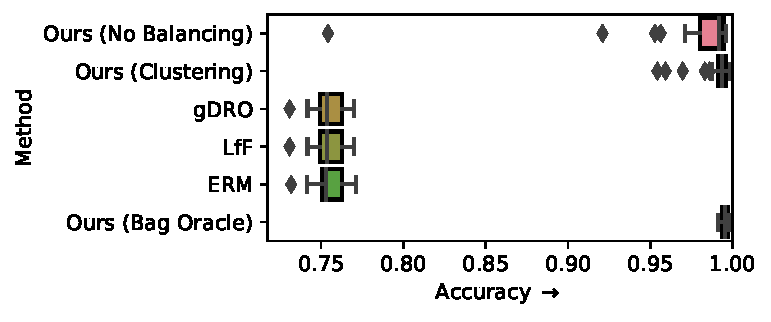
\includegraphics[width=0.49\textwidth]{supmatch/figures/cmnist/subgroup_bias/cmnist_2v4_partial_acc.pdf}
  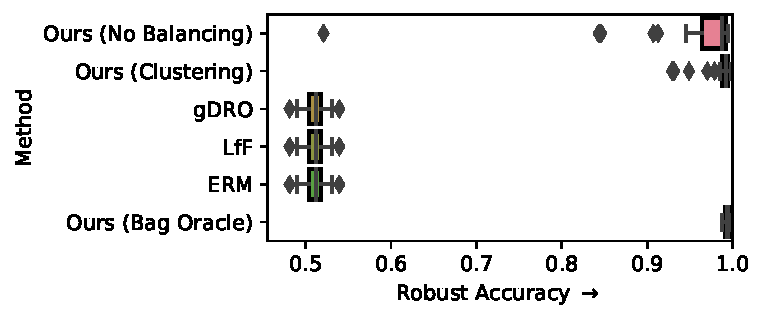
\includegraphics[width=0.49\textwidth]{supmatch/figures/cmnist/subgroup_bias/cmnist_2v4_partial_acc-min.pdf}
%   \includegraphics[width=\columnwidth]{figures/cmnist_2v4_partial_tpr.pdf}
%   \includegraphics[width=\columnwidth]{figures/cmnist_2v4_partial_tnr.pdf}
  \caption{
    Results for the \emph{subgroup-bias} scenario where {\color{purple}purple} fours constitute the missing source.
    %
    The clustering accuracy for \texttt{Ours (No Balancing)} was 96\% $\pm$ 6\%.
    %
    Our method consistently outperforms the baselines, which fare no better than random on the subgroup with the missing source. 
    %
    As we would expect, the median and IQR of our method are positively- and negative- correlated, respectively, with how well the bags of the deployment set are balanced, with \texttt{Ours (Bag Oracle)} providing an upper bound for this.
    %
    Indeed, in one case \texttt{Ours (No Balancing)} failed to outperform the baselines, yet through
    clustering the worst-case \texttt{Robust Accuracy} is limited to within the $95\%$ region.
  }%
  \label{fig:cmnist-2v4-partial}
% \end{figure*}
% \begin{subfigure}
  \end{subfigure}
  
  \begin{subfigure}[b]{\textwidth}
  \centering
  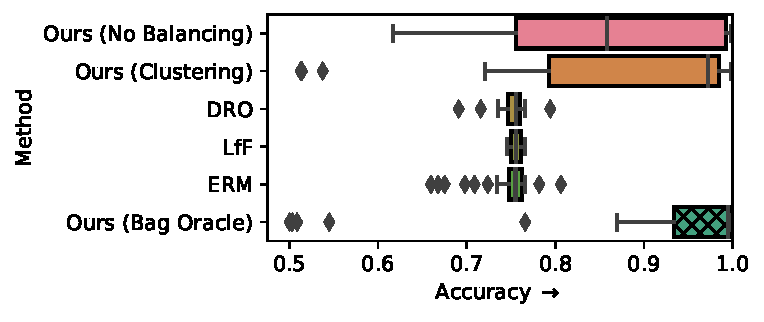
\includegraphics[width=0.49\textwidth]{supmatch/figures/cmnist/missing_subgroup/cmnist_2v4_miss_s_acc.pdf}
  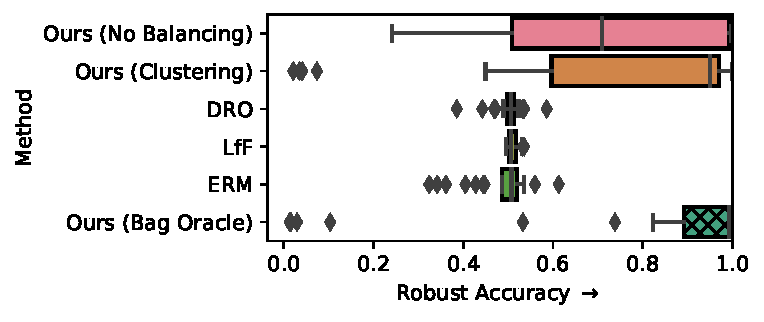
\includegraphics[width=0.49\textwidth]{supmatch/figures/cmnist/missing_subgroup/cmnist_2v4_miss_s_acc-min.pdf}
%   \includegraphics[width=\columnwidth]{supmatch/figures/cmnist_2v4_miss_s_alt_tpr.pdf}
%   \includegraphics[width=\columnwidth]{supmatch/figures/cmnist_2v4_miss_s_alt_tnr.pdf}
  \caption{
    Results for the \emph{missing-subgroup scenario} where {\color{purple}purple} digits constitute the missing subgroup.
    %
    The clustering accuracy for \texttt{Our (No Balancing)} was 88\% $\pm$ 5\%. 
    This scenario is significantly more difficult to solve than the subgroup-bias as there is insufficient inductive bias in the labels and the deployment set for the support matching to be well-posed. 
    %
    This is reflected in the high variance of our method, variance, however, which can be drastically reduced by improving the quality of balancing.
    %
    Nevertheless, all variants of our method perform significantly better than the baselines in terms of the median \texttt{Robust Accuracy}, and the rate at which they produce degenerate solutions (marked by performance worse than \texttt{ERM}'s) relatively low.
    %
  }%
  \label{fig:cmnist-2v4-miss-s}
  \end{subfigure}
  \caption{
  Results for two-digit Colored MNIST for two different scenarios (subgroup bias (Top) and missing subgroup (Bottom)) in the form of box plots of the \texttt{Robust Accuracy} (the minimum accuracy computed over the subgroups) over \textbf{30 repeats}.
  }
\end{figure*}

%
Appendix~\ref{sec:dataset-construction} provides description of the dataset and the settings used
for \( D^{dep} \) and \( D^{tr} \). 
%
Each source is then a combination of digit-class (class label) and colour (subgroup label). 
%
We begin by considering a binary, 2-digit/2-colour, variant of the dataset with $\gY = \{2, 4\}$
and $\gS = \{\text{\color{green}green}, \text{\color{purple}purple}\}$.
(Appendix~\ref{ssec:3-digit-3-color} provides results for 3-digit/3-colour variant.) 
%
For this variant we explore both the SB (subgroup bias) setting and a more extreme \emph{missing
subgroup} setting.
%
To simulate the SB setting, we set \(\gS^{tr}_{ Y=4 }=\{\text{\color{green}{green}}\}\). 
%
In the \emph{missing subgroup} setting, $S=\text{\color{purple}{purple}}$ is missing from
\(\gS^{tr}_{ Y=2 }\) as well, so that all classes only have support in
\(\{\text{\color{green}{green}}\}\).
%
However, for this scenario, the disentangling procedure has more than one possible solution --
apart from the natural solution, it is also possible to consider ($Y=2$,
$S=\text{\color{green}{green}}$) and ($Y=4$, $S=\text{\color{purple}{purple}}$) as forming one
factor in the disentangling, with the other factor comprising the two remaining
$s$-$y$-combinations.
%
Such an ``unnatural'' disentangling (spanning digit class \emph{and} colour) is avoided only by the
tendency of neural networks to prefer simpler solutions (Occam's razor) and in general we cannot
guarantee that this pathological case be avoided based only on the information provided by the
training labels and deployment set.

To establish the effectiveness of our method, we compare against four baselines.
%
The first is \texttt{ERM}, a classifier trained with cross-entropy loss on this data; the second is
\texttt{DRO} \citep{HasSriNamLia18}, which functions without subgroup labels by minimising the
worst-case training loss over all possible groups that are above a certain minimum size; the third
is \texttt{gDRO} \citep{sagawa2019distributionally}, which minimises the worst-case training loss
over predefined subgroups but is only applicable when $|\gS^{tr}| > 1$; the fourth is \texttt{LfF}
\citep{NamChaAhnLeeetal20} which reweights the cross-entropy loss using the predictions of a
purposely-biased sister network.
%
For fair comparison, the training set is balanced according to the rules defined in
\S\ref{sec:sm-adversarialsm} for all baselines.

Fig.~\ref{fig:cmnist-2v4-partial} shows the results for the SB setting. 
%
We see that the performance of our method directly correlates with how balanced the bags are, with
the ranking of the different balancing methods being \texttt{Oracle} $>$ \texttt{Clustering}$>$
\texttt{No Balancing}. 
%
Even without balancing, our method greatly outperforms the baselines, which all perform similarly.

Fig.~\ref{fig:cmnist-2v4-miss-s} shows that the problem of \emph{missing subgroups} is harder to
solve.
%
For all balancing strategies, the IQR is significantly higher than observed in the SB setting, with
the latter also giving rise to a large number of extreme outliers. 
%
The median, however, remains high, indicative of a ``hit-or-miss'' aspect to the method, albeit
with the number of hits far outweighing the misses. 
%
Visualisations of the reconstructions (Appendix~\ref{sec:qual-results})
suggest that the extreme outliers correspond to the degenerate solution mentioned above.
% with $z$ zeroed-out suggests that misses often mostly occurred due to the semantic information
% being concentrated in $\tilde{s}$ while $z$ is left to contain only residual information, even
% when $\tilde{s}$ was set to be one-dimensional and binarized. 
%
% We leave it to future work to explore how to better obviate such degeneracies.

% \begin{figure}[tbp]
%   \centering
%    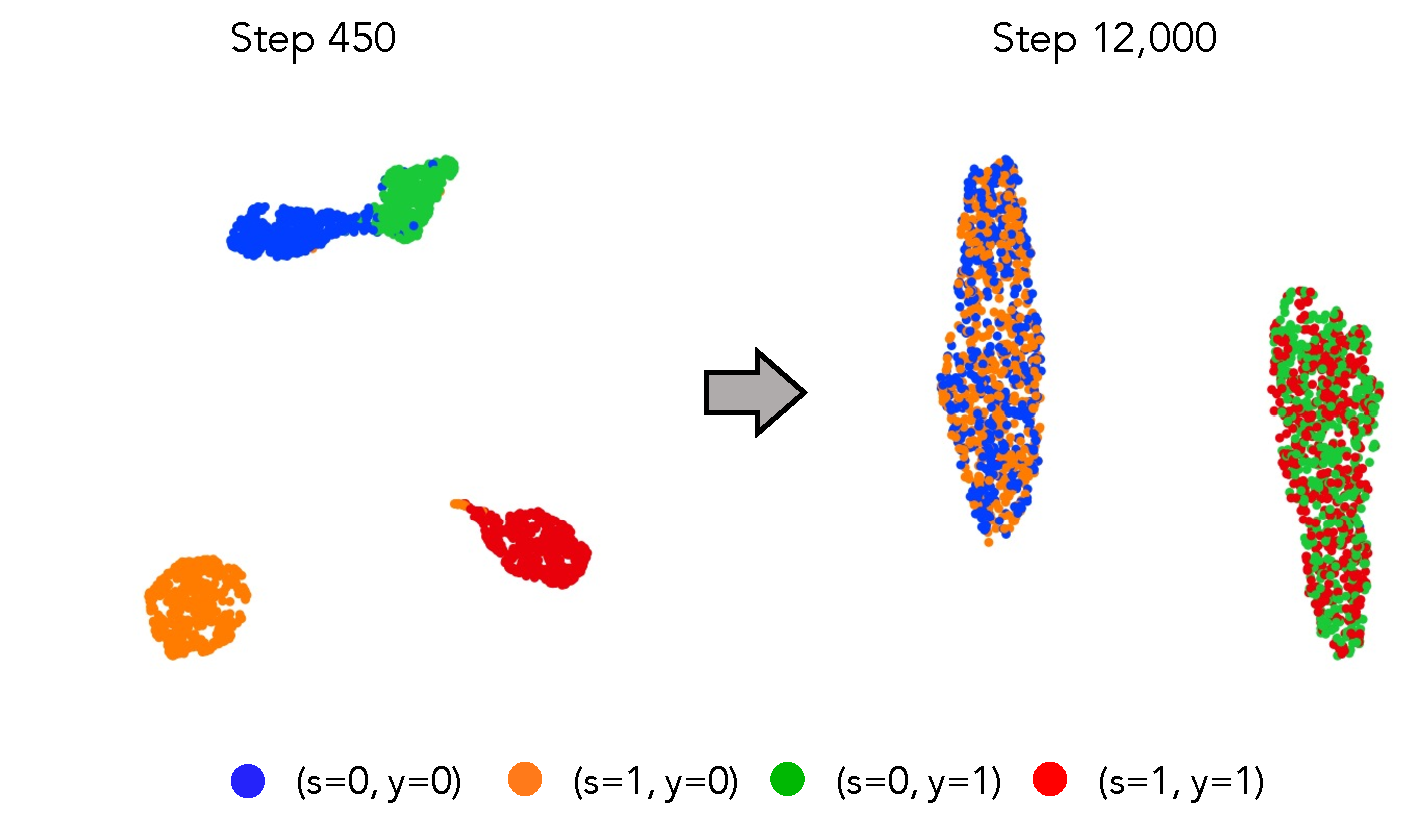
\includegraphics[width=0.6\columnwidth]{supmatch/figures/illustrations/umap_viz.pdf}
%   \caption{%
%     UMAP visualisations of the representations learned by the debiaser for the Colored MNIST
%     dataset. \textbf{Left}: After 450 training-steps each source forms a distinct cluster.
%     \textbf{Right}: After 12,000 training-steps sources with the same $y$-value have merged, thus
%     eliminating the spurious correlation between digit and color.
%   }%
%   \label{fig:umap}
% \end{figure}

% We visualise the learned representation -- from a successful run -- using UMAP
% \citep{mcinnes2018umap} in Fig.~\ref{fig:umap}. % Here, we see that at the beginning of training,
% all four sources are distinct, and the two sources with $s=0$ (from which one is missing in the
% training set) are closer to each other than to their respective classes. % At the end of
% training, the representations clearly separate into two clusters corresponding to the two
% classes, while the subgroups are distributed evenly therein.

\subsection{CelebA}\label{ssec:celeba_exp}
%
\begin{figure*}[t]
  \centering
  % Smiling females missing
%   \normalsize{Missing source: smiling females}\par\medskip
%  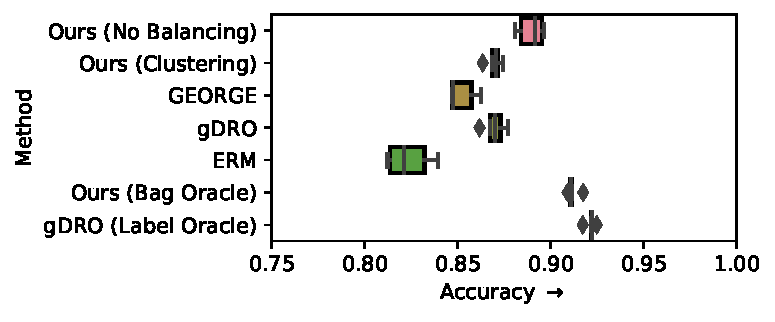
\includegraphics[width=0.49\textwidth, height=3cm]{supmatch/figures/celeba/no_smiling_females/celeba_gender_smiling_acc.pdf}
 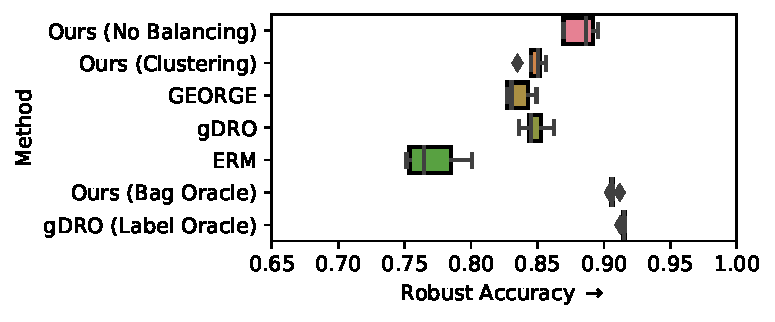
\includegraphics[width=0.49\textwidth]{supmatch/figures/celeba/no_smiling_females/celeba_gender_smiling_acc-min.pdf}
    % Smiling males missing
%   \normalsize{Missing source: smiling males}\par\medskip
%  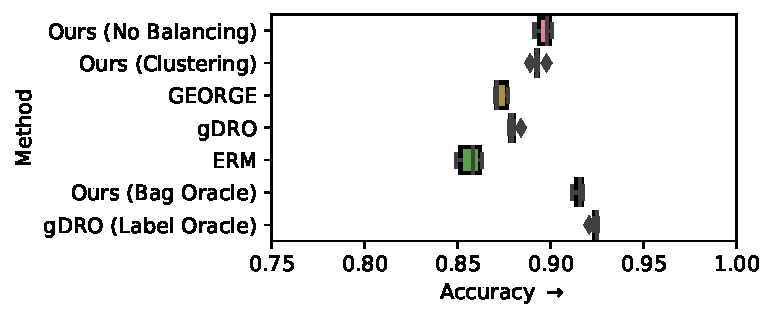
\includegraphics[width=0.49\textwidth]{supmatch/figures/celeba/no_smiling_males/celeba_gender_smiling_acc.pdf}
 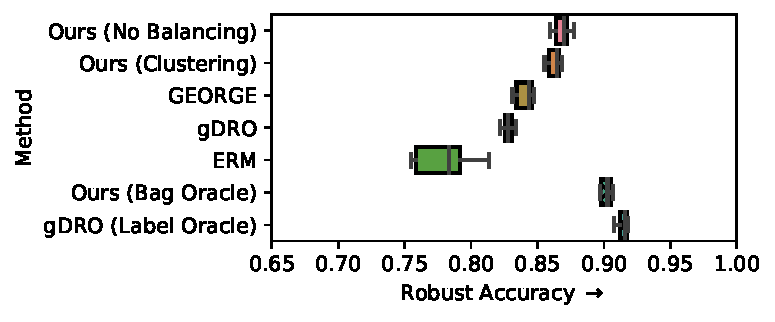
\includegraphics[width=0.49\textwidth]{supmatch/figures/celeba/no_smiling_males/celeba_gender_smiling_acc-min.pdf}
    % Unsmiling females missing
%   \normalsize{Missing source: non-smiling} females\par\medskip
%  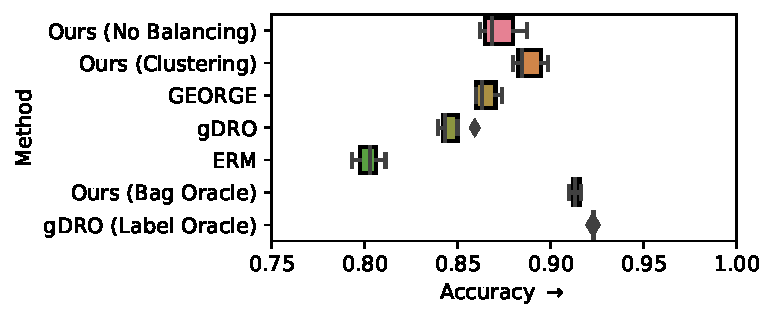
\includegraphics[width=0.49\textwidth]{supmatch/figures/celeba/no_unsmiling_females/celeba_gender_smiling_acc.pdf}
 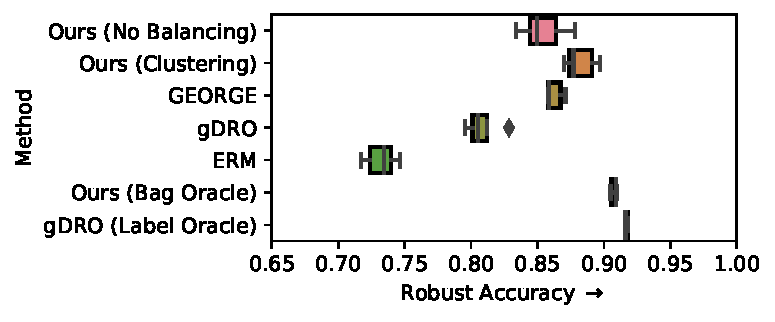
\includegraphics[width=0.49\textwidth]{supmatch/figures/celeba/no_unsmiling_females/celeba_gender_smiling_acc-min.pdf}
  % Unsmiling males missing
%   \normalsize{Missing source: non-smiling males}\par\medskip
%  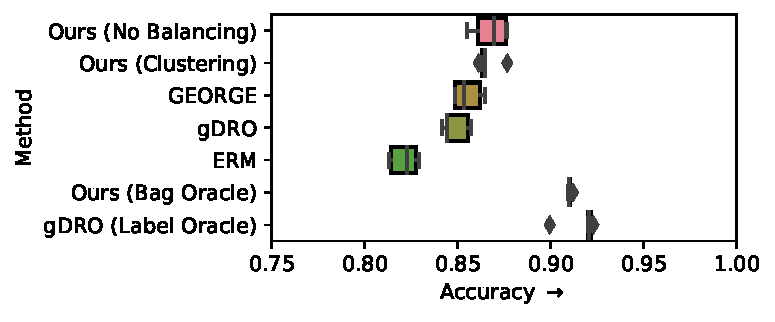
\includegraphics[width=0.49\textwidth]{supmatch/figures/celeba/no_unsmiling_males/celeba_gender_smiling_acc.pdf}
 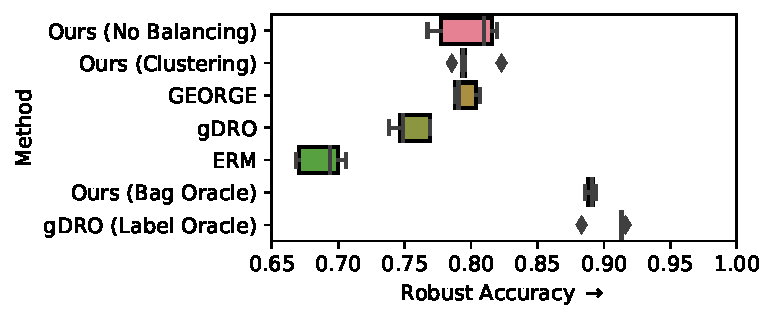
\includegraphics[width=0.49\textwidth]{supmatch/figures/celeba/no_unsmiling_males/celeba_gender_smiling_acc-min.pdf}

% compressed figures:
%   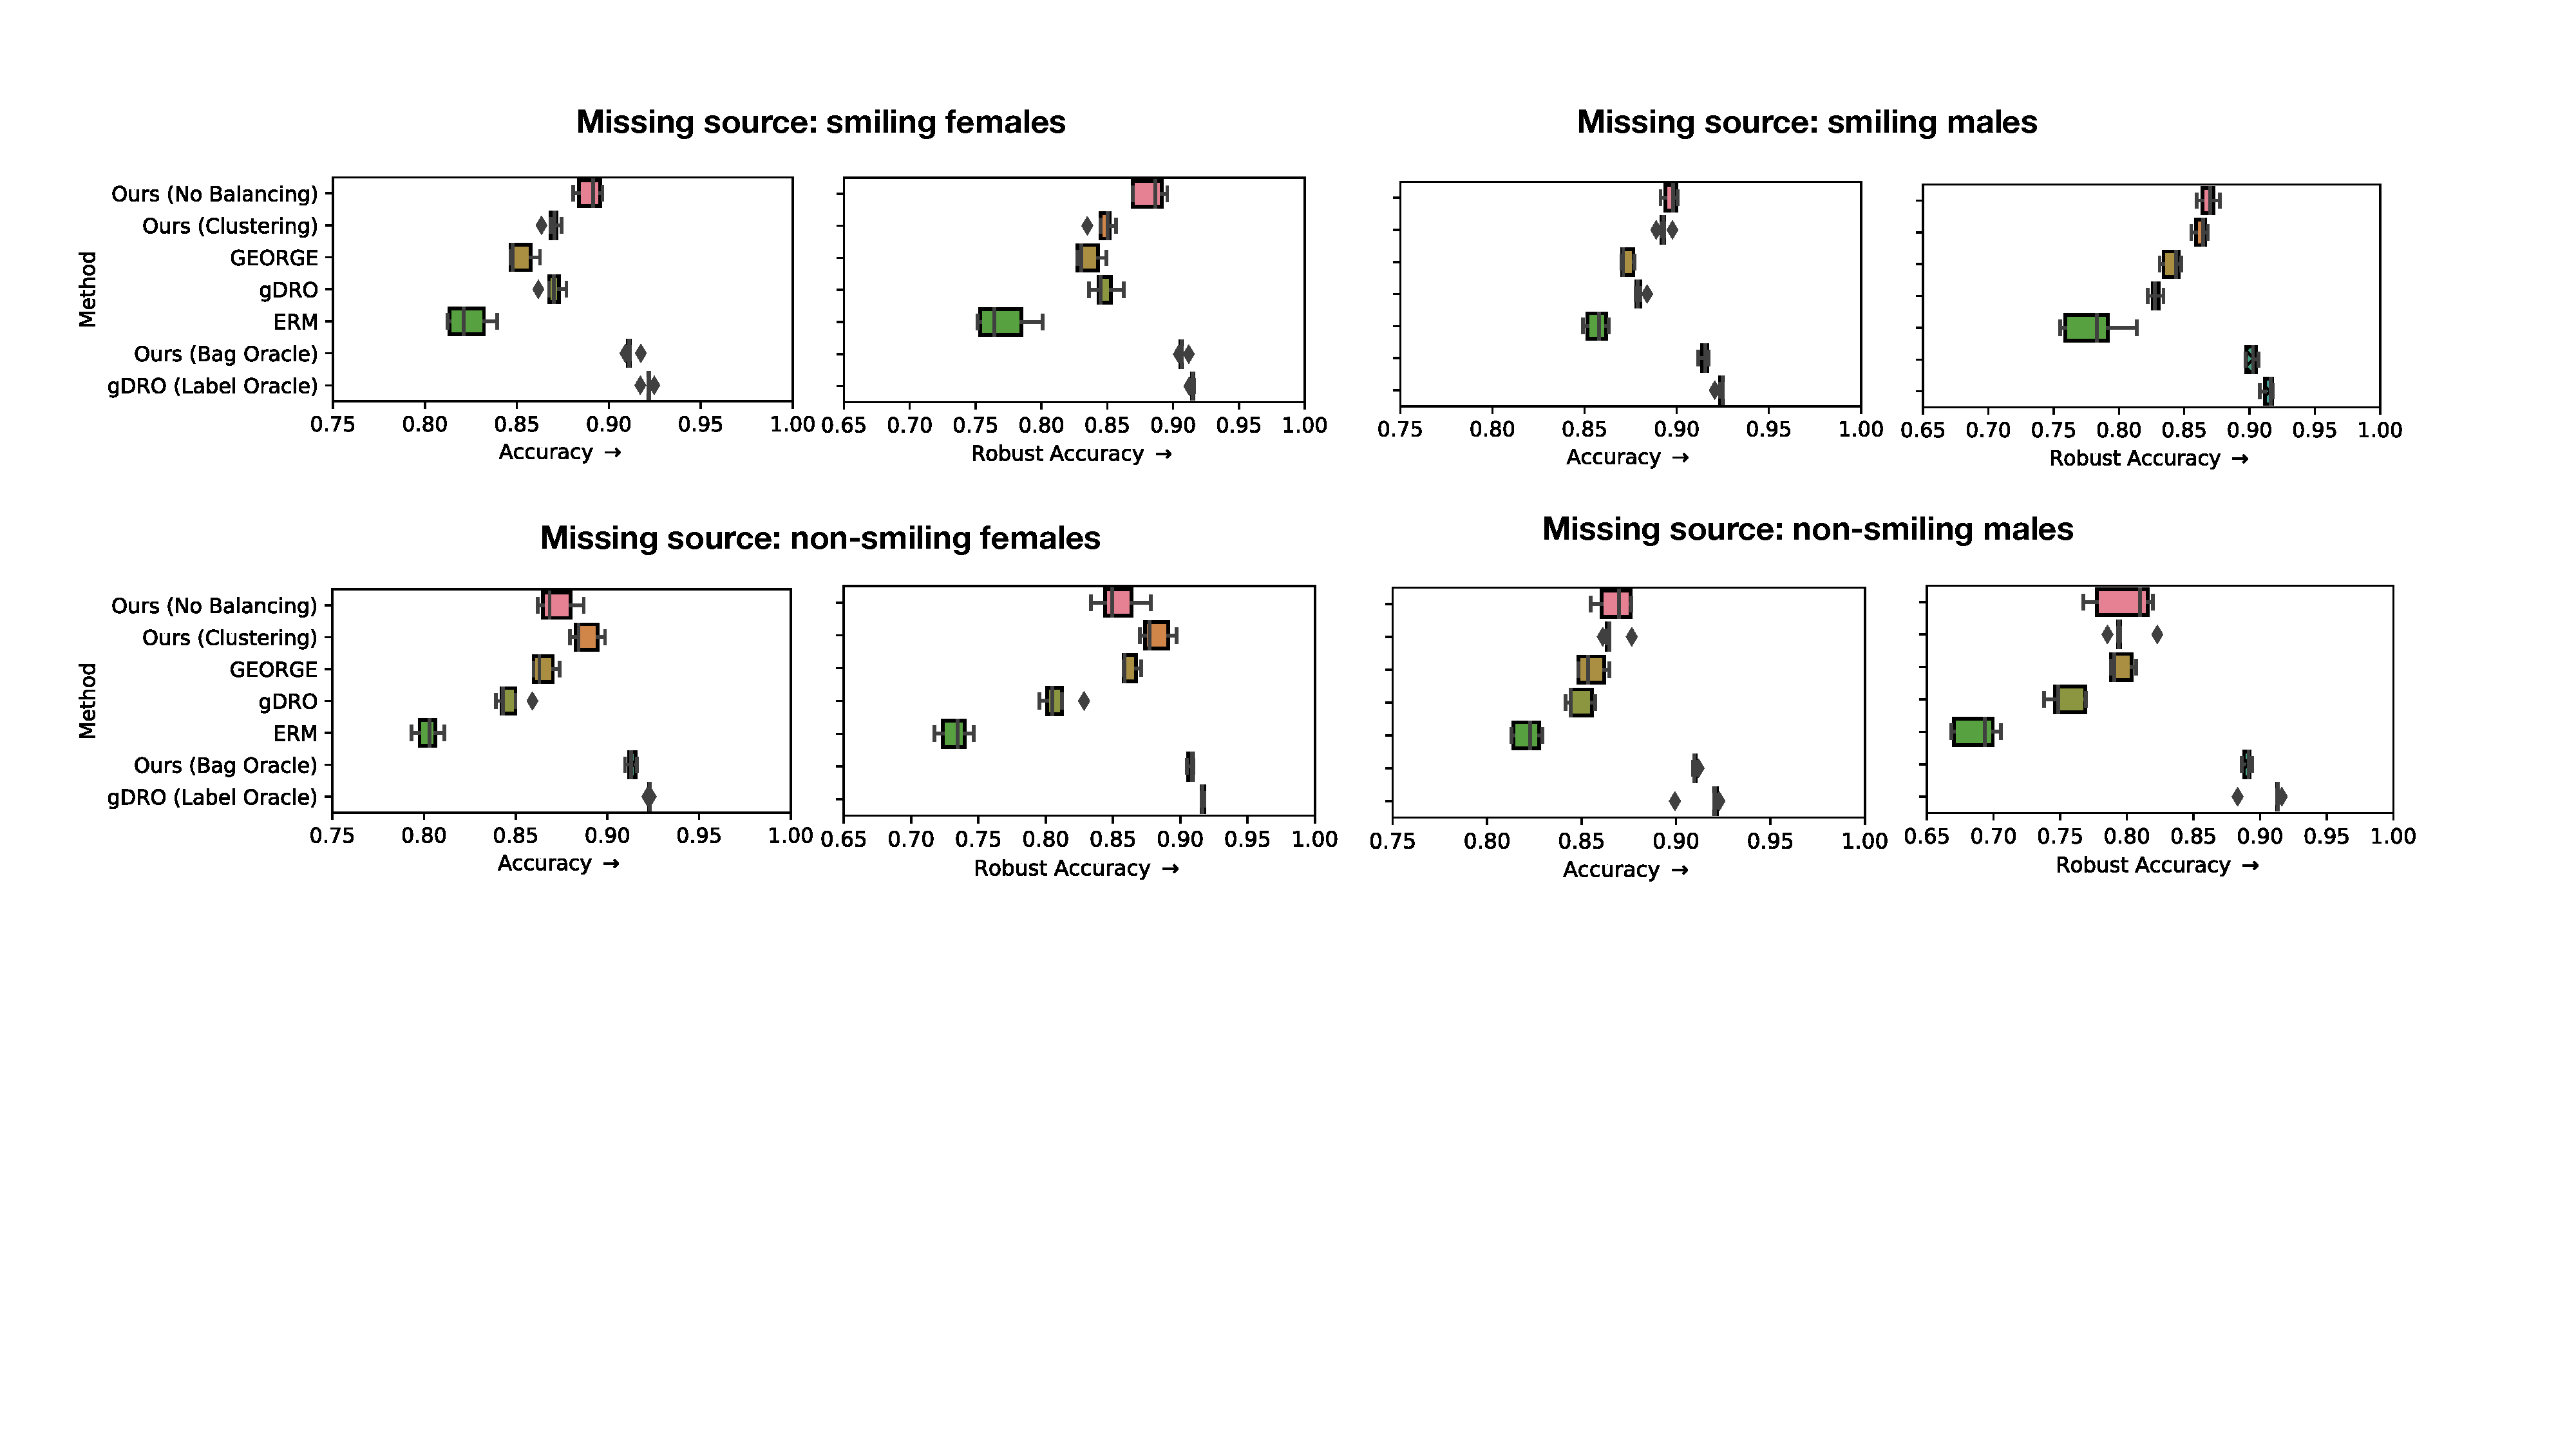
\includegraphics[width=1.0\textwidth]{supmatch/figures/celeba/CelebA2.pdf}
  \caption{
    Results from \textbf{5 repeats} for the CelebA dataset for the \emph{subgroup bias} scenario.
    The task is to predict ``smiling'' vs ``non-smiling'' and the subgroups are based on gender. 
    %
    The four sources are dropped one at a time from the training set
    (\textbf{Top Left}: smiling females; \textbf{Top Right}: smiling males; \textbf{Bottom Left}: non-smiling females;
    \textbf{Bottom Right}: non-smiling males), while the deployment set is kept fixed.
    %
    \texttt{Robust Accuracy} refers to the minimum accuracy computed over the subgroups.
    %
    Our method consistently performs on par with or outperforms \texttt{GEORGE} (which in turn outperforms \texttt{ERM}).
    %
    We note that in some of the runs, \texttt{GEORGE} performed no better than random -- these results were truncated for visibility but can be found in
    Fig.~\ref{fig:celeba-gender-smiling-full}.
    %
    % Due to poor clustering accuracy and the fact that the deployment set is naturally relatively well-balanced with respect to gender, \texttt{Ours (Clustering)} failed to improve on \texttt{Ours (No Balancing)} for all but one missing source.
    %
    Given \emph{indirect} supervision from the deployment set in the form of oracle-balancing, our method performs similarly to \texttt{gDro (Label Oracle)} that receives \emph{direct} supervision.
  }%
  \label{fig:celeba-gender-smiling}
\end{figure*}


%
To demonstrate our method generalises to real-world computer vision problems, we consider the
CelebA dataset~\citep{liu2015celeba} comprising over 200,000 images of different celebrities. The
dataset comes with per-image annotations of physical and affective attributes such as `Smiling',
`Gender', hair colour, and `Age'.
%
Since the dataset exhibits natural imbalance with respect to $\gG$, we perform no additional
sub-sampling of either the training set or the deployment set. We predict ``smiling'' as the class
label and use the binary attribute, ``gender'', as the subgroup label. Here, we consider the SB
setting but rather than just designating one missing source, we repeat our experiments with each
source being dropped in turn.
%
As before, we evaluate our method under three balancing schemes and compare with ERM and gDRO
trained on only the labelled training data.
%
We also compare with two other variants of gDRO: 1) \texttt{gDRO (Label Oracle)}, a variant that is
trained with access to the ground-truth labels of the deployment set, thus providing an upper-bound
on the downstream classification performance; 2) \texttt{GEORGE} \citep{SohDunAngGuetal20}, which
follows a two-step procedure of first clustering to obtain the labels for hidden subgroups, and
then using these labels to train a robust classifier using gDRO.
%
\citet{SohDunAngGuetal20} consider a different version of the problem (termed
\emph{hidden-stratification}) in which the class labels are known for all samples but the
subgroup-labels are missing entirely.
%
We adapt \texttt{GEORGE} to our setting by modifying the semi-supervised clustering algorithm to
predict the marginal distributions (\(P(Y|X)\) and \(P(S|X)\) instead of the joint distribution
\(P(Y, S|X)\), allowing us to propagate the class labels from \( D^{tr} \) to \( D^{dep} \) (see
Appendix~\ref{adapting_g} for details).
% Following this, gDRO is trained on the combination of the training and deployment sets, with the
% latter's labels conferred by clustering.


Fig.~\ref{fig:celeba-gender-smiling} shows the results for experiments for each missing source,
showing similar trends across all instantiations of the SB scenario. 
%
\texttt{gDRO (Label Oracle)} consistently achieves the best performance according to both metrics,
with \texttt{Our Method (Bag Oracle)} consistently coming in second. 
%
We note that while both methods use some kind of oracle, the \emph{label oracle} provides
\emph{all} class/subgroup labels to its algorithm, whereas the \emph{bag oracle} only balances the
bags. 
%
Despite the large difference in the level of supervision, the margin between the two oracle methods
is slim. 
%
We observe that clustering in many cases impairs performance which can be explained by poor
clustering of the missing source ($\sim$60\% accuracy).
%
CelebA exhibits a natural imbalance with respect to gender/smiling but not a significant one,
allowing for random sampling to yield a reasonable approximation to the desired perfect bags. 
%
We believe adjustments to the clustering algorithm -- e.g.\ using a self-supervised loss instead of
a reconstruction loss for the encoder -- could close the gap between clustering-based and
oracle-based balancing. 
%
Nonetheless, among the non-oracle methods, variants of our method
consistently match or exceed the performance of the baselines. 
%
While the plots show \texttt{GEORGE} can perform strongly in this SB scenario, we note that for
several of the missing sources, the method failed catastrophically in one out of the five runs.
%
We have cut off those data points here so as not to compromise the visibility of the other results;
the full versions of the plots can be found in Appendix~\ref{ssec:extended-results-celeba}.
%
The fact that \texttt{GEORGE} leverages both the training and deployment sets in a semi-supervised
way with clustering makes it the baseline most comparable to our method.
%
However, its performance is much more dependent on the clustering step than our method.

% %
% \subsection{Chest-Xray8}{\label{ssec:nih_exp}}
% %
% The Chest-Xray8 dataset \citep{wang2017chestx}  comprises 108,948 frontal-view X-ray images with
% weak labels -- mined automatically from radiology reports using natural language processing --
% indicating positive diagnosis of eight thoracic diseases. 
% %
% These labels are mutually inclusive and as such give rise to a multi-label classification task. 
% %
% Among the images, 24,636 are associated with one or more pathologies, while the remaining 84,312
% are derived from healthy patients.
% % Atelectasis, Cardiomegaly, Effusion, Infiltration, Mass, Nodules, Pneumonia, Pneumothorax
% To simplify the analysis, we convert the problem into one of binary classification by considering
% only he most frequently occurring pathology, ``infiltration''. 
% %
% We note that, since our method only uses the target implicitly via balancing in order to learn
% invariance to the subgroup, and this objective is balanced with the goal of maximally preserving
% information about the input, \( \gI(f(X);X) \), rather than the target directly, the resulting
% representation could be can be used for any of the targets without detriment. 
% %
% We designate ``gender'' as the subgroup label, following \citep{seyyed2020chexclusion}, and
% simulate the SB setting by dropping from the training set male patients with a positive diagnosis,
% i.e. by setting \(\gS^{tr}_{ Y=\text{infiltration} }=\{\text{female}\}\).


% \subsection{Sensitivity Analysis}\label{ssec:sensitivity}

% To assess the empirical robustness of our algorithm to noise in the bag-balancing, we conduct an
% sensitivity analysis using the Chest-Xray8 dataset. 
% %
% Using the same configuration used to collect the results from the previous section, we run our
% algorithm with the ground-truth labels used for balancing but with \( \{5\%, 10\%, \dots, 50\%\} \)
% of the labels perturbed (flipped). 
% %
% Rather than randomly perturbing the labels by sampling from the set of complementary labels --
% i.e., \( \tilde{g}_i \sim \mathrm{uniform}(\gG \setminus \{g_i\}) \), with \( g_i \) and \(
% \tilde{g}_i \) denoting the ground-truth and the perturbed labels, respectively -- which yields
% unrealistic perturbations due to the discounting the semantic relationships between groups
% (semantically similar groups are more likely to be confused by a clustering algorithm) we instead
% sample a perturbed label, $\tilde{g}_i$ from $\gG$ with probability proportional to the similarity
% between the associated (featurised) sample and the \(\tilde{g}_i\)th centroid, \(
% \phi_{\tilde{g}_i} \in \mathbb{R}^d \), with the constraint that the perturbed label does not equal
% the original one. 
% %
% This is done using features extracted by a pre-trained CLIP \citep{radford2021learning} visual
% encoder. Namely, the centroids \( \Phi \in \mathbb{R}^{|\gG| \times d} \) are computed as the
% group-conditional means of these features, over the deployment set, and their similarity with a
% given sample's features is measured using cosine similarity. 
% %
% Assuming \(L_2\)-normalised CLIP features, $\bar z_i^\text{CLIP} \in \mathbb{R}^d$, and prototypes,
% $\bar \Phi$, the sampling scheme used to generate the perturbed label, $\tilde{g}_i$, for a given
% ground-truth label, $g_i$, can be written as
% %
% \begin{align}
%   %
%   \tilde{g}_i \sim \text{Cat}(\gG, \bigtriangleup_\mathbf{w} ), \quad
%   %
%   \bigtriangleup_\mathbf{w} \triangleq  \frac{\mathbf{w}}{\sum_j \mathbf{w}_j} , \quad
%   %
%   \mathbf{w} \triangleq \text{exp}(\bar z_i^\text{CLIP} \cdot \bar \Phi \tau^{-1})
%   \odot (1 - e_{g_i}),
%   %
% \end{align}
% %
% where \( \text{Cat} \) denotes the categorical distribution with support \(\gG\) and sampling
% probabilities \( \bigtriangleup_w \), \( \tau \in \mathbb{R}^+_\ast \) denotes a temperature
% parameter modulating the sharpness of the sampling distribution, \(e_{g_i}\) denotes the one-hot
% encoding of \(g_i\), and \(\odot\) denotes the Hadamard product that is used with \(e_{g_i}\) to
% mask out the \(g_i\)th prototype and thereby enforce \( \tilde{g}_i \neq g_i \).

% which shows strong performance even without balancing.

% Now that we have them, we can discuss the results with clustering.
%
% We did not use the clustering approach for CelebA, as the attributes ``smiling'' and ``gender''
% are not the most salient; more work is needed on the clustering side to discover all semantically
% meaningful clusters.
%
% Nonetheless, our method consistently outperforms the baselines even when no balancing is applied
% Furthermore, we show qualitative results of the disentangling in fig.~\ref{fig:celeba-recons},
% and note a clear separation of subgroup-relevant information from subgroup-irrelevant
% information.
%in $g(0, f_s(x))$ and $g(f(x), 0)$, respectively.

%Furthermore, we control the \emph{number of clusters},which means all samples can get sorted into
%the right \emph{number of groups}. 
%
% Instead we use the idea of balanced dataset and sample equal amount of samples from each cluster
% to form a batch. 
  
% \textbf{Disentangled representations via adversarial autoencoders}
%We want to learn a disentanglement using a perfect dataset as the supervision signal.
%
%To achieve this, our semi-supervised disentanglement learning framework (fig.
%\ref{fig:architecture} ) maps data points into independent factors of variations such that our
%training dataset $D_{\text{tr}}$ and our deployment set $D_c$ are indistinguishable; i.e., we
%would like transform $D_{\text{tr}}$ such that the independence condition $y\perp s$ holds.
%
%However, the deployment set itself $D_c$ might not amount to a suitable target distribution in
%which the independence condition holds.
%
%The idea is to make the deployment set $D_c$ approximately perfect by balancing it according to
%the cluster IDs, forming the set $D_p$.
%
% We create disentangled representations by training four separate neural networks, which we denote
% $f$, $g$, $h$ and $l$. % We use mean squared error for the reconstruction loss, and the binary
% cross entropy error for the discriminator loss. % For a dataset with mixed-typed attributes, we
% use a combination of mean squared error and (binary) cross entropy error for the reconstruction
% loss. % We optimize the proposed model using a scheduled update scheme where we freeze the
% weights of the autoencoder and predictor modules when we update the weights of the discriminator,
% and vice versa.
%



\section{Related work}
\label{sec:related-work}
\paragraph{Invariant learning}
\citet{SohDunAngGuetal20} and \citet{creager2021environment} both consider a similar problem, where
the data also exhibits a two-level hierarchy formed by classes and subgroups.
%
In contrast to our work, however, there is no additional bias in the data; while they may be
unobserved, the labelled data is assumed to have complete class-conditional support over the
subgroups.
%
As such, these methods are not directly applicable to the particular form of the problem we
consider.
%
Like us, \citet{SohDunAngGuetal20} uses semi-supervised clustering to uncover the hidden subgroups,
however their particular clustering method requires access to the class labels not afforded by the
deployment set, as does the training of the robust classifier.

\paragraph{Unsupervised domain adaptation}
In unsupervised domain adaptation (UDA), there are typically one or more source domains, for which
training labels are available, and one or more unlabelled target domains to which we hope to
generalise the classifier.
%
A popular approach for solving this problem is to learn a representation that is invariant to the
domain using adversarial networks \citep{ganin2016domain} or non-parametric discrepancy measures
such as MMD \citep{gretton2012kernel}.
%

There are two ways in which one can compare UDA to our setting: 1) by treating the subgroups as
domains; and 2) by treating the training and the deployment set as ``source'' and ``target''
domains, respectively.
%
The first comparison is exploited in algorithm fairness, yet does not carry over to our setting in
which the labelled data contains \emph{incomplete} domains. 
%
When all sources from a given domain are missing then there are no domains to be matched, and even
when this is not the case, matching will result in misalignment due to differences in
class-conditional support.
%
The second comparison is more germane but ignores an important aspect of our problem: the presence
of spurious correlations.
%

Similar to us, \citet{tong2022adversarial} utilise adversarial methods to align the support of two
distributions in a semi-supervised regime -- specifically, they propose to use symmetric support
difference as a divergence measure which they realise using a discriminator. 
However, their method focuses on label-shift in the UDA
setting and does not consider the hierarchical structure that exists within the source (training)
and target (deployment) domains, and as such they do not consider the notion of ``missing sources''
that can arise due to said structure -- the characterisation of this problem is one of the two
main contributions of this work (the other being our proposed solution). Furthermore, the
discriminator used therein is applied instance-wise; we show in \ref{sec:ablations} that allowing
the discriminator to model inter-sample relationships has tangible addition benefits when
performing support-matching.

\paragraph{Multiple instance learning}
Multiple instance learning \citep{maron1998framework} is a form of weakly-supervised learning in
which samples are not labelled individually part as part of a set or \emph{bag} of samples.
%
In the simplest (binary) case, a bag is labelled as positive if there is a single instance of a
positive class contained within it, and negative otherwise.
%
In our case, we can view the missing sources as constituting the positive classes, which leads to
all bags (a term we will use throughout the paper distinctly from ``batches'') from the deployment
set being labelled as positive, and all bags from the training set being labelled as negative.
%
Given this labelling scheme, we make use of an adversarial set-classifier to align the supports of
the training and deployment sets in the representation space of an encoder network.
%

\paragraph{Positive unlabelled learning}
Learning from positive and unlabelled data, or \emph{PU learning}, refers to the
binary-classification setup in which the labelled training data consists of only positive samples
while additional unlabelled data is assumed to contain both positive and negative samples
\citep{liu2002partially, liu2003building, bekker2020learning}. This is analogous to our problem
setting if we consider the positive class to be all samples sources represented in the training
set, collectively, while the missing sources collectively make up the negative class. However, the
goal here is not merely to learn the classification boundary between the present and missing
sources but to learn to classify the target class of a given sample independently of its subgroup.
This is equivalent to requiring that a classifier trained to distinguish between positive and
negative classes, according to the aforementioned PU learning setup, from the pre-logits layer of
our desired classifier be maximally entropic -- we propose to use adversarial learning to achieve
this.

% \paragraph{Fairness}


\section{Conclusion}
\label{sec:conclusion}
%
\corr{
  %
In this paper, we formalised the problem that systematic bias or dataset curation resulting in one or more
subgroups having zero labelled data; we hope our doing so stimulates serious consideration
for it in the planning, building, and evaluating systems.
%
This complements concurrent research by \citet{yang2023change} wherein the same problem (with
different formalism) is alluded to, but its solution left as an open question.
%
Contrastingly, we proposed here a two-step approach for addressing the problem within a
semi-supervised framework. 
%
The first step entails constructing hierarchically-balanced bags from an unlabelled deployment set
via one's semi-supervised clustering algorithm of choice.
%
The second step then entails matching the support, instead of the raw distributions, of the
training and deployment sets in representation space, so as to learn subgroup-invariant
representations, an outcome we prove corresponds to the optimum of the proposed objective function.
%
We empirically validate our frame\-work on the Coloured MNIST and CelebA datasets, showing it
possible to maintain high performance on subgroups with incomplete support.
%
Furthermore, we bound the error in the objective incurred due to imperfect clustering and show that
the proposed set-wise discriminator is empirically more robust to this error than conventional
instance-wise discriminators.
%
Future work includes the exploration of other \ac{UL} methods for realising the \ac{MI} component
of the objective and addressing the limitations raised in \S\ref{sec:sm-limitations}.

\subsection{Dataset representativity}
%
The results presented in this version of the paper are for toy (Coloured MNIST) or pseudo-toy
(CelebA) datasets; though both datasets have featured extensively in the literature on
distributional-robust learning (\citealp{arjovsky2019invariant, kim2019learning,
sagawa2019distributionally, creager2021environment}, inter alia) it is natural to doubt the
representativeness of results on them in relation to real-world problems.  
%
To shore up this shortcoming, we have since conducted experiments with two datasets more emblematic
of real-world realisations of the proposed problem, namely Chest-Xray8 \citep{wang2017chestx} and NICO++
\citep{zhang2023nico++}.
%
The former dataset is appealing as it coincides with the motivating example proffered in
\S\ref{sec:sm-intro}; the latter is so as its class-subgroup structure allows for demonstration in
a non-binary (\wrt{} both marginals) setting, whereas the results contained herein were
preponderantly binary out of both simplicity and convention.
%

\subsection{Sensitivity analysis \wrt{} bag-balancing}
%
As noted, we provided bounds on the error in alignment propagated by the error in
approximating \( \gD^{dep}\) but empirical analysis of the reification of this is lacking. 
%
Accordingly, we have sought to effect this via controlled sensitivity analyses \wrt{} the
balancing.
To achieve this, we run our support-matching algorithm with ground-truth labels used for balancing
but with different proportions (typically \( \{5\%, 10\%, \dots, 50\%\} \)) of said labels
perturbed (flipped or randomly shifted cyclically). 
%
Rather than randomly (uniformly) perturbing the labels by sampling from the set of complementary
labels -- i.e., \( \tilde{g}_i \sim \mathrm{uniform}(\gG \setminus \{g_i\}) \), with \( g_i \) and
\( \tilde{g}_i \) denoting the ground-truth and the perturbed labels, respectively -- which yields
unrealistic perturbations due to the discounting of semantic relationships between groups
(semantically similar groups are more likely to be confused by a clustering algorithm) we instead
sample a perturbed label, $\tilde{g}_i$ from $\gG$ with probability proportional to the similarity
between the featurisation of the associated sample and the \(\tilde{g}_i\)th centroid, \(
\phi_{\tilde{g}_i} \in \mathbb{R}^d \), with the constraint that the perturbed label does not equal
the original one. 

%
The featurisation is performed using a pre-trained (via contrastive captioning) CLIP
\citep{radford2021learning} visual encoder. 
%
Namely, the centroids \( \Phi \in \mathbb{R}^{|\gG| \times d} \) are computed as the
group-conditional means of these features, over the deployment set, and their similarity with a
given sample's features is measured using cosine similarity. 
%
Assuming \(L_2\)-normalised CLIP features, $\bar z_i^\text{CLIP} \in \mathbb{R}^d$, and prototypes,
$\bar \Phi$, the sampling scheme used to generate the perturbed label, $\tilde{g}_i$, for a given
ground-truth label, $g_i$, can be written as
%
\begin{align}
  %
  \tilde{g}_i \sim \text{Cat}(\gG, \bigtriangleup_\mathbf{w} ), \quad
  %
  \bigtriangleup_\mathbf{w} \triangleq  \frac{\mathbf{w}}{\sum_j \mathbf{w}_j} , \quad
  %
  \mathbf{w} \triangleq \text{exp}(\bar z_i^\text{CLIP} \cdot \bar \Phi \tau^{-1})
  \odot (1 - e_{g_i}),
  %
\end{align}
%
where \( \text{Cat} \) denotes the categorical distribution with support \(\gG\) and sampling
probabilities \( \bigtriangleup_w \), \( \tau \in \mathbb{R}^+_\ast \) denotes a temperature
parameter modulating the sharpness of the sampling distribution, \(e_{g_i}\) denotes the one-hot
encoding of \(g_i\), and \(\odot\) denotes the Hadamard product that is used with \(e_{g_i}\) to
mask out the \(g_i\)th prototype and thereby enforce \( \tilde{g}_i \neq g_i \).
%
% CORRECTED: Include any work that you have done since.
}



\section*{Acknowledgments}
\label{sec:ack}
% This research was supported in part by a European Research Council (ERC) Starting Grant for the project ``Bayesian Models and Algorithms for Fairness and Transparency'',
% funded under the European
% Union's Horizon 2020 Framework Programme
% (grant agreement no. 851538).
% Novi Quadrianto is also supported by the Basque Government
% through the BERC 2018-2021 program and by Spanish Ministry of Sciences, Innovation and Universities:
% BCAM Severo Ochoa accreditation SEV-2017-0718.


\newpage
% \section{Additional experiments}\label{sec:additional-results}
% \subsection{Results for Adult Income}\label{sec:adult-results}
% \begin{figure*}[htp]
%     \centering
%     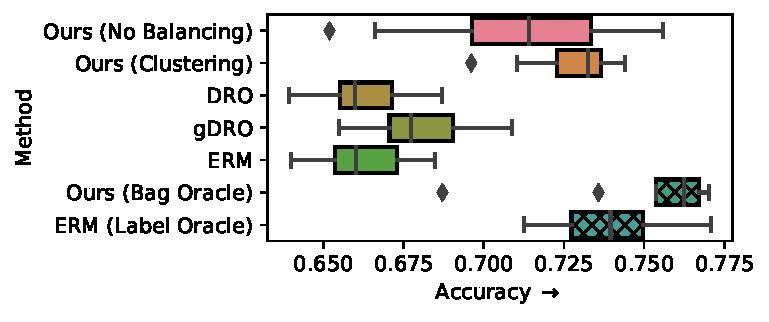
\includegraphics[width=0.49\textwidth]{supmatch/figures/adult/subgroup_bias/adult_partial_acc.pdf}
%     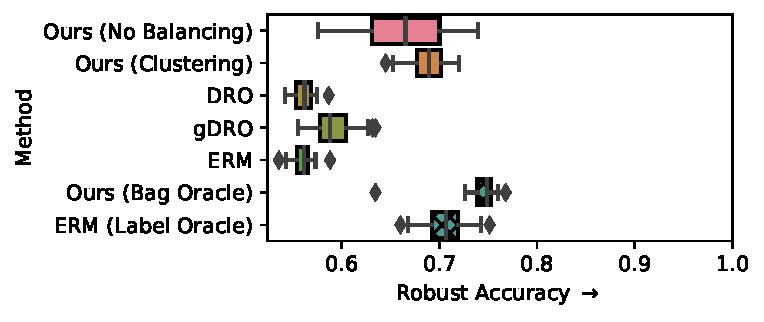
\includegraphics[width=0.49\textwidth]{supmatch/figures/adult/subgroup_bias/adult_partial_acc-min.pdf}
%     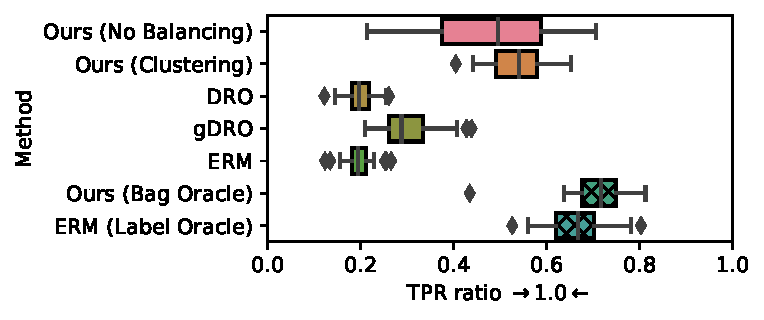
\includegraphics[width=0.49\textwidth]{supmatch/figures/adult/subgroup_bias/adult_partial_tprr.pdf}
%     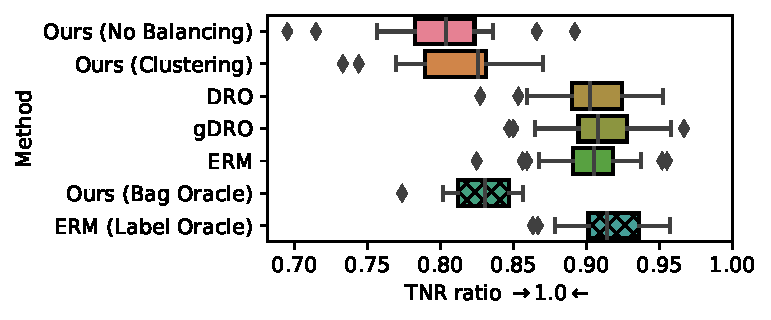
\includegraphics[width=0.49\textwidth]{supmatch/figures/adult/subgroup_bias/adult_partial_tnrr.pdf}
%     \caption{%
%     Results for the Adult Income dataset with \emph{subgroup bias}, for the binary classification
%     task of predicting whether an individual earns $>$\$50,000 with a binary subgrouping based on
%     \emph{gender}. \texttt{ERM (Label Oracle)} refers to a model based on ERM (empirical risk
%     minimization), trained on a labeled deployment set and as such not suffering from bias
%     present in the training set.
%     \textbf{Top left}: Accuracy.
%     \textbf{Top right}: Robust Accuracy.
%     \textbf{Bottom left}: True positive rate ratio.
%     \textbf{Bottom right}: True negative rate ratio.
%     For \texttt{Ours (Clustering)}, the clustering accuracy was 69.7\% $\pm$ 0.3\%;
%     % for \texttt{K-means} it was 43\% $\pm$ 3\%.
%     }%
%     \label{fig:adult-subgroup-bias}
% \end{figure*}
% \begin{figure*}[htp]
%     \centering
%     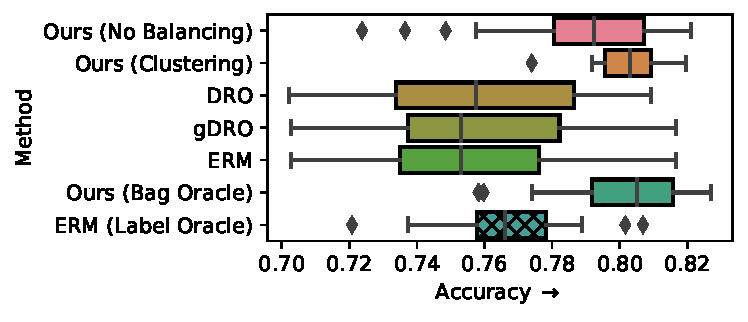
\includegraphics[width=0.49\textwidth]{supmatch/figures/adult/missing_subgroup/adult_miss_s_acc.pdf}
%     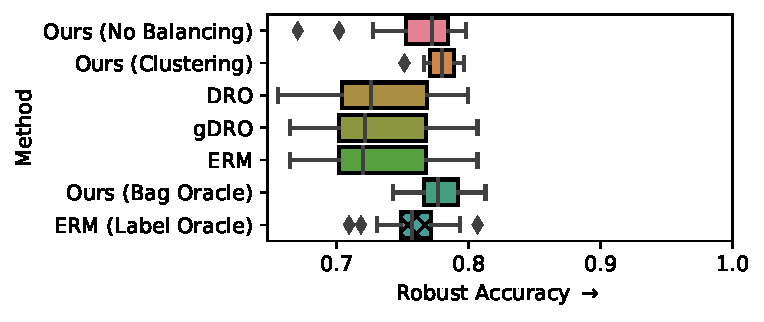
\includegraphics[width=0.49\textwidth]{supmatch/figures/adult/missing_subgroup/adult_miss_s_acc-min.pdf}
%     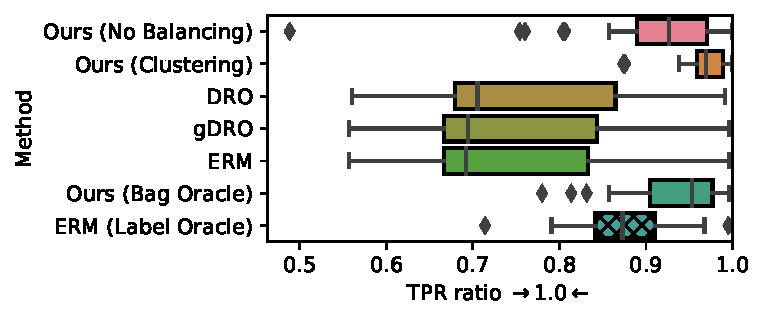
\includegraphics[width=0.49\textwidth]{supmatch/figures/adult/missing_subgroup/adult_miss_s_tprr.pdf}
%     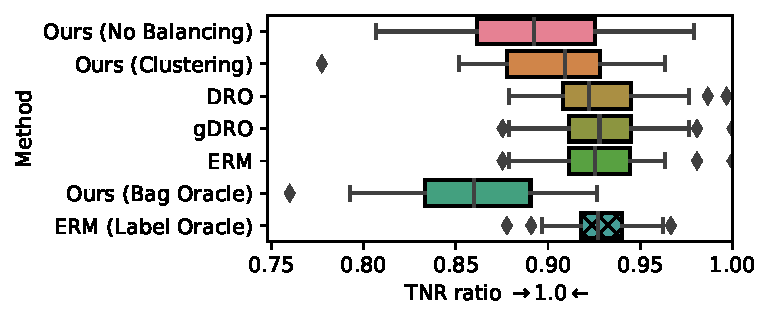
\includegraphics[width=0.49\textwidth]{supmatch/figures/adult/missing_subgroup/adult_miss_s_tnrr.pdf}
%     \caption{%
%     Results for the Adult Income dataset with a \emph{missing subgroup}, for the binary
%     classification task of predicting whether an individual earns $>$\$50,000 with a binary
%     subgrouping based on \emph{gender}.
%     \texttt{ERM (Label Oracle)} refers to a model based on ERM (empirical risk minimization),
%     trained on a \textbf{l}abeled \textbf{d}eployment set; thus not suffering from bias in the training set.
%     \textbf{Top left}: Accuracy.
%     \textbf{Top right}: Robust Accuracy.
%     \textbf{Bottom left}: True positive rate ratio.
%     \textbf{Bottom right}: True negative rate ratio.
%     For\texttt{Ours (Clustering)}, the clustering accuracy was 60.4\% $\pm$ 0.8\%.
%     % for \texttt{K-means} it was 44\% $\pm$ 3\%.
%     }%
%     \label{fig:adult-missing-subgroup}
% \end{figure*}
% Figures~\ref{fig:adult-subgroup-bias} and \ref{fig:adult-missing-subgroup} show results from our
% method on the Adult Income dataset \cite{Dua:2017}. This dataset is a common dataset for
% evaluating fair machine learning models. Each instance in the dataset is described by $14$
% characteristics including gender, education, marital status, number of work hours per week among
% others, along with a label denoting income level ($\geq$\$50K or not). We transform the
% representation into $62$ real and binary features along with the subgroup label $s$.
% %%%%%%%%CHECK THESE VALUES%%%%%%%%%%%% The dataset is naturally imbalanced with respect to
% gender: 30\% of the males are labeled as earning more than \$50K per year (high income), while
% only 11\% of females are labeled as such. For further details on the dataset construction, see
% section~\ref{ssec:dataset-construction-adult}. % Following standard practice in algorithmic
% fairness  e.g. \cite{ZemeWuSwePitetal13}, we consider gender to be the subgroup label $s$. % A
% \emph{source} is defined as certain combinations of the subgroup, $s$, and target class, $y$.

% For the Adult Income dataset, we study the following two settings of missing sources, a subgroup
% bias setting and a more extreme missing subgroup setting: 1) \emph{subgroup bias}: we have
% labeled training data for males ($s=1$) with both positive and negative outcomes, but for the
% group of females ($s=0$), we only observe the one-sided negative outcome:
% \(\mathcal{S}_{tr}(y=1)=\{1\}\); 2) \emph{missing subgroup}: we have training data for males with
% positive and negative outcomes, but do not have labeled data for females, i.e.\
% \(\mathcal{S}_{tr}(y=0)=\{1\}\) and \(\mathcal{S}_{tr}(y=1)=\{1\}\).

% As before, \texttt{Ours (Clustering)}, \texttt{Ours (No Balancing)}\ and \texttt{Ours (Bag
% Oracle)} denote variants of our method with different deployment-set balancing strategies. As
% baseline methods, we have \texttt{ERM} (standard empirical risk minimization with balanced
% batches), \texttt{DRO} \cite{HasSriNamLia18}, \texttt{gDRO} \cite{sagawa2019distributionally} and
% \texttt{ERM (Label Oracle)} which is the same model as \texttt{ERM}, but trained with access to
% the ground-truth labels of the deployment set.

% In both settings, we observe the same order as for the other dataset in terms of accuracy:
% \texttt{Ours (Bag Oracle)} achieves the highest performance, followed by \texttt{Ours
% (Clustering)}, then \texttt{Ours (No Balancing)}. However, for the \emph{missing subgroup}
% setting, \texttt{Ours (Clustering)} and \texttt{Ours (Bag Oracle)} perform almost identically,
% with the former outstripping the latter slightly in terms of de-biasing metrics. This reduced
% reliance on balancing can be explained by the additional supervision that comes with having two
% sources missing instead of one -- in order for the discriminator to distinguish between bags from
% the deployment set and bags from the training set, the former need only contain \emph{one} of the
% two missing sources.

% Generally, we observe a high variance in the results. This is not attributable to our method,
% however, with the baselines exhibiting the same behavior, but rather to the fact that the Adult
% Income dataset is a very noisy dataset which, at the best of times, allows only about 85\%
% accuracy to be attained (see also \cite{agrawal2020debiasing}). The problem is that samples vary
% widely in how informative they are. This, coupled with us artificially biasing the dataset to be
% even more biased (as \emph{subgroup bias} and \emph{missing subgroup}), makes the attainable
% performance very dependent on which samples the classifier gets to see, which varies according to
% the random seed used for the data set split.
%
\subsection{Results for 3-digit 3-colour variant of Coloured MNIST}\label{ssec:3-digit-3-color}
%
To investigate how our method scales with the number of sources, we look to a 3-digit, 3-colour
variant of the dataset in the \emph{subgroup bias} setting where four sources are missing from
$\gD^{tr}$.
Results for this configuration are shown in Fig.~\ref{fig:cmnist-3dig-4miss}. We see that the
performance of \texttt{Ours (No Balancing)} is quite close to that of \texttt{Ours (Bag Oracle)}.
We suspect this is because balancing is less critical with the increased number of subgroups
strengthening the training signal. As inter-subgroup ratios do not make for suitable metric for
non-binary $S$, we instead quantify the invariance of the predictions to the subgroup with the
\ac{HGRMC} \cite{renyi1959measures}.

\begin{figure*}[htp]
  \centering
  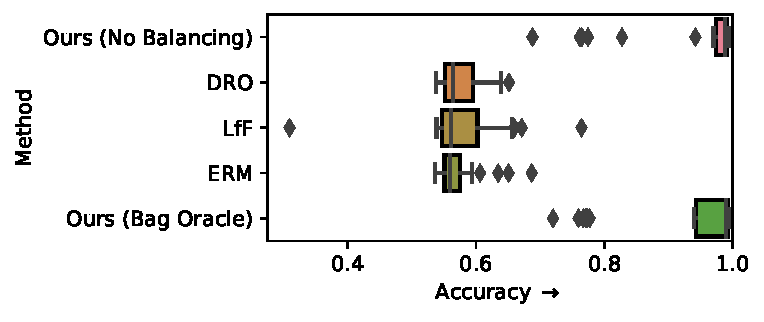
\includegraphics[width=0.49\textwidth]{supmatch/figures/cmnist/supmat/cmnist_3dig_4miss_acc.pdf}
  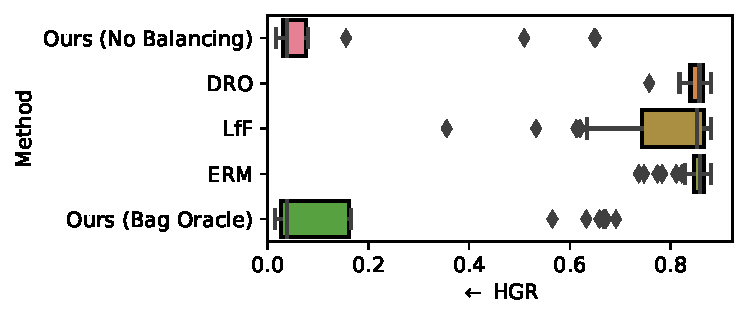
\includegraphics[width=0.49\textwidth]{supmatch/figures/cmnist/supmat/cmnist_3dig_4miss_hgr.pdf}
%   \includegraphics[width=\columnwidth]{supmatch/figures/cmnist_3dig_4miss_pr.pdf}
%   \includegraphics[width=\columnwidth]{supmatch/figures/cmnist_3dig_4miss_tpr.pdf}
%   \includegraphics[width=\columnwidth]{supmatch/figures/cmnist_3dig_4miss_tnr.pdf}
  \caption{
    Results from \textbf{30 repeats} for the Coloured MNIST dataset with three digits: `2', `4' and
    `6'. Four combinations of digit and colour are missing: {\color{green}green} 2's,
    {\color{blue}blue} 2's, {\color{blue}blue} 4's and {\color{green}green} 6's. \textbf{Left}:
    Accuracy. \textbf{Right}: Hirschfeld-Gebelein-R\'enyi maximal correlation
    \cite{renyi1959measures} between $S$ and $Y$.
  }%
  \label{fig:cmnist-3dig-4miss}
\end{figure*}
%
\subsection{Extended Results for CelebA}\label{ssec:extended-results-celeba}
%
As alluded to in main text, for three out of four of the missing gender/smiling quadrants, the
\texttt{GEORGE} baseline produced an extreme outlier for one out of the five total repeats - these
outliers were omitted from the plots to ensure the discriminability of the other results.
%
We reproduce the full, untruncated versions of these plots here in
Fig.~\ref{fig:celeba-gender-smiling-full}. We have also included \texttt{Accuracy} metric in
Fig.~\ref{fig:celeba-gender-smiling-full}.


\begin{figure*}[htp]
  \centering
  % Smiling females missing
%   \normalsize{Missing source: smiling females}\par\medskip
 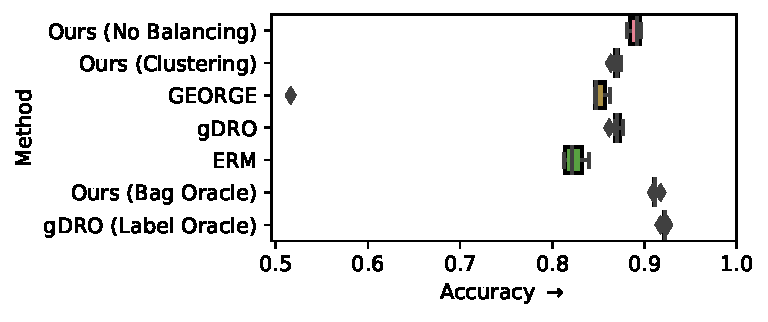
\includegraphics[width=0.49\textwidth]{supmatch/figures/celeba/supmat/no_smiling_females/celeba_gender_smiling_acc.pdf}
  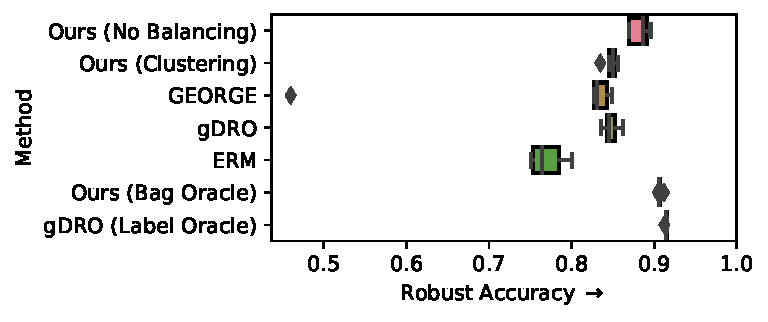
\includegraphics[width=0.49\textwidth]{supmatch/figures/celeba/supmat/no_smiling_females/celeba_gender_smiling_acc-min.pdf}
    % Smiling males missing
%   \normalsize{Missing source: smiling males}\par\medskip
 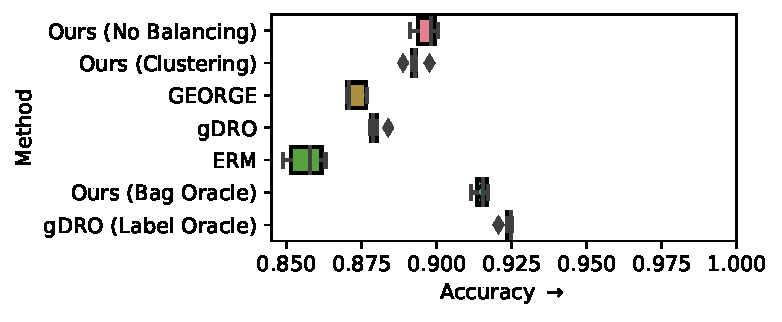
\includegraphics[width=0.49\textwidth]{supmatch/figures/celeba/supmat/no_smiling_males/celeba_gender_smiling_acc.pdf}
 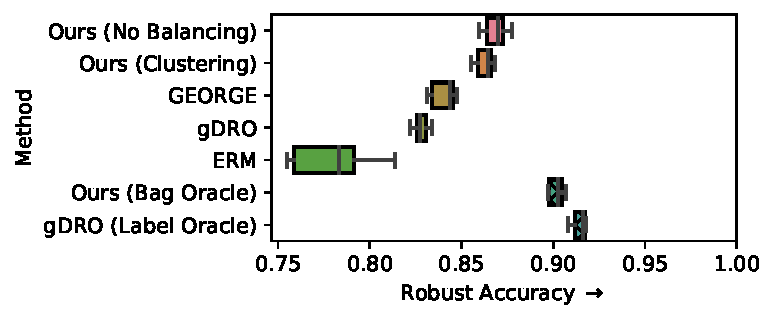
\includegraphics[width=0.49\textwidth]{supmatch/figures/celeba/supmat/no_smiling_males/celeba_gender_smiling_acc-min.pdf}
    % Unsmiling females missing
%   \normalsize{Missing source: non-smiling} females\par\medskip
 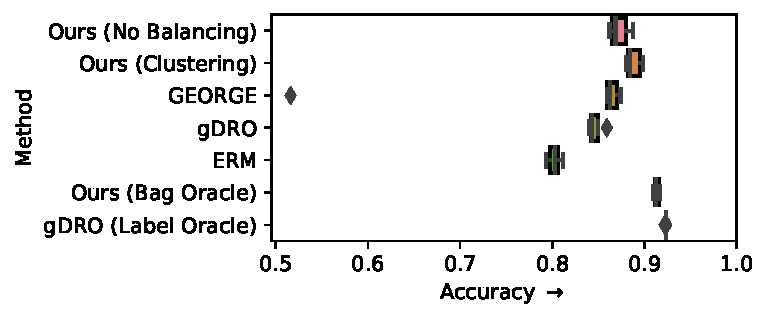
\includegraphics[width=0.49\textwidth]{supmatch/figures/celeba/supmat/no_unsmiling_females/celeba_gender_smiling_acc.pdf}
  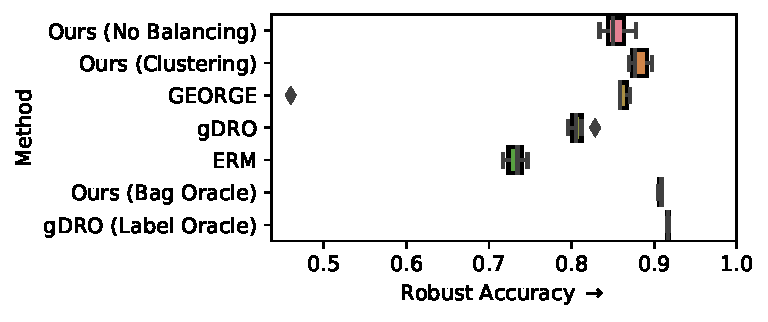
\includegraphics[width=0.49\textwidth]{supmatch/figures/celeba/supmat/no_unsmiling_females/celeba_gender_smiling_acc-min.pdf}
  % Unsmiling males missing
%   \normalsize{Missing source: non-smiling males}\par\medskip
 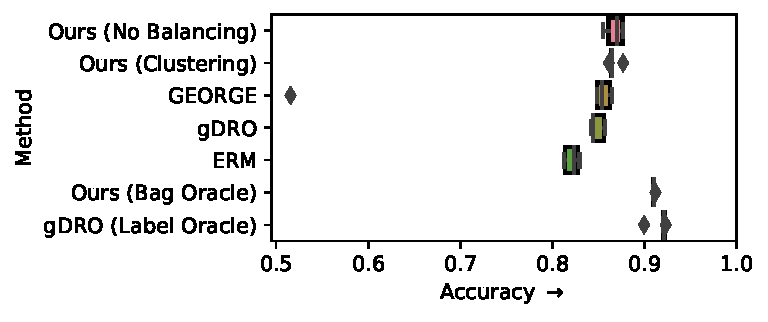
\includegraphics[width=0.49\textwidth]{supmatch/figures/celeba/supmat/no_unsmiling_males/celeba_gender_smiling_acc.pdf}
  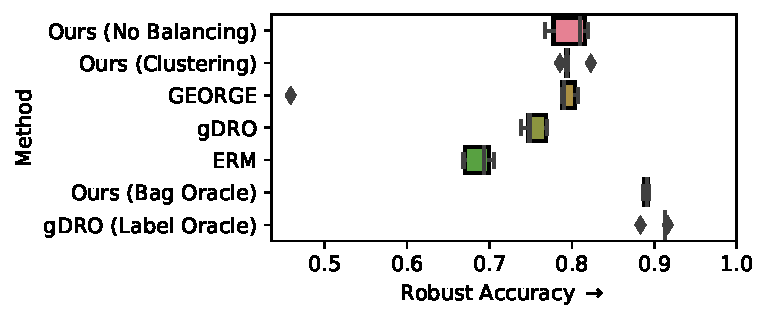
\includegraphics[width=0.49\textwidth]{supmatch/figures/celeba/supmat/no_unsmiling_males/celeba_gender_smiling_acc-min.pdf}
\caption{
    Results from \textbf{5 repeats} for the CelebA dataset for the \emph{subgroup bias} scenario.
    The task is to predict ``smiling'' vs ``non-smiling'' and the subgroups are based on gender.
    The four sources are dropped one at a time from the training set
    (\textbf{first row}: smiling females; \textbf{second row}: smiling males; \textbf{third row}:
    non-smiling females, \textbf{fourth row}: non-smiling males), while the deployment set is kept
    fixed. ``Robust Accuracy'' refers to the minimum accuracy computed over the subgroups. 
  }%
 \label{fig:celeba-gender-smiling-full}
\end{figure*}

\section{Theoretical analysis}\label{sec:theoretical-analysis}
In this section, we present our theoretical results concerning the validity of our support-matching
objective and the bound on the error introduced into it by clustering. We use notation consistent
with that used throughout the main text.

\subsection{Sampling function for the objective}%
\label{sub:sampling_function_for_objective}
The stated objective uses the following helper function:
\begin{align}
\Pi(s',y') = \begin{cases}
  \{s'\}&\text{if }\,\gS^{tr}_{Y=y\prime}=\gS\\
  \gS^{tr}_{Y=y'}&\text{otherwise}~.
\end{cases}
\end{align}
This helper function determines which $s$ value in the training set an $s$-$y$ pair from the
deployment set is mapped to. (The $y$ value always stays \emph{the same} when mapping from
deployment set to training set.) To demonstrate the usage of this function, we consider the example
of binary Coloured MNIST with \(\gS=\{\text{\color{purple}{purple}}, \text{\color{green}green}\}\)
and \(\gY=\{2, 4\}\) where the training set is missing \((s=\text{purple}, y=4)\). In this case,
$\Pi$ takes on the following values:
\begin{align}
  \Pi(\text{{\color{purple}purple}}, 2) &= \{\text{\color{purple}purple}\}\\
  \Pi(\text{\color{green}green},  2) &= \{\text{\color{green}green} \}\\
  \Pi(\text{\color{purple}purple}, 4) &=\gS^{tr}_{y=4} = \{\text{\color{green}green} \}\\
  \Pi(\text{\color{green}green},  4) &=\gS^{tr}_{y=4} = \{\text{\color{green}green} \}
\end{align}
% See also figure \ref{fig:matching-repeated} which is a visualization of this.
It is essential that \((s=\text{\color{purple}{purple}}, y=4)\) from the deployment set is mapped
to \((s=\text{\color{green}{green}}, y=4)\) from the training set, and not
\((s=\text{\color{purple}{purple}}, y=2)\).
% The latter would produce an invariance to $y$, which is undesirable.
This procedure is illustrated in Fig.~\ref{fig:matching-repeated-correct}, and contrasted with an
incorrect procedure based on balancing the bag according to $s$ in
\ref{fig:matching-repeated-incorrect} -- such a procedure would result in invariance to $y$ instead
of $s$, which is obviously undesirable.

In practice, we use the following sampling function $\pi$ to implement $\Pi$, sampling from it for
all $(s,y) \in S \times Y$:
%
\begin{align}
  \pi(s',y') = \begin{cases} x\sim P^\mathit{tr}(x|S=s',y'), \\
    \quad\quad\quad\quad\quad\quad\quad\quad\text{if }\,\gS^{tr}_{Y=y'}=\gS \\
  x\sim P^\mathit{tr}(x|s=\check{s},y'), \check{s}\sim \mathrm{uniform}(S^{tr}), \\
    \quad\quad\quad\quad\quad\quad\quad\quad\text{otherwise}~.
\end{cases}
\label{eq:functional-sampling}
\end{align}
%
With the assumption that our data follows a two-level hierarchy and all digits appear in the
training set, the above sampling function $\pi$ traverses the first level which corresponds to the
class-level information, and \emph{samples} the second level which corresponds to subgroup-level
information when we have missing sources.
 
% ensures that the bags from the training set only differ from those from the deployment set where
% a source is missing; and furthermore, that they only differ in $s$, but not in $y$.

\begin{figure}[htp]
  \begin{subfigure}{0.49\textwidth}
    \centering
    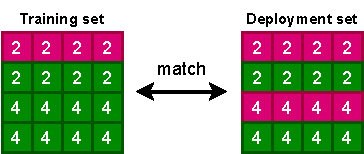
\includegraphics[width=0.9\linewidth]{supmatch/figures/illustrations/matching_diagram.pdf}
    \caption{Correct matching procedure.}%
    \label{fig:matching-repeated-correct}
  \end{subfigure}
  \begin{subfigure}{0.49\textwidth}
    \centering
    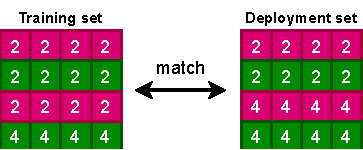
\includegraphics[width=0.9\linewidth]{supmatch/figures/illustrations/y-inv.pdf}
    \caption{\emph{In}correct matching procedure.}%
    \label{fig:matching-repeated-incorrect}
  \end{subfigure}
  \caption{%
    The two natural matching procedures for one missing source in the training set.
    Only figure \ref{fig:matching-repeated-correct} (left) produces the desired invariance.
  }%
  \label{fig:matching-repeated}
\end{figure}


% Sampling from $\pi (s,y)$ for all $(s,y) \in S \times Y$ ensures that the bags from the training
% set only differ from those from the deployment set where a source is missing; and furthermore,
% that they only differ in $s$, but not in $y$. For example, if the bag size is four, $\gY$ and
% $\gS$ are binary, and the combination $(y=1,s=0)$ is missing, then each bag should contain two
% samples of $(y=1,s=1)$ and one sample each for $(y=0,s=0)$ and $(y=0,s=1)$. e.

\subsection{Implication of the objective}\label{implication-of-the-objective}
We restate proposition 1 and present the proof.

We prove here that an encoding $f$ satisfying the objective is invariant to \(s\), at least in
those cases where the class does not have full \(s\)-support (which is exactly the case where it
matters).

\begin{theorem}
If \(f\) is such that
\begin{align}
p_f|_{s\in \Pi(s',y'),Y=y'} = q_f|_{S=s',Y=y'}\quad\forall s'\in\gS, y' \in\gY
\end{align}
%
and \(P^\mathit{tr}\) and \(P^\mathit{dep}\) are data distributions that correspond to the real
data distribution \(P\), except that some \(s\)-\(y\)-combinations are less prevalent, or, in the
case of \(P^\mathit{tr}\), missing entirely, then, for every \(y'\in\gY\), there is either full
coverage of \(s\) for \(y'\) in the training set (\(\gS^{tr}_{Y=y\prime}=\gS\)), or the following
holds:
%
\begin{align}
P(S=s'|f(X)=z', Y=y')=\frac{1}{n_s}~.
\end{align}
%
In other words: for \(Y=y'\), \(f(x)\) is not predictive of \(s\).
\end{theorem}

\begin{proof}
If \(y'\) has full coverage of \(s\) in the training set, there is nothing to prove.
%
So, assume \(y'\) does not have full \(s\)-support.
%
That means \(\Pi(s',y')=\gS^{tr}_{Y=y\prime} \) for all \(s'\in \gS\).
%
And so
%
\begin{align}
&P^\mathit{tr}(f(X)=z'|s\in \gS^{tr}_{Y=y\prime}, Y=y')\\
  =\;&P^\mathit{dep}(f(X)=z'|S=s', Y=y')\quad\quad\quad\quad\forall s'\in\gS \nonumber
\end{align}
%
The left-hand side of this equation does not depend on \(s'\)
and so the right-hand side must have the same value for all \(s'\in\gS\), which implies:
\begin{align}
&P^\mathit{dep}(f(X)=z'|S=s', Y=y') \nonumber\\
  =\;&P^\mathit{dep}(f(X)=z'|Y=y')
\end{align}
%
Now, by assumption, the different data distributions \emph{train} and \emph{deployment} only differ
from the ``true'' distribution by the prevalence of the different \(s\)-\(y\)-combinations, with
the \emph{deployment} data distribution having all combinations but potentially not in equal
quantity. However, as we restrict ourselves to a certain combination (\(S=s',Y=y'\)) in the above
equation, the equation also holds in the true data distribution:
%
\begin{align}
&P(f(X)=z'|S=s', Y=y') \nonumber\\
=\;&P(f(X)=z'|Y=y')
\end{align}
%
Then, using Bayes' rule, we get
%
\begin{align}
&P(S=s'|f(X)=z', Y=y') \nonumber\\
=\;&\frac{P(f(X)=z'|S=s', Y=y')P(S=s'|Y=y')}{P(f(X)=z'|Y=y')} \nonumber\\
=\;&P(S=s'| Y=y')~.
\end{align}
%
Finally, in the true data distribution, we have a uniform prior:
\(P(S=s'|Y=y')=(n_s)^{-1}\). This concludes the proof.
\end{proof}
%
\subsection{Bound on error introduced by clustering}\label{bound-on-error-introduced-by-clustering}
%
As previously stated, in practice, no labels are available for the deployment set.
Instead, we identify the relevant groupings by clustering.
Such clustering cannot be expected to be perfect.
So, how will clustering affect the calculation of our objective?

\begin{theorem}
  %
If \(q_f(Z)\) is a data distribution on \(\mathcal{Z}\) that is a mixture of \(n_y\cdot n_s\)
Gaussians, which correspond to all unique combinations of \(y\in\gY\) and \(s\in\gS\), and
\(p_f(Z)\) is any data distribution on \(\mathcal{Z}\), then without knowing \(y\) and \(s\) on
\(q_f\), we can estimate
%
\begin{align}
\sum\limits_{s'\in\gS}\sum\limits_{y'\in\gY} TV(p_f|_{s\in \Pi(s',y'),Y=y'}, q_f|_{S=s',Y=y'})
\end{align}
%
with an error that is bounded by \(\tilde{O}(\sqrt{1/N})\) with high probability, where \(N\) is
the number of samples drawn from \(q_f\) for learning.
%
\end{theorem}

\begin{proof}
First, we produce an estimate \(\hat{q}_f\) of \(q_f\) using the algorithm from
\cite{ashtiani2020near}, which gives us a mixture-of-Gaussian distribution of \(n_y\cdot n_s\)
components with \(TV(q_f, \hat{q}_f)\leq \tilde{O}(\sqrt{1/N})\) with high probability, where \(N\)
is the number of data points used for learning the estimate. Then, by Lemma 3 from
\cite{SohDunAngGuetal20}, \emph{there exists} a mapping \(i\) from the components \(k\) of the
Gaussian mixture \(\hat{q}_f\) to the \(s\)-\(y\)-combinations in \(q_f\) such that
%
\begin{align}
&TV(q_f(Z|S=s',Y=y'),\hat{q}_f(Z|k=i(s',y'))) \\
&\quad\quad\quad\quad\quad\quad\quad\quad\quad\quad\quad\quad\quad\quad\leq
\tilde{O}\left(\frac{1}{\sqrt{N}}\right)~. \nonumber
\end{align}
%
Now, consider the element of the sum in the objective that corresponds
to \((s',y')\):
%
\begin{align}
&TV(p_f(Z|s\in \Pi(s',y'),Y=y'), q_f(z|S=s',Y=y'))\nonumber\\
\leq \;&TV(p_f(Z|s\in \Pi(s',y'),Y=y'), \hat{q}_f(Z|k=i(s',y')))\nonumber\\
&\quad\quad+TV(\hat{q}_f(z|k=i(s',y')), q_f(z|S=s',Y=y'))\nonumber\\
\leq \;&TV(p_f(Z|s\in \Pi(s',y'),Y=y'), \hat{q}_f(Z|k=i(s',y'))) \nonumber\\
&\quad\quad+\tilde{O}(1/\sqrt{N})
\end{align}
%
Thus, for the whole sum over \(s\) and \(y\), the error is bounded by
\begin{align}
\sum\limits_{s'\in\gS}\sum\limits_{y^\prime\in\gY}\tilde{O}(\sqrt{1/N})
\leq n_sn_y \max\limits_{(s',y')\in\gS\times\gY}\tilde{O}(\sqrt{1/N})
\end{align}
which is equivalent to just \(\tilde{O}(\sqrt{1/N})\).
\end{proof}
%
\section{Dataset Construction}\label{sec:dataset-construction}
%
\subsection{Coloured MNIST and biasing parameters}
%
The MNIST dataset \cite{lecun1998gradient} consists of 70,000 (60,000 designated for training,
10,000 for testing) images of grey-scale hand-written digits. We colour the digits following the
procedure outlined in \cite{KehBarThoQua20}, randomly assigning each sample one of ten distinct RGB
colours. Each source is then a combination of digit-class (class label) and colour (subgroup label).
We use no data-augmentation aside from symmetrically zero-padding the images to be of size 32x32.
% To simulate a more realistic setting, we create artificial imbalance in both $\gD_{dep}$ and
% $\gD^{tr}$ by sub-sampling the remaining sources. 
%The sub-sampling proportions used for each set of experiments can be found in Appendix E.

%\subsection{Coloured MNIST biasing parameters}
To simulate a more real-world setup where the data, labelled or otherwise, is not naturally
balanced, we bias the Coloured MNIST training and deployment sets by downsampling certain
colour/digit combinations. The proportions of each such combination \emph{retained} in the
\emph{subgroup bias} (in which we have one source missing from the training set) and \emph{missing
subgroup} (in which we have two sources missing from the training set) are enumerated in
table~\ref{color_mnist_biasing_po} and \ref{color_mnist_biasing_id}, respectively. For the
3-digit-3-colour variant of the problem, no biasing is applied to either the deployment set or the
training set (the missing combinations are specified in the caption accompanying
figure~\ref{fig:cmnist-3dig-4miss-add}); this variant was experimented with only under the
subgroup-bias setting.

\begin{table}[ht]
\caption{Biasing parameters for the training (left) and deployment (right) sets of Coloured MNIST in
the \emph{subgroup bias} setting.}
\label{color_mnist_biasing_po}
\centering
\begin{tabular}{lcc}
\toprule
Combination   & \multicolumn{2}{c}{Proportion retained} \\ \cmidrule(lr){2-3}
  & training set & deployment set \\ \midrule
(Y = 2, S = {\color{purple}purple}) & 1.0  & 0.7 \\
(Y = 2, S = {\color{green}green})   & 0.3  & 0.4 \\
(Y = 4, S = {\color{purple}purple}) & 0.0  & 0.2 \\
(Y = 4, S = {\color{green}green})   & 1.0  & 1.0 \\
\bottomrule
\end{tabular}
\end{table}

\begin{table}[ht]
\caption{Biasing parameters for the training (left) and deployment (right) sets of Coloured MNIST in
the \emph{missing subgroup} setting.}
\label{color_mnist_biasing_id}
\centering
\begin{tabular}{lcc}
\toprule
Combination   & \multicolumn{2}{c}{Proportion retained} \\ \cmidrule(lr){2-3}
  & training set & deployment set \\ \midrule
(Y = 2, S = {\color{purple}purple}) & 0.0  & 0.7 \\
(Y = 2, S = {\color{green}green})   & 0.85 & 0.6 \\
(Y = 4, S = {\color{purple}purple}) & 0.0  & 0.4 \\
(Y = 4, S = {\color{green}green})   & 1.0  & 1.0 \\
\bottomrule
\end{tabular}
\end{table}

% \subsection{Adult Income biasing parameters}\label{ssec:dataset-construction-adult}
% For the Adult Income dataset, we do not need to apply any synthetic biasing as the dataset
% naturally contains some bias w.r.t. $s$. Thus, we instantiate the deployment set as just a random
% subset of the original dataset. However, explicit balancing of the test set \emph{is} needed to
% yield meaningful evaluation (namely through the penalizing of biased classifiers) but care needs
% to be taken in doing so. Balancing the test set such that
% \begin{align}
%     |\{x \in X |s=0, y=0\}| &= |\{x \in X |s=1, y=0\}|    \nonumber\\
%     \text{and}~|\{x \in X |s=0, y=1\}| &= |\{x \in X |s=1, y=1\}|
% \end{align}
% where for both target classes, $y=0$ and $y=1$, the proportions of the groups $s=0$ and $s=1$ are
% made to be the same, is intuitive, yet at the same time precludes sensible comparison of the
% accuracy/fairness trade-off of the different classifiers. Indeed, with the above conditions, a
% majority classifier (predicting all 1s or 0s) achieves comparable accuracy to the
% fairness-unaware baselines, while also being perfectly fair by construction.
% This observation motivated us to devise an alternative scheme, where we balance the test set
% according to the following constraints
% \begin{align}
%     & |\{x \in X |s=0, y=0\}| 
%     = |\{x \in X |s=0, y=1\}|  \nonumber \\
%     = &|\{x \in X |s=1, y=1\}|
%     = |\{x \in X |s=1, y=0\}|~.
%  \end{align}
% That is, all subsets of $\gS \times \gY$ are made to be equally sized. Under this new scheme the
% accuracy of the the majority classifier is 50\% for the binary-classification task.

\section{Model details and optimization}
\subsection{Overview of model architecture}\label{sec:model-arch}
\begin{figure*}[htp]
    % \begin{subfigure}{0.74\textwidth}
    \centering
    %
\includegraphics[width=0.9\textwidth]{supmatch/figures/SSL-framework}
    % 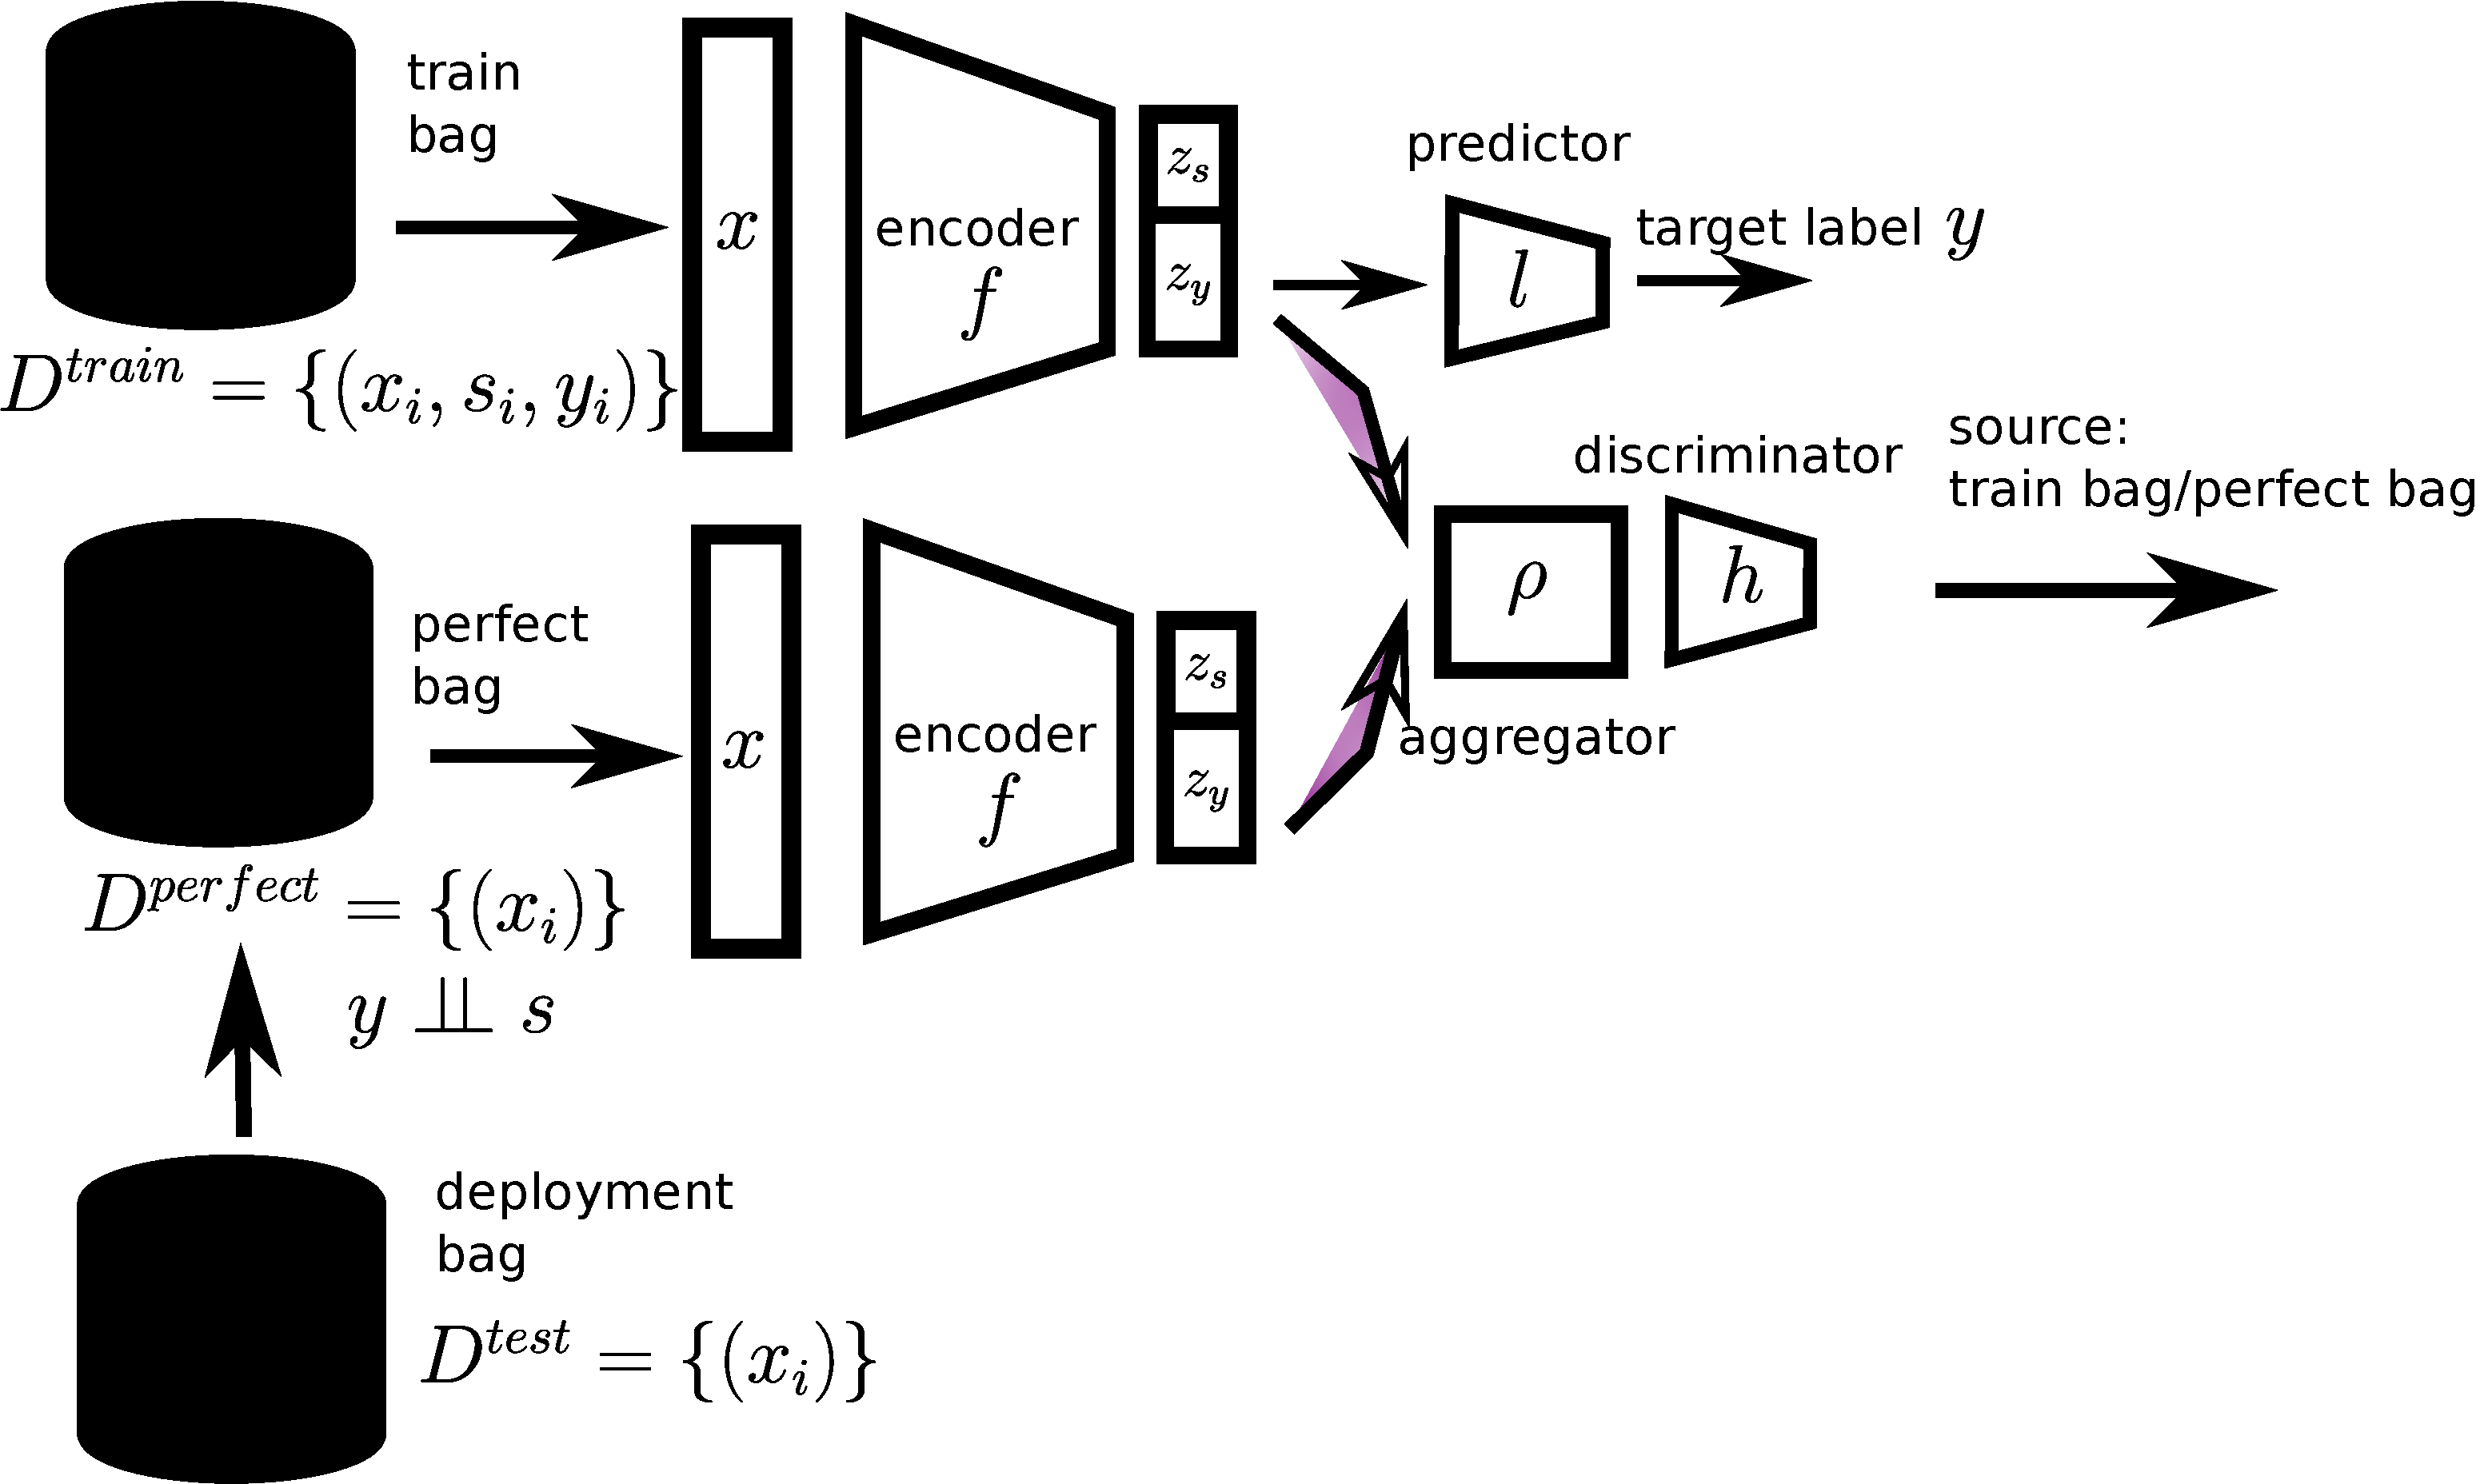
\includegraphics[width=\textwidth]{supmatch/figures/SSL-framework-withPred.pdf}
    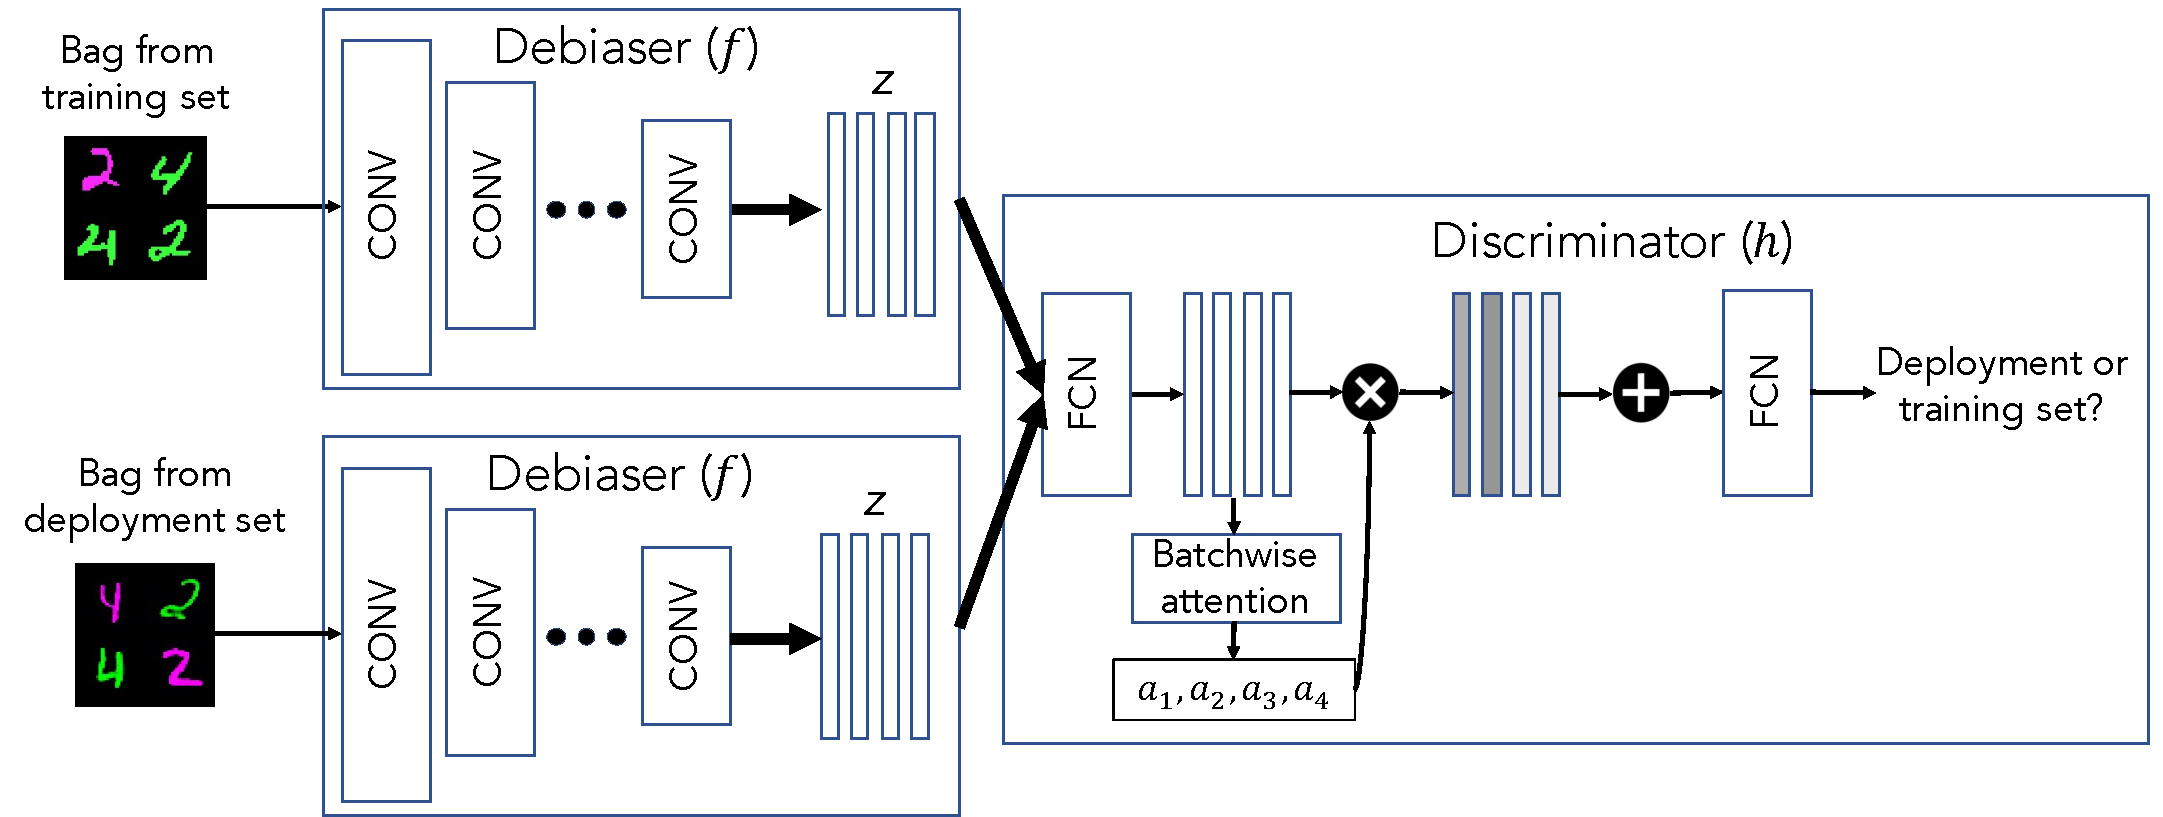
\includegraphics[width=\textwidth]{supmatch/figures/illustrations/architecture.pdf}
    \caption{% The main components of our support-matching algorithm, $f$ (debiaser) and $h$
      (discriminator). The debiaser is trained to produce encodings, $z$ of the data that are
      invariant to the subgroups differences. %source dataset and thereby the subgroups identifying
      it. In order to determine whether a bag of encodings originates from the training set or the
      deployment set, the discriminator performs an attention-weighted aggregation over the bag
      dimension to model interdependencies between the samples. In the case of Coloured MNIST where
      {\color{purple}purple} fours constitute the missing subgroup, the discriminator can identify
      an encoding of a bag from the training set by the absence of such samples as long as color
      information is detectable in $z$. %, thereby serving as an error signal for the debiaser. By
    learning a subgroup invariant representation, the debiaser can hide the origin of the bags from
  the discriminator.} \label{fig:architecture}
\end{figure*}%
%
We give a more detailed explanation of the model used in our method.
Fig.~\ref{fig:architecture} shows the core of our method:
the debiaser, $f$, which produces bags of encodings, $z$
-- on both the training and the deployment set --
which are then fed to a discriminator that tries to identify the origin of the bags.
The discriminator uses batch-wise attention in order to consider a bag as a whole,
which allows cross-comparisons.
%
\subsection{Details of the attention mechanism}\label{ssec:attention-mechanism}
%
The \emph{discriminator} function $h$ that predicts which dataset a bag of samples embedded in $z$
was sampled from should have the following property: \( h((f(x) | x \in B)) = h((f(x) | x \in \pi
(B))) \) for all permutations $\pi$, and $f: x \to z$. 
%
For the entirety of function $h$ -- composed of sub-functions \( h_1(h_2(h_3...))) \) -- to have this
property, it suffices that only the innermost sub-function, $\rho$, does. 
%
While there are a number of choices when it comes to defining $\rho$, we choose a weighted average
$\rho = \frac{1}{|\mathcal{B}|} \sum_{x \in B}\mathrm{attention}(f(x), B) \cdot f(x)$, with weights
computed according to a learned attention mechanism. 
%
The idea of using an attention mechanism for set-wise classification has been previously explored
to great success by, e.g., \cite{lee2019set}. %\cite{ilse2018attention} and \cite{lee2019set}. 
%
We employ an bag-wise attention mechanism based on the scaled dot-product attention of
\cite{vaswani2017attention}, where in our case we define $K$ and $V$ to be linear projections of
$z$ -- $zW_k$ and $zW_v$, respectively -- and $Q$ to be mean of another linear projection of $z$,
$zW_q$, taken over the bag dimension.

\begin{align*}
  \text{Attention}(\mathit{Q}, \mathit{K}, \mathit{V}) := \text{Softmax} \biggl( \frac{ \mathit{Q}
  \mathit{K}^T  } { \sqrt{d} } \biggr) V
\end{align*}

The output of $\rho$ is then further processed by a series of fully-connected layers and the final
output is the binary prediction for a given bag of samples.

\subsection{Training procedure and hyperparameters}
\begin{table*}[tp]
 \centering
 \caption{Selected hyperparameters for experiments with Coloured MNIST, Adult and CelebA datasets.}
 \label{tab:hparams}
 \scalebox{0.8}{
 \begin{tabular}{llll}
 \toprule
 & \textbf{Coloured MNIST} & \textbf{Adult} & \textbf{CelebA}       
 \\ & 2-dig SB / 2-dig MS / 3-dig SB
 \\ \midrule
 Input size  &   $3 \times 32 \times 32$ & $61$ & $3 \times 64 \times 64$ \\  \midrule
 \multicolumn{4}{c}{AutoEncoder}                     \\ \midrule
 Levels                      & $4$         & $1$    & $5$\\
 Level depth                 & $2$         & $1$    & $2$\\
 Hidden units / level        & $[32, 64, 128, 256]$ & $[61]$ & $[32, 64, 128, 256, 512]$\\
 Activation                  & GELU        & GELU   & SiLU  \\
 Layer-wise Normalisation               & -           & -      & LayerNorm \\
 Downsampling op.  & Strided Convs. & -- & Strided Convs.\\
 Reconstruction loss         & MSE         & Mixed$^1$  & MSE \\
 Learning rate               & $1 \times 10^{-3}$   & $1 \times 10^{-3}$  & $1 \times 10^{-3}$ \\ \midrule
 \multicolumn{4}{c}{Clustering}                      \\ \midrule
 Batch size                  & $256$      & $1000$  & $256$ \\
 AE pre-training epochs      & $150$        & $100$ & $10$  \\
 Clustering epochs           & $100$       & $300$  & $20$ \\
 Self-supervised loss & Cosine + BCE & Cosine + BCE & Cosine \\
 U (for ranking statistics)             & $5$         & $3$     & $8$    \\   \midrule
 \multicolumn{4}{c}{Support-Matching}                   \\ \midrule
 Batch size & $1$/$32$/$14$  & $64$   & $32$ \\
 Bag size   & $256$/$8$/$18$ & $32$ & $8$ \\
 Training iterations    & $8\text{k}/8\text{k}/20\text{k}$ & $5\text{k}$ & $2\text{k}$ \\
 Encoding ($z$) size$^2$  & $128$   & $35$  & $128$ \\
 Binarised $\tilde{s}$ & \xmark\, / \cmark\, / \cmark & \xmark & \xmark \\
 $y$-predictor weight ($\lambda_1$) & $1$ & $0$ & $1$  \\ 
 $s$-predictor weight ($\lambda_2$) & $1$ & $0$ & $1$  \\ 
 Adversarial weight ($\lambda_3$)   & $1 \times
 10^{-3}$   & $1$   & $1$\\ 
 Stop-gradient $\left(\nabla_\theta h_\psi(f_\theta(X^\mathit{dep}))=0\right)$ & \xmark & \cmark & \xmark \\
 \midrule
 \multicolumn{4}{c}{Predictors}   \\ \midrule
 Learning rate  & $3 \times 10^{-4}$ &   $1 \times 10^{-3}$  $ 1 \times 10^{-3}$\\
 \midrule
 \multicolumn{4}{c}{Discriminator}                   \\ \midrule
 Attention mechanism$^3$    & Gated   & Gated & Gated \\
 Hidden units pre-aggregation  & $[256, 256]$  & $[32]$ & $[256, 256]$\\
 Hidden units post-aggregation & $[256, 256]$ & --  & $[256, 256]$ \\
 Embedding dim (for attention) & $32$ & $128$ & $128$ \\
 Activation & GELU & GELU & GELU \\
 Learning rate  & $3 \times 10^{-4}$    & $1 \times 10^{-3}$ & $1 \times 10^{-3}$\\
 Updates / AE update    & $1$  & $3$    & $1$    \\
 \bottomrule
 \addlinespace
 \multicolumn{4}{p{17cm}}{\footnotesize $^1$ Cross-entropy is used for categorical features, MSE for continuous features.} \\
 \multicolumn{4}{p{17cm}}{\footnotesize $^2$ $|z|$ denotes the combined size of $\tilde{s}$ and
 $z$, with the former occupying $\ceil{\text{log}_2(\gS)}$ dimensions, the latter the remaining dimensions.} \\
 \multicolumn{4}{p{17cm}}{
 \footnotesize $^3$ 
 The attention mechanism used for computing the sample-weights within a bag. \emph{Gated} refers to
 gated attention  proposed by \cite{ilse2018attention}, while \emph{SDP} refers to the scaled
 dot-product attention proposed by \cite{vaswani2017attention}.
 }
 \end{tabular}
 }
 % add empty lines to make the table take up a full page
 ~\\
 ~\\
 ~\\
\end{table*}

The hyperparameters and architectures for the \acf{AE} (\texttt{AE}), Predictor and Discriminator
sub-networks are detailed in Table \ref{tab:hparams} for all three datasets.We train all models
using \texttt{Adam} \cite{KinBa15}.

For the Coloured MNIST and CelebA datasets, the baseline \texttt{ERM}, \texttt{DRO}, \texttt{LfF}
(in the case of the former) and \texttt{gDRO} (in the case of the latter) models use a
convolutional backbone consisting of one Conv-BN-LReLU block per ''stage``, with each stage
followed by max-pooling operation to spatially downsample by a factor of two to produce the
subsequent stage. This backbone consists of 4 and 5 stages for Coloured MNIST and CelebA,
respectively. The output of the backbone is flattened and fed to a  single fully-connected layer of
size $|Y|$ in order to obtain the class-prediction, $\hat{y_i}$, for a given instance. To evaluate
our method, we simply train a linear classifier on top of $z$; this is sufficient due to
linear-separability being encouraged during training by the $y$-predictor. For the Adult Income
dataset, we use an \ac{MLP} composed of a single hidden layer 35 units in size, followed by a SELU
activation \cite{klambauer2017self}, as both the downstream classifier for our method, and as the
network architecture of the baselines. All baselines and downstream classifiers alike were trained
for $60$ epochs with a learning rate of $1 \times 10^{-3}$ and a batch size of $256$.

Since, by design, we do not have labels for all subgroups the model will be tested on, and bias
against these missing subgroups is what we aim to combat, properly validating, and thus conducting
hyperparameter selection for models generally, is not straightforward. Indeed, performing
model-selection for domain generalisation problems is well-known to be a difficult problem
\cite{gulrajani2021search}. We can use estimates of the mutual information between the
learned-representation and $s$ and $y$ (which we wish to minimize w.r.t.\ to the former, maximise
w.r.t.\ the latter) to guide the process, though optimizing the model w.r.t.\ to these metrics
obtained from only the training set does not guarantee generalisation to the missing subgroups. We
can, however, additionally measure the entropy of the predictions on the encoded test set and seek
to maximise it across all samples, or alternatively train a discriminator of the same kind used for
distribution matching as a measure of the shift in the latent space between datasets. We use the
latter approach (considering the combination of the learned distance between subspace distributions
and reconstruction loss) to inform an extensive grid-search over the hyperparameter space for our
method.

For the \texttt{DRO} baseline, we allowed access to the labels of the test set for the purpose of
hyperparameter selection, performing a grid-search over multiple splits to avoid overfitting to any
particular instantiation. Specifically, the threshold ($\eta$) parameter for \texttt{DRO} was
determined by a grid-search over the space $\{0.01, 0.1, 0.3, 1.0\}$.

% In addition to the losses stated in the support-matching objective, $\mathcal{L}$, in the main
% text, we also regularize the encoder by the $\ell^2$ norm of its embedding, multiplied by a small
% pre-factor, finding this to work better than more complex regularization methods, such as spectral
% normalization \cite{miyato2018spectral}, for stabilizing adversarial training. \section{Additional
% analysis of results}\label{sec:additional-analysis}

\subsection{Visualisations of results}\label{sec:qual-results}
\begin{figure}[tp]
  \centering
  \begin{subfigure}[b]{0.49\columnwidth}
    \centering
    % 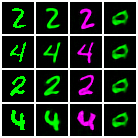
\includegraphics[width=\textwidth]{supmatch/example_images/fresh-dawn-2179_train_reconstructions_9900.png}
    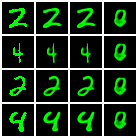
\includegraphics[width=\textwidth]{supmatch/example_images/copper-microwave-2174_train_reconstructions_9900.png}
    \caption{
    Different reconstructions on the training set. Corresponding to: original, full reconstruction,
    reconstruction of $z$ ($\tilde{s}$ zeroed out), reconstruction of $\tilde{s}$ ($z$ zeroed out).
    }%
    \label{fig:cmnist-recon-training}
  \end{subfigure}
   \hfill
%   \quad
  \begin{subfigure}[b]{0.49\columnwidth}
    \centering
    % 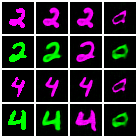
\includegraphics[width=\textwidth]{supmatch/example_images/fresh-dawn-2179_context_reconstructions_9900.png}
    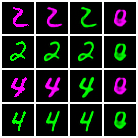
\includegraphics[width=\textwidth]{supmatch/example_images/copper-microwave-2174_context_reconstructions_9900.png}
    \caption{
    Different reconstructions on the deployment set. Corresponding to: original, full
    reconstruction, reconstruction of $z$ ($\tilde{s}$ zeroed out), reconstruction of $\tilde{s}$
    ($z$ zeroed out).
    }%
    \label{fig:cmnist-recon-deployment}
  \end{subfigure}
  \caption{
   Visualisation of our method's solutions for the Coloured MNIST dataset, with
   {\color{purple}purple} as the missing subgroup. In each of the subfigures
   \ref{fig:cmnist-recon-training} and \ref{fig:cmnist-recon-deployment}: Column 1 shows the
   original images from $x$ from the respective set. Column 2 shows plain reconstructions generated
   from $x_\textit{recon}=g(f(x), t(x))$. Column 3 shows reconstruction with zeroed-out
   $\tilde{s}$: $g(f(x), 0)$, which effectively visualizes $z$. Column 4 shows the result of an
   analogous process where $z$ was zeroed out instead.
  }%
  \label{fig:cmnist-recon}
\end{figure}%
%
\begin{figure}[tp]
  \centering
  \begin{subfigure}[b]{0.49\columnwidth}
    \centering
    \includegraphics[width=\textwidth]{supmatch/example_images/zany-glade-2191_train_reconstructions_9900.png}
    \caption{
    Different reconstructions on the training set. Corresponding to: original, full reconstruction,
    reconstruction of $z$ ($\tilde{s}$ zeroed out), reconstruction of $\tilde{s}$ ($z$ zeroed out).
    }%
    \label{fig:cmnist-recon-training-failure}
  \end{subfigure}
   \hfill
%   \quad
  \begin{subfigure}[b]{0.49\columnwidth}
    \centering
    \includegraphics[width=\textwidth]{supmatch/example_images/zany-glade-2191_context_reconstructions_9900.png}
    \caption{
    Different reconstructions on the deployment set. 
    %
    Corresponding to: original, full reconstruction, reconstruction of $z$ ($\tilde{s}$ zeroed
    out), reconstruction of $\tilde{s}$ ($z$ zeroed out).
    }%
    \label{fig:cmnist-recon-deployment-failure}
  \end{subfigure}
  \caption{
    %
   Visualisation of a failure of our method for the Coloured MNIST dataset, with
   {\color{purple}purple} as the missing subgroup. 
   %
   In each of the subfigures \ref{fig:cmnist-recon-training-failure} and
   \ref{fig:cmnist-recon-deployment-failure}: Column 1 shows the original images from $x$ from the
   respective set. Column 2 shows plain reconstructions generated from $x_\textit{recon}=g(f(x),
   t(x))$. Column 3 shows reconstruction with zeroed-out $\tilde{s}$: $g(f(x), 0)$, which
   effectively visualises $z$. Column 4 shows the result of an analogous process where $z$ was
   zeroed out instead.
   %
  }%
  \label{fig:cmnist-recon-failure}
\end{figure}%
%
\begin{figure}[htp]
     \centering
     \includegraphics[width=0.5\textwidth]{supmatch/example_images/reconstructions_celeba.png}
     \caption{%
       %
       Visualisation of our method's solutions for the CelebA dataset, with ``smiling females'' as
       the missing subgroup. 
     %
       Column 1 shows the original images from $x$ from the deployment set of CelebA. 
     %
       Column 2 shows plain reconstructions generated from $x_\textit{recon}=g(f(x), t(x))$.
     %
       Column 3 shows reconstruction with zeroed-out $\tilde{s}$: $g(f(x), 0)$, which effectively
       visualises $z$. 
     %
       Column 4 shows the result of an analogous process where $z$ was zeroed out instead.
     %
     }%
     \label{fig:celeba-recons}
\end{figure}%
%
\begin{figure*}[htp]
  \centering
    \begin{subfigure}[b]{0.49\textwidth}
    \includegraphics[width=\textwidth]{supmatch/figures/celeba_attn_map.png}
    \end{subfigure}
    \hfill
    \begin{subfigure}[b]{0.49\textwidth}
    \includegraphics[width=\textwidth]{supmatch/figures/cmnist_attn_map.png}
    \end{subfigure}
  \caption{
    Example sample-wise attention maps for bags of CelebA (left) and CMNIST (right) images sampled
    from a balanced deployment set. 
    %
    The training set is biased according to the \emph{subgroup bias} setting where for CelebA
    ``smiling females'' constitute the missing source and for Coloured MNIST {\color{purple}purple}
    fours constitute the missing source. 
    %
    The attention weights are used during the discriminator's aggregation step to compute a
    weighted sum over the bag. 
    %
    The attention-weight assigned to each sample is proportional to the lightness of its frame,
    with black signifying a weight of 0, white a weight of 1. 
    %
    Those samples belonging to the missing subgroup are assigned the highest weight as they signal
    from which dataset (training versus deployment) the bag containing them was drawn from. 
%
}
  \label{fig:attn_maps}
\end{figure*}%
%
We show qualitative results of the disentangling in figures \ref{fig:cmnist-recon},
\ref{fig:cmnist-recon-failure} (both Coloured MNIST), and \ref{fig:celeba-recons} (CelebA).
Fig.~\ref{fig:cmnist-recon} shows successful disentangling (from a run that achieved close to 100\%
accuracy); in the deployment set the representation $z$ has lost all colouring (see column 3 in the
figures). 
%
Fig.~\ref{fig:cmnist-recon-failure} on the other hand, shows a visualisation from a \emph{failed}
run; instead of encoding purple 2's and green 2's with the same representation, the model here
encoded purple 2's and green 4's as similar. 
%
This is a valid solution of the given optimisation problem -- the representation is invariant to
training set vs deployment set -- but it is definitely not the intended solution.

Fig.~\ref{fig:celeba-recons} shows visualisations for CelebA. 
%
With a successful disentangling, column 3 (visualisation of $z$) should show a version of the image
that is ``gender-neutral'' (i.e., invariant to gender). 
%
Furthermore, column 4 (visualisation of $\tilde{s}$) should be invariant to the class label (i.e.,
``smiling''), so the images should either be all with smiles or all without smiles.

Fig.~\ref{fig:attn_maps} shows attention maps for bags from the deployment set. 
%
We can see that the model pays special attention to those samples that are not included in the
training set. For details, see the captions.

\subsection{Additional metrics}\label{sec:additional-metrics}
%
Figures~\ref{fig:cmnist-2v4-partial-add}, \ref{fig:cmnist-2v4-miss-s-add},  and
\ref{fig:celeba-gender-smiling-add} show the \ac{TPR} ratio and the \ac{TNR} ratio as additional
metrics for Coloured MNIST (2 digits) and CelebA. 
%
These are computed as the ratio of \ac{TPR} (or \ac{TNR}) on subgroup $s=0$ over the \ac{TPR} (or
\ac{TNR}) on subgroup $s=1$; if this gives a number greater than 1, the inverse is taken. 
%
Similarly to the PR ratio reported in the main paper, these ratios give an indication of how much
the prediction of the classifier depends on the subgroup label $s$.

Fig.~\ref{fig:cmnist-3dig-4miss-add} shows metrics specific to multivariate $s$ (i.e., non-binary
$s$). 
%
We report the minimum (i.e. farthest away from 1) of the pairwise ratios (\ac{TPR}/\ac{TNR} ratio
min) as well as the largest difference between the raw values (\ac{TPR}/\ac{TNR} diff max). 
%
Additionally, we compute the \ac{HGRMC} between $S$ and $Y$, serving as a measure of dependence
defined between two variables with arbitrary support.
%
\begin{figure*}[htp]
  \centering
%   \includegraphics[width=\columnwidth]{supmatch/figures/cmnist_2v4_partial_acc.pdf}
%   \includegraphics[width=\columnwidth]{supmatch/figures/cmnist_2v4_partial_pr.pdf}
%   \includegraphics[width=\columnwidth]{supmatch/figures/cmnist_2v4_partial_tpr.pdf}
%   \includegraphics[width=\columnwidth]{supmatch/figures/cmnist_2v4_partial_tnr.pdf}
  \includegraphics[width=0.49\textwidth]{supmatch/figures/cmnist/subgroup_bias_oc/cmnist_2v4_partial_overcluster_acc.pdf}
  \includegraphics[width=0.49\textwidth]{supmatch/figures/cmnist/subgroup_bias_oc/cmnist_2v4_partial_overcluster_acc-min.pdf}
  \includegraphics[width=0.49\textwidth]{supmatch/figures/cmnist/subgroup_bias_oc/cmnist_2v4_partial_overcluster_tprr.pdf}
    \includegraphics[width=0.49\textwidth]{supmatch/figures/cmnist/subgroup_bias_oc/cmnist_2v4_partial_overcluster_tnrr.pdf}
  \caption{
    Results from \textbf{30 repeats} for the Coloured MNIST dataset with two digits, 2 and 4, with
    \emph{subgroup bias} for the colour `{\color{purple}purple}': for {\color{purple}purple}, only
    the digit class `2' is present.
    \textbf{Top left}: Accuracy.
    \textbf{Top right}: Positive rate ratio.
    \textbf{Bottom left}: True positive rate ratio.
    \textbf{Bottom right}: True negative rate ratio.
    For \texttt{Ours (Clustering)}, the clustering accuracy was 96\% $\pm$ 6\%.
    % for \texttt{K-means} it was 64\% $\pm$ 10\%.
    For an explanation of \texttt{Ours (Clustering; k=6/8)} see section~\ref{sec:overclustering}.
  }%
  \label{fig:cmnist-2v4-partial-add}
\end{figure*}
\begin{figure*}[htp]
  \centering
  \includegraphics[width=0.49\textwidth]{supmatch/figures/cmnist/missing_subgroup_oc/cmnist_2v4_miss_s_overcluster_acc.pdf}
  \includegraphics[width=0.49\textwidth]{supmatch/figures/cmnist/missing_subgroup_oc/cmnist_2v4_miss_s_overcluster_acc-min.pdf}
  \includegraphics[width=0.49\textwidth]{supmatch/figures/cmnist/missing_subgroup_oc/cmnist_2v4_miss_s_overcluster_tprr.pdf}
  \includegraphics[width=0.49\textwidth]{supmatch/figures/cmnist/missing_subgroup_oc/cmnist_2v4_miss_s_overcluster_tnrr.pdf}

  \caption{
    Results from \textbf{30 repeats} for the Coloured MNIST dataset with two digits, 2 and 4, with a
    \emph{missing subgroup}: the training dataset only has {\color{green}green} digits.
    \textbf{Top left}: Accuracy.
    \textbf{Top right}: Robust Accuracy.
    \textbf{Bottom left}: True positive rate ratio.
    \textbf{Bottom right}: True negative rate ratio.
    For \texttt{Ours (Clustering)}, the clustering accuracy was 88\% $\pm$ 5\%.
    % for \texttt{K-means} it was 72\% $\pm$ 16\%.
    For an explanation of \texttt{Ours (Clustering; k=6/8)} see section~\ref{sec:overclustering}.
  }%
  \label{fig:cmnist-2v4-miss-s-add}
\end{figure*}

\begin{figure*}[htp]
  \centering
  \includegraphics[width=0.49\textwidth]{supmatch/figures/cmnist/supmat/cmnist_3dig_4miss_tprr-min.pdf}
  \includegraphics[width=0.49\textwidth]{supmatch/figures/cmnist/supmat/cmnist_3dig_4miss_tprd-max.pdf}
  \includegraphics[width=0.49\textwidth]{supmatch/figures/cmnist/supmat/cmnist_3dig_4miss_tnrr-min.pdf}
  \includegraphics[width=0.49\textwidth]{supmatch/figures/cmnist/supmat/cmnist_3dig_4miss_tnrd-max.pdf}
  \caption{
    Results from \textbf{30 repeats} for the Coloured MNIST dataset with three digits: `2', `4' and
    `6'. Four combinations of digit and color are missing: {\color{green}green} 2's,
    {\color{blue}blue} 2's, {\color{blue}blue} 4's and {\color{green}green} 6's.
    % \textbf{First row}: Hirschfeld-Gebelein-R\'enyi maximal correlation between $S$ and $Y$.
    % \textbf{First row, left}: minimum of all positive rate ratios.
    % \textbf{First row, right}: maximum of all positive rate differences.
    \textbf{First row, left}: minimum of all true positive rate ratios.
    \textbf{First row, right}: maximum of all true positive rate differences.
    \textbf{Second row, left}: minimum of all true negative rate ratios.
    \textbf{Second row, right}: maximum of all true negative rate differences.
  }%
  \label{fig:cmnist-3dig-4miss-add}
\end{figure*}
  
\begin{figure*}[t]
  \centering
  % Smiling females missing
%   \normalsize{Missing source: smiling females}\par\medskip
 \includegraphics[width=0.49\textwidth]{supmatch/figures/celeba/no_smiling_females/celeba_gender_smiling_tprr.pdf}
 \includegraphics[width=0.49\textwidth]{supmatch/figures/celeba/no_smiling_females/celeba_gender_smiling_tnrr.pdf}
    % Smiling males missing
%   \normalsize{Missing source: smiling males}\par\medskip
 \includegraphics[width=0.49\textwidth]{supmatch/figures/celeba/no_smiling_males/celeba_gender_smiling_tprr.pdf}
 \includegraphics[width=0.49\textwidth]{supmatch/figures/celeba/no_smiling_males/celeba_gender_smiling_tnrr.pdf}
    % Unsmiling females missing
%   \normalsize{Missing source: non-smiling} females\par\medskip
 \includegraphics[width=0.49\textwidth]{supmatch/figures/celeba/no_unsmiling_females/celeba_gender_smiling_tprr.pdf}
 \includegraphics[width=0.49\textwidth]{supmatch/figures/celeba/no_unsmiling_females/celeba_gender_smiling_tnrr.pdf}
  % Unsmiling males missing
%   \normalsize{Missing source: non-smiling males}\par\medskip
 \includegraphics[width=0.49\textwidth]{supmatch/figures/celeba/no_unsmiling_males/celeba_gender_smiling_tprr.pdf}
 \includegraphics[width=0.49\textwidth]{supmatch/figures/celeba/no_unsmiling_males/celeba_gender_smiling_tnrr.pdf}
 \caption{%
   Plots of additional metrics for CelebA under the SB setting, where ''smiling'' is the class
 label and ''gender'' is the subgroup label. These metrics are ratios computed between the
\emph{Male} and \emph{Female} subgroups with the largest of the two values involved always selected
as the denominator. \textbf{Left:} TNR ratio. \textbf{Right}: TNR ratio. }%
 \label{fig:celeba-gender-smiling-add}
\end{figure*}

\section{Ablation studies}\label{sec:ablations}
\subsection{Using an instance-wise loss instead of a set-wise loss}\label{ssec:no-mil}
\begin{figure*}[htp]
  \centering
  \includegraphics[width=0.49\textwidth]{supmatch/figures/cmnist/subgroup_bias_nomil/cmnist_2v4_subgroup_bias_acc-min.pdf}
  \includegraphics[width=0.49\textwidth]{supmatch/figures/cmnist/subgroup_bias_nomil/cmnist_2v4_subgroup_bias_acc.pdf}
  \caption{
    Results from \textbf{30 repeats} with an \emph{instance-wise} loss for the Coloured MNIST
    dataset with two digits, 2 and 4, with \emph{subgroup bias} for the colour
    `{\color{purple}purple}': for {\color{purple}purple}, only the digit class `2' is present.
    \textbf{Left}: Accuracy.
    \textbf{Right}: Positive rate ratio.
    % \textbf{Bottom left}: True positive rate ratio.
    % \textbf{Bottom right}: True negative rate ratio.
    For \texttt{Inst.\ (Clustering)}, the clustering accuracy was 96\% $\pm$ 6\%.
    % for \texttt{K-means} it was 64\% $\pm$ 10\%.
  }%
  \label{fig:cmnist-2v4-partial-add-nomil}
\end{figure*}
\begin{figure*}[htp]
  \centering
  \includegraphics[width=0.49\textwidth]{supmatch/figures/cmnist/missing_subgroup_nomil/cmnist_2v4_miss_subgroup_acc.pdf}
  \includegraphics[width=0.49\textwidth]{supmatch/figures/cmnist/missing_subgroup_nomil/cmnist_2v4_miss_subgroup_acc-min.pdf}

  \caption{
    Results from \textbf{30 repeats} with an \emph{instance-wise} loss for the Coloured MNIST
    dataset with two digits, 2 and 4, with a \emph{missing subgroup}: the training dataset only has
    {\color{green}green} digits.
    \textbf{Left}: Accuracy.
    \textbf{Right}: Robust Accuracy.
    % \textbf{Bottom left}: True positive rate ratio.
    % \textbf{Bottom right}: True negative rate ratio.
    For \texttt{Inst.\ (Clustering)}, the clustering accuracy was 88\% $\pm$ 5\%.
    % for \texttt{K-means} it was 72\% $\pm$ 16\%.
  }%
  \label{fig:cmnist-2v4-miss-s-add-nomil}
\end{figure*}
%
See Fig.~\ref{fig:cmnist-2v4-partial-add-nomil} and Fig.~\ref{fig:cmnist-2v4-miss-s-add-nomil} for
results on 2-digit Coloured MNIST (under the \emph{subgroup bias} and \emph{missing subgroup}
settings, respectively) for our method but with the loss computed instance-wise (\texttt{Inst.})\
as opposed to set-wise, as is typical of adversarial unsupervised domain adaptation methods (e.g.
\cite{ganin2016domain}).
%
All aspects of the method, other than those directly involved in the loss-computation, were kept
constant -- this includes the use of hierarchical balancing, despite the necessary removal of the
aggregation layer meaning the discriminator is no longer sensitive to the bagging.
%
It is clear that the aforementioned change to the loss drastically increases the variance (IQR) of
the results for both settings and, at the same time, drastically reduces the median \texttt{Robust
Accuracy} to the point of being only marginally above that of the \texttt{ERM} baseline, regardless
of the chosen balancing scheme.


\subsection{Clustering with an incorrect number of clusters}\label{sec:overclustering}
We also investigate what happens when the number of clusters is set incorrectly. 
%
For 2-digit Coloured MNIST, we expect 4 clusters, corresponding to the 4 possible combinations of
the binary class label $y$ and the binary subgroup label $s$. 
%
However, there might be circumstances where the correct number of clusters is not known; how does
the batch balancing work in this case? 
%
We run experiments with the number of clusters set to 6 and to 8, with all other aspects of the
pipeline kept the same. 
%
It should be noted that this is a very na\"ive way of dealing with an unknown number of clusters. 
%
There are methods specifically designed for identifying the right number of clusters
\cite{hamerly2004learning,chazal2013persistence}, and that is what would be used if this situation
arose in practice.

The results can be found in Fig.~\ref{fig:cmnist-2v4-partial-add} and
Fig.~\ref{fig:cmnist-2v4-miss-s-add}. 
%
Bags and batches are constructed by drawing an equal number of samples from each cluster. 
%
Unsurprisingly, the method performs worse than with the correct number of clusters. 
%
When investigating how the clustering methods deal with the larger number of clusters, we found
that it is predominantly those samples that do not appear in the training set which get spread out
among the additional clusters. 
%
This is most likely due to the fact that the clustering is semi-supervised, with those clusters
that occur in the training set having supervision. 
%
The overall effect is that the samples which are not appearing in the training set are
over-represented in the drawn bags, which means it is easier for the adversary to identify where
the bags came from, and the encoder cannot properly learn to produce an invariant encoding.

\section{Adapting GEORGE}\label{adapting_g}
%
As discussed in the main text, GEORGE \cite{SohDunAngGuetal20} was originally developed to address
the uneven performance resulting from hidden stratification, though hidden stratification of a
different kind to the one we consider. 
%
In \cite{SohDunAngGuetal20} the training set comes with (super-)class labels but without subclass
(or \emph{subgroup} in our terminology) labels. 
%
The training set is unlabelled with respect to the subclass, but all superclass-subclass
combinations (or ``sources'') are assumed to be present in the training data and therefore
discoverable via clustering. 
%
(Note that the clustering in \cite{SohDunAngGuetal20} is -- in contrast to our method -- completely
without supervision and there is nothing to guide the clustering towards discovering the subgroups
of interest, apart from the assumption that they are the most salient.) 
%
On the other hand, in our setting, we do have access to all sources expected at deployment time,
but not all of them are present in the training data -- some are exclusively found in the
\emph{unlabelled} deployment set.
%
% (See table~\ref{tab:george-comparison} for a direct comparison of the label requirements of our
% method with those of GEORGE.)

This necessitates propagating the labels from the training set to the deployment set, which can be
done within the clustering step to ensure consistency between the cluster labels and the propagated
superclass labels. 
%
Doing so requires us to modify the clustering algorithm such that instead of predicting each source
independently of one another, we factorise the joint distribution of the super- and subclasses,
$P(Y, S)$ into their respective marginal distributions, $P(Y)$ and $P(S)$.
%
In practice, this is achieved by applying two separate cluster-prediction heads to the image
representation, $z$: one, $\mu_y$, predicting the superclass, $y$, the other, $\mu_s$ predicting
the subclass, $s$. 
%
This allows us to decouple the supervised loss for the two types of label and to always be able to
recover $y$ due to having full supervision in terms of its ground-truth labels from the training
set -- this means we can identify all the $y$ clusters with the right $y$ labels.
%
This is not necessarily possible for $s$, because some $s$ values might be completely missing from
the labelled training set (missing subgroup setting).

With the outputs structured as just described, we can obtain the prediction for a given sample's
source (which is needed to compute the unsupervised clustering loss and for balancing the
deployment set), by taking the argmax of the vectorized outer product of the softmaxed outputs of
the two heads:
%
\begin{align}
&\omega_i = \argmax\limits_{k} \: \mathrm{vec}(\mu_y(z_i) \otimes \mu_s(z_i))_k\;,\\
&\quad\quad\quad\quad\quad\quad\quad\quad\quad\quad k = 1, ..., |S \times Y| \nonumber
\end{align}
%
where $\mu_y(z_i)$ and $\mu_s(z_i)$ are vectors, $\otimes$ is the outer product, and
$\mathrm{vec}(A)$ is the vectorisation of matrix $A$. 
%
After training the clustering model, we can then use it to generate predictions $\hat{Y}^{dep}$, as
well as the cluster labels $\hat{\Omega}^{dep}$, for the deployment set, and use them together to
train a robust classifier with gDRO \cite{sagawa2019distributionally}, as in
\cite{SohDunAngGuetal20}.
%
\section{Code}
%
The code can be found here: \url{https://github.com/wearepal/support-matching}.
%


\clearpage
\section{Authorial contributions}
\noindent\textsc{Contributions:}
%
\begin{itemize}
    %
    \item 
    %
        Conceptually, I proposed we convert the problem of distribution-matching, proposed by T.
        Kehrenberg, into one of support-matching by means of source-balanced bags and a
        set-discriminator, an necessary element for achieving the desired goal of
        subgroup-invariance while preserving variance to the target.
    %
        Practically, while much of the original codebase was written by T. Kehrenberg, the lion's
        share of the (several-times) rewritten and extended (additional datasets, baselines,
        discriminator methods, etc.) one was authored by me; a similar story applies both to the
        text, with much of the latest version (save the theoretical sections) being of my hand, and
        to the experiment-running (and the implied model-selection).

    \item 
      %
        T. Kehrenberg conceived of the initial idea of overcoming the limitation of the
        partially-annotated representative set in Chapter 3 through the use of distribution
        matching, wrote much of the original implementation and text, and was the primary
        experiment-runner during the nascent distribution-matching stage of the project.
    %
        Later on in the project, he notably worked to establish theoretical guarantees
        for the support-matching method and a more rigorous formulism of the problem setup, while
        also continuing to aid with experiment-running and paper-writing (though both to a reduced,
        but still significant, degree).
    %
    \item
      %
        V. Sharmanska conceived, and gave the first formulation of, the problem setting, wrote
        significant portions of the initial versions of the paper -- those related to the
        introduction and problem setup primarily.
      %
        In later stages of the project, she took on an important advisory role and gave
        feedback on revisions of the paper.
    %
    \item 
      %
        N. Quadrianto suggested the combining of distribution-matching with clustering-derived
        sample-weighting during the initial stages -- this being a major stepping stone in the
        development of the eventual support-matching method (for which said weighting was replaced
        by exact bag-based balancing) -- wrote significant portions of the original text, and ran
        experiments primarily on the clustering side.
      %
        He was also responsible for generally supervising the project, by which I mean discussing
        and advising on current progress and future avenues, and providing feedback on revisions of
        the paper, to give a non-exhaustive list.
      
    %
\end{itemize}

